\documentclass[10pt,a4paper]{report}   % Type de document
\usepackage[english]{babel}     % Titres en franais
\usepackage[utf8]{inputenc}   % Gestion des accents (windows)
\usepackage[T1]{fontenc}
\usepackage[]{pdfpages}             % inclusion de fichiers pdf
\usepackage{geometry} 
\usepackage{caption}
\usepackage{float}
\usepackage{fancyhdr}
\usepackage{titlepic}
\usepackage{sansmathfonts}
\renewcommand*\familydefault{\sfdefault} %% Only if the base font of the document is to be sans serif

\usepackage{color}

\usepackage{geometry}
\geometry{hmargin=3cm,vmargin=3cm}

\author{Remy GUYONNEAU and Franck MERCIER\\ISTIA, University of Angers (France)  \\\{surname\}.\{NAME\}@univ-angers.fr}

\title{TUTORIAL\\Assembling An IstiaBot}
\titlepic{
\includegraphics[width=6cm]{logos/istia.png}\\
\includegraphics[width=4cm]{logos/imc.png}}

\begin{document}
\maketitle
%\begin{titlepage}
%    \centering
%    ~\vspace{5cm}
%    \vfill
%    {\bfseries\Large
%        Tutorial\\Assembling An IBOT
%        \vskip2cm
%        Remy GUYONNEAU and Franck MERCIER\\ISTIA, University of Angers (France)  \\\{surname\}.\{NAME\}@univ-angers.fr
%    }    
%    \vfill
%    
\includegraphics[width=6cm]{logos/istia.png} ~~~~~~~ % also works with logo.pdf
%    
\includegraphics[width=4cm]{logos/imc.png} % also works with logo.pdf
%    \vfill
%    \vfill
%\end{titlepage}

\setcounter{tocdepth}{5}
\tableofcontents

\newpage

\lhead{ISTIA}
\chead{Assembling an IstiaBot}
\rhead{University of Angers}
\pagestyle{fancy}

%%%%%%%%%%%%%%%%%%%%%%%%%%%%%%%%%%%%%%%%%%%%%%%%%%%%%%%%%%%%%%%%%%%%%%%%
\chapter{Lowest level}

The assembling must start with the bottom level. Figure \ref{fig:01} is an illustration of the low plate (up and down side). Note that the down side has conical holes for the screw heads.

\begin{figure}[H]
\center
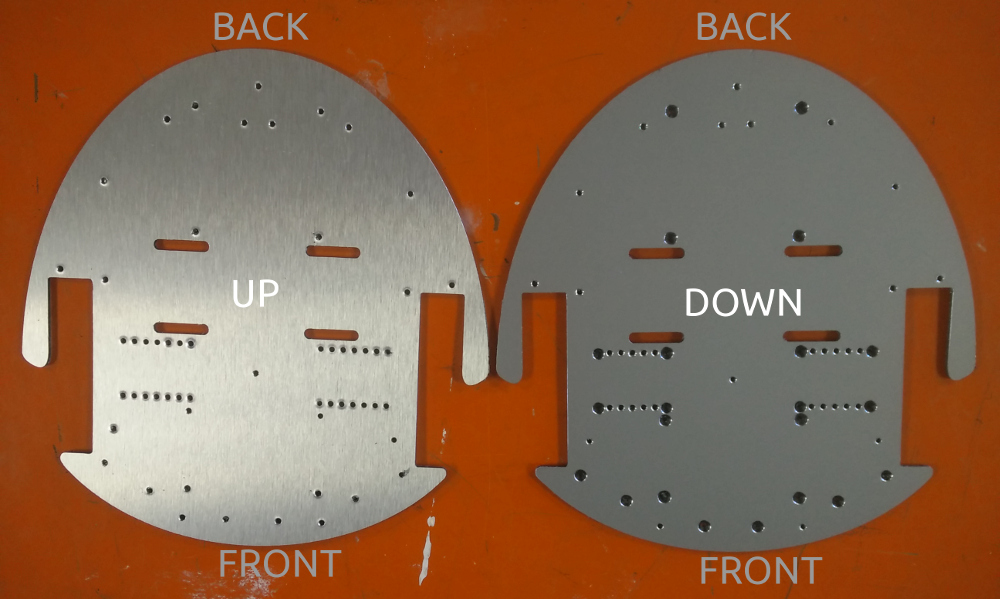
\includegraphics[width=250px]{images/01.jpg}
\caption{The Lower plate.}
\label{fig:01}
\end{figure}

\section{The idler wheel}

First, assembling the idler wheel. Here are the needed parts (Figure \ref{fig:02}):

\begin{figure}[H]
\center
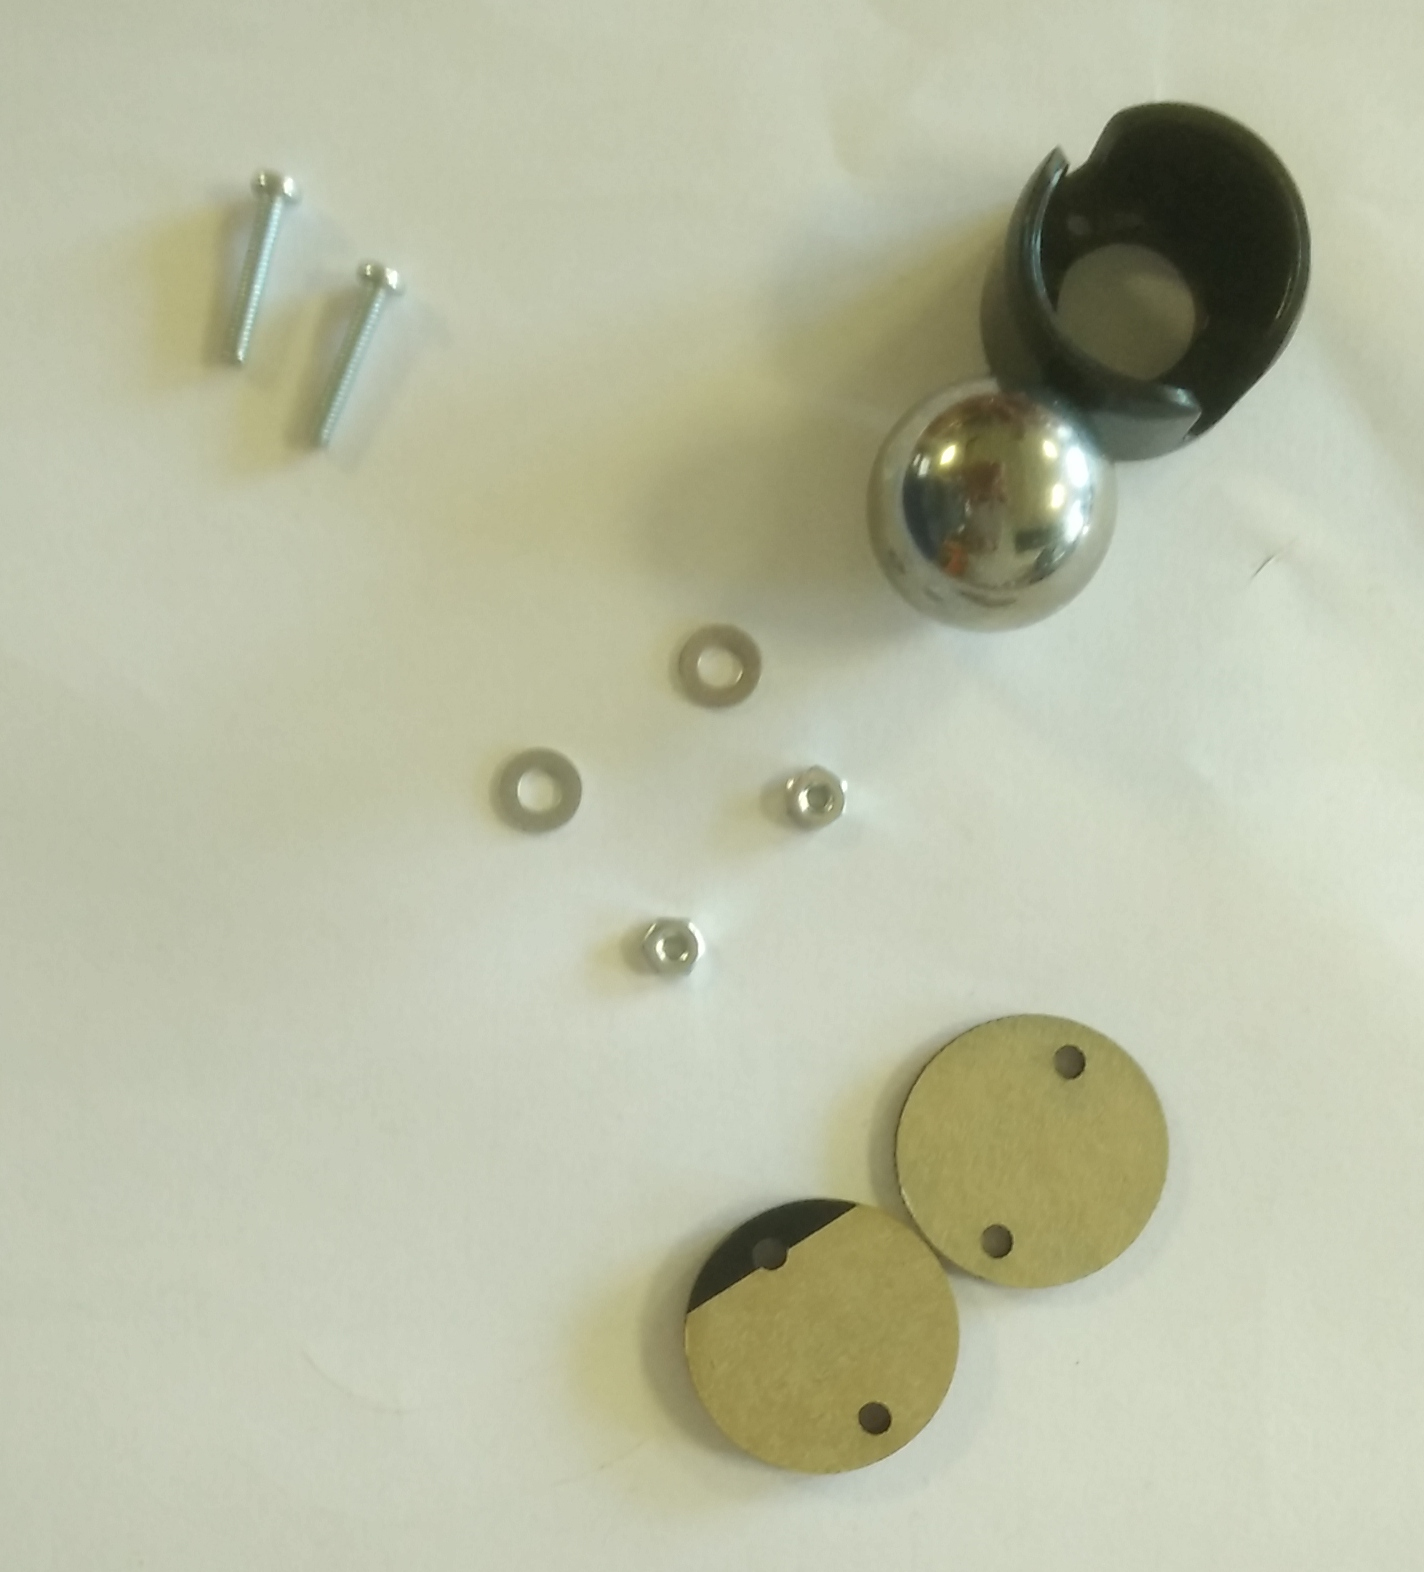
\includegraphics[width=100px]{images/02.jpg}
\caption{The idler wheel components.}
\label{fig:02}
\end{figure}

Screw the support to the low plate, as depicted in Figure \ref{fig:03}.

\begin{figure}[H]
\center
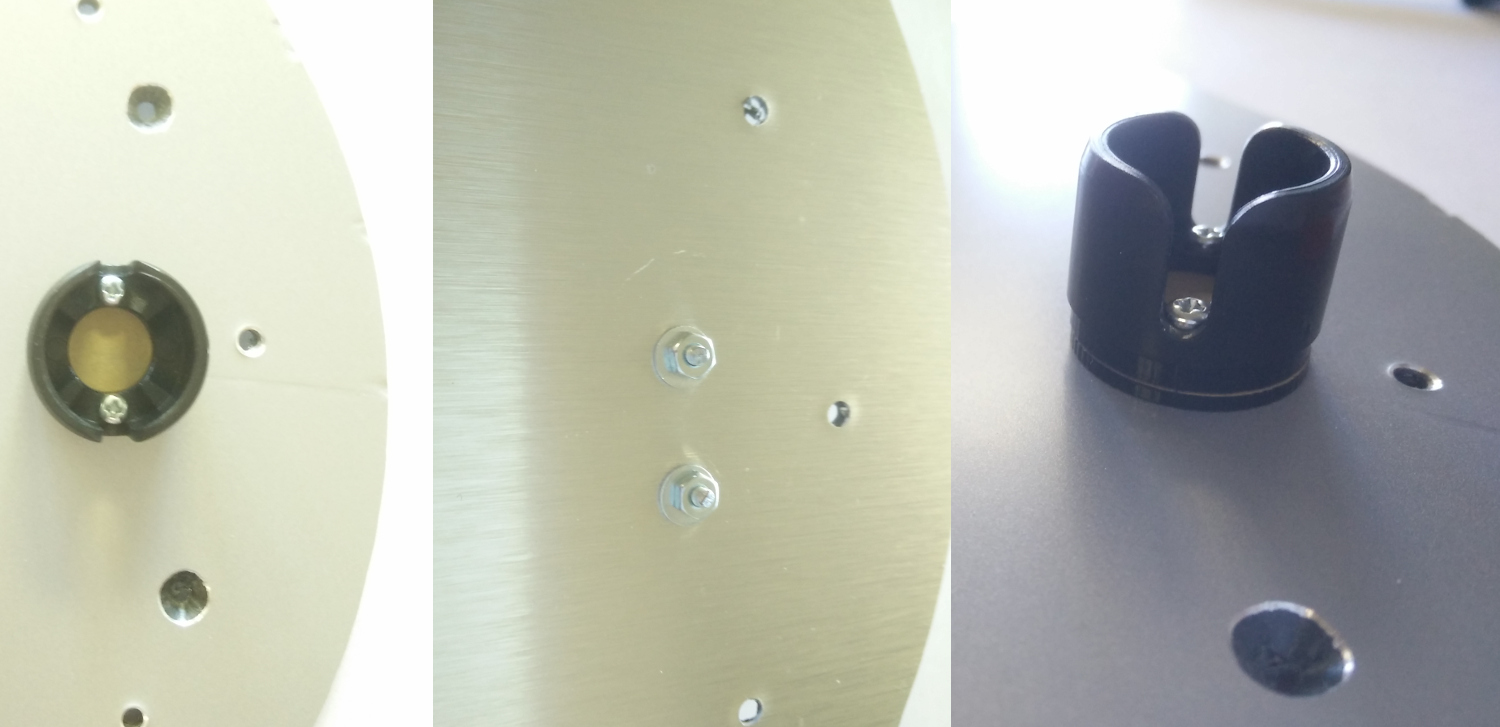
\includegraphics[width=250px]{images/03.jpg}
\caption{The idler wheel components.}
\label{fig:03}
\end{figure}

Be carefull with the support facing \textbf{down}. You sould have the result depicted in Figure \ref{fig:04}.

\begin{figure}[H]
\center
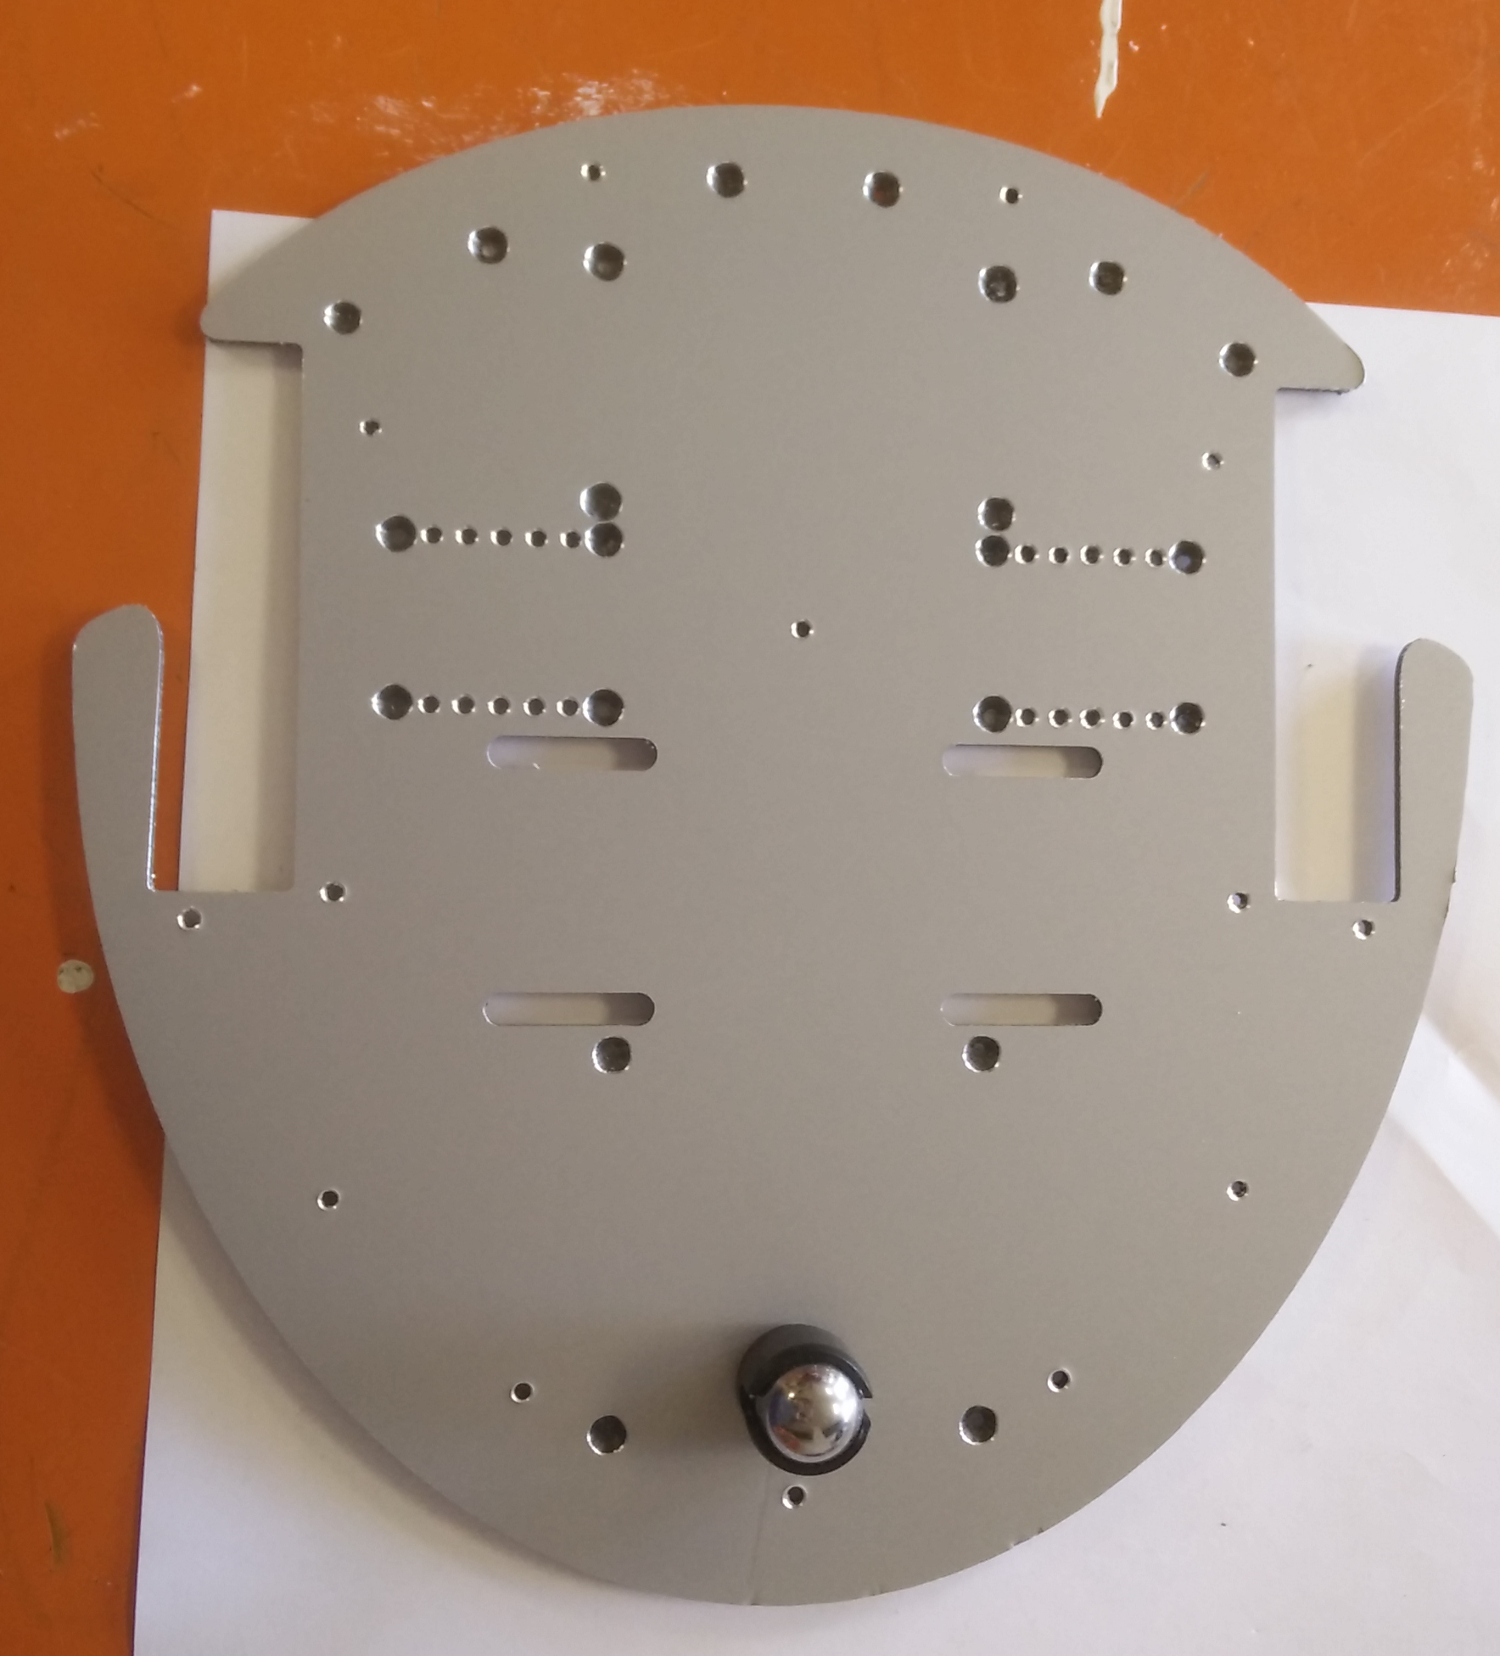
\includegraphics[width=150px]{images/04.jpg}
\caption{The idler fixed to the first plate.}
\label{fig:04}
\end{figure}

\section{The motor supports}

Then assemble the motor supports (to fixe the motors later). Figure \ref{fig:05} presents the needed components.

\begin{figure}[H]
\center
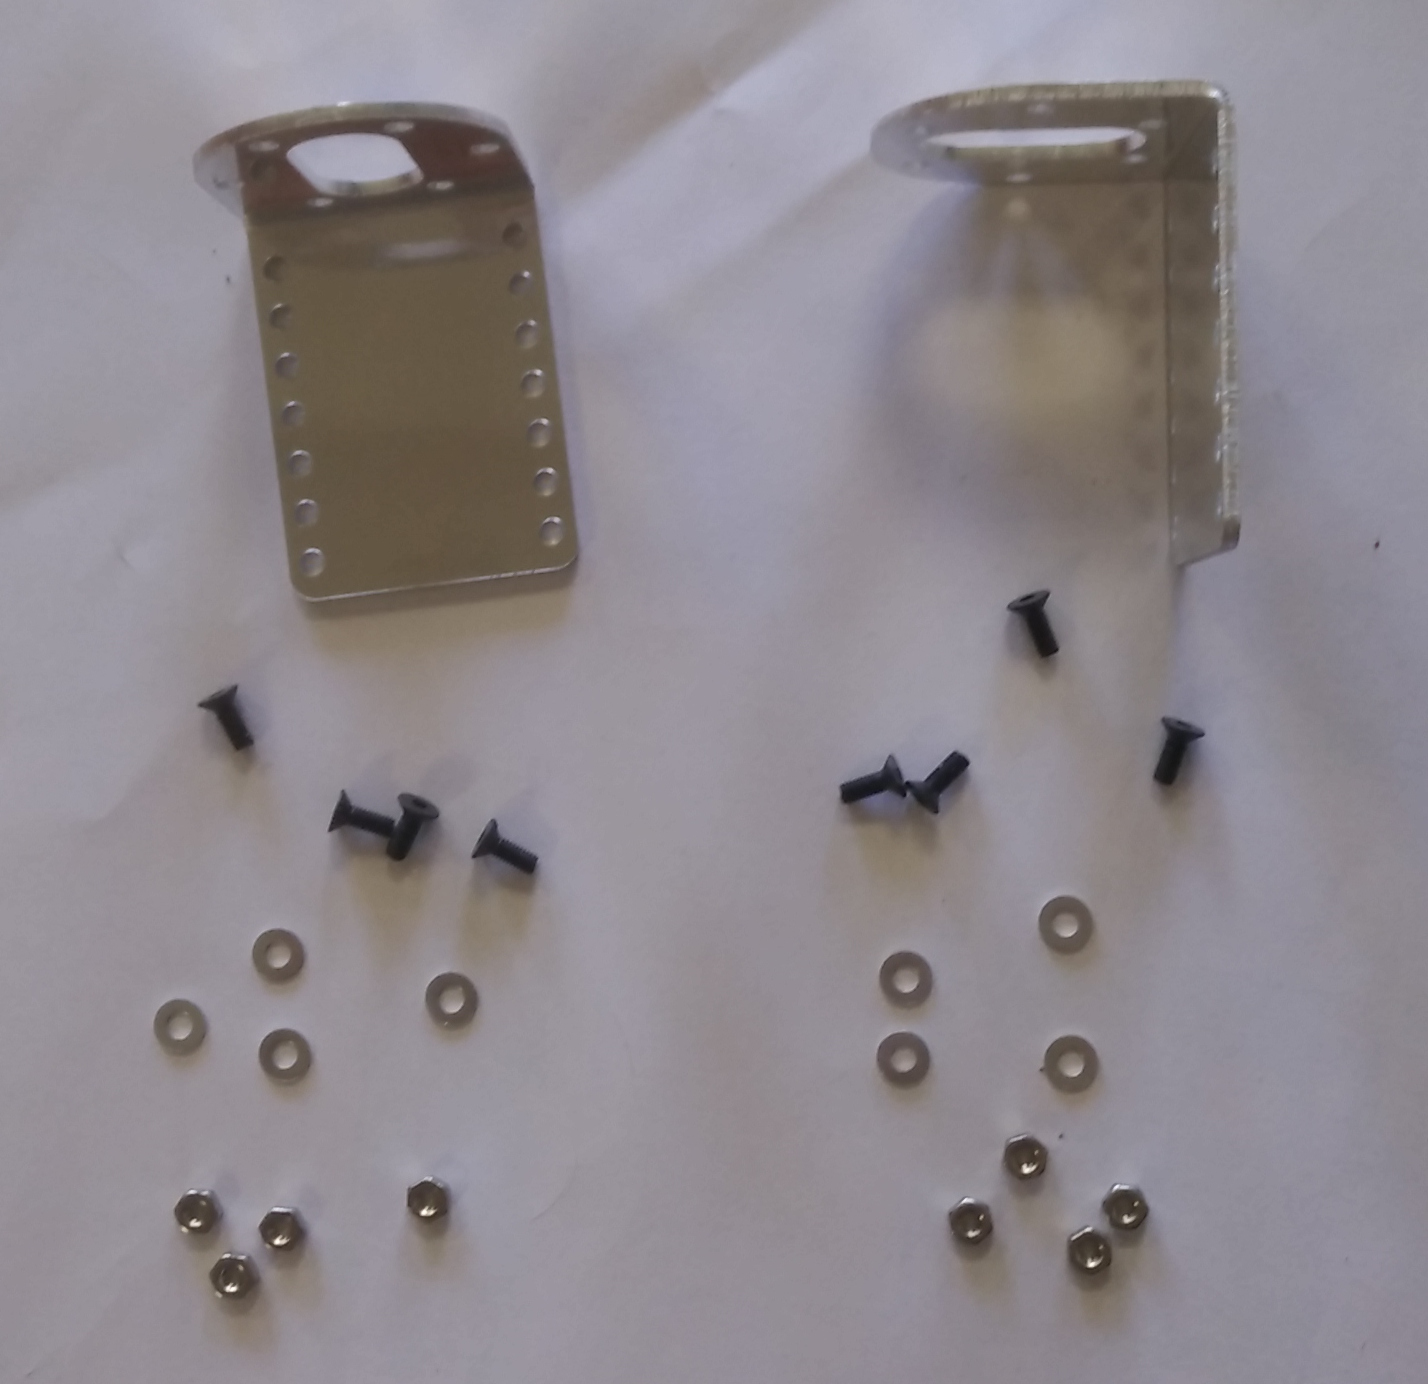
\includegraphics[width=150px]{images/05.jpg}
\caption{The motor support components.}
\label{fig:05}
\end{figure}

The supports need to be assembled as depicted in Figure \ref{fig:06} and \ref{fig:07}. Once again, be carrefull that the support are facing \textbf{up}.

\begin{figure}[H]
\center
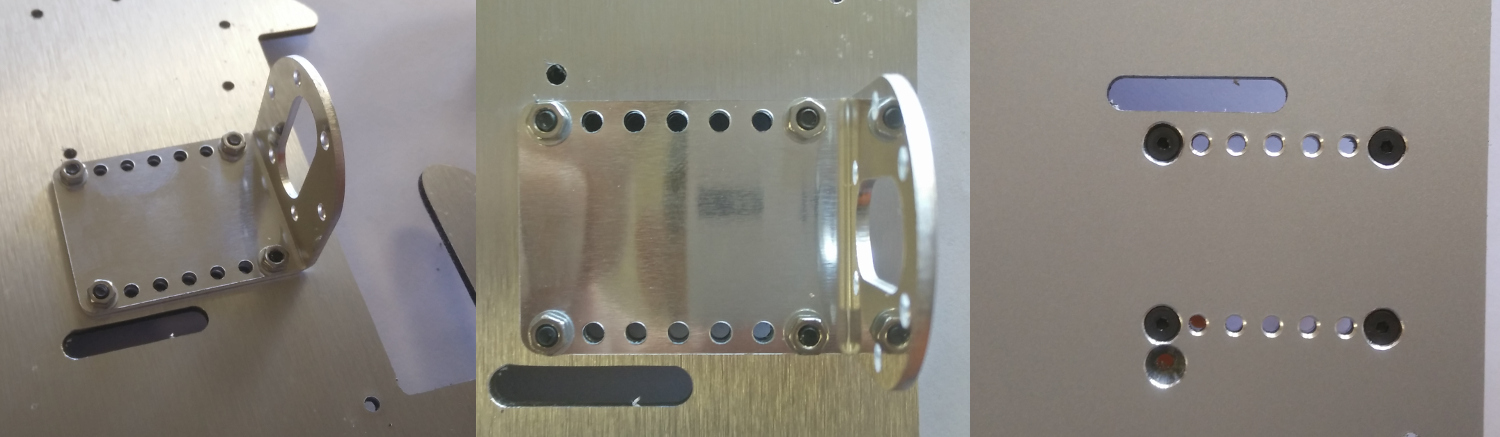
\includegraphics[width=300px]{images/06.jpg}
\caption{One fixed motor support.}
\label{fig:06}
\end{figure}

\begin{figure}[H]
\center
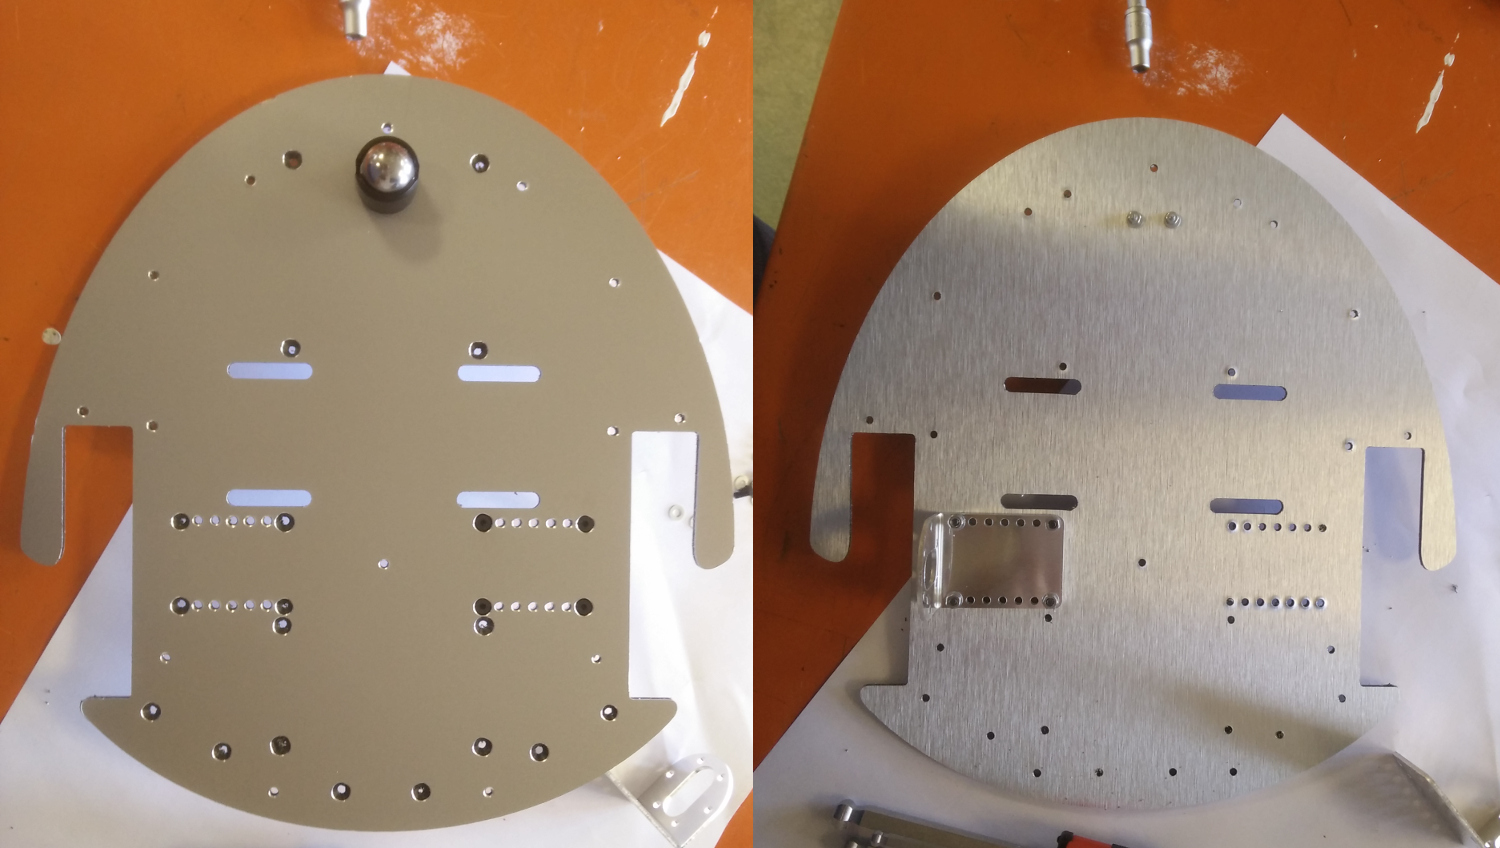
\includegraphics[width=300px]{images/07.jpg}
\caption{One fixed motor support (larger view).}
\label{fig:07}
\end{figure}

Once one support is fixed, assemble the second one to obtain the results depicted in Figures \ref{fig:08}.

\begin{figure}[H]
\center
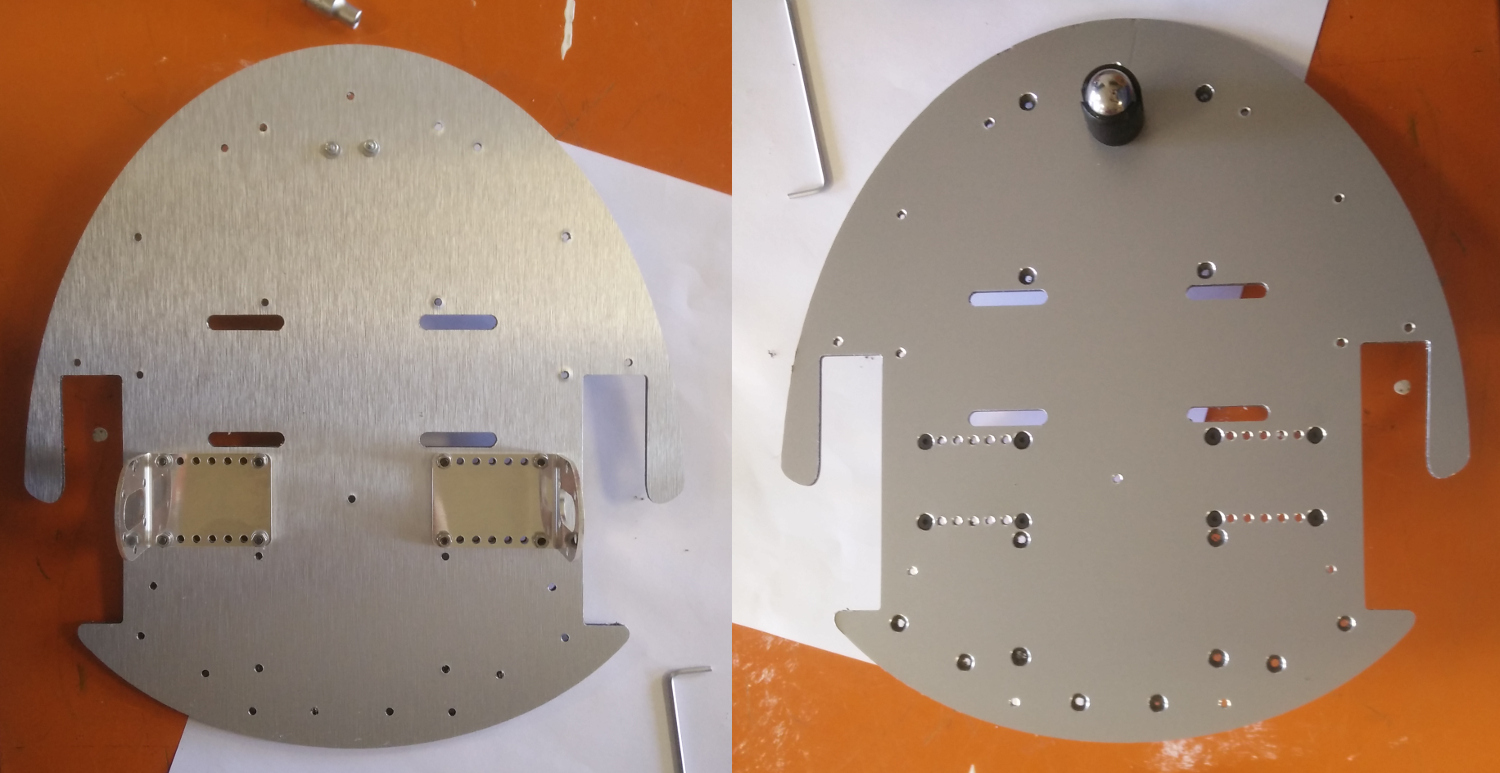
\includegraphics[width=300px]{images/08.jpg}
\caption{Fixed motor supports.}
\label{fig:08}
\end{figure}

\section{The motors}

The motors can now be fixed using the supports. The needed components are depicted in Figure \ref{fig:09}, and the expected results are depicted in Figure \ref{fig:10}. Be carefull to fix the motor well : the rotor close to the plate.

\begin{figure}[H]
\center
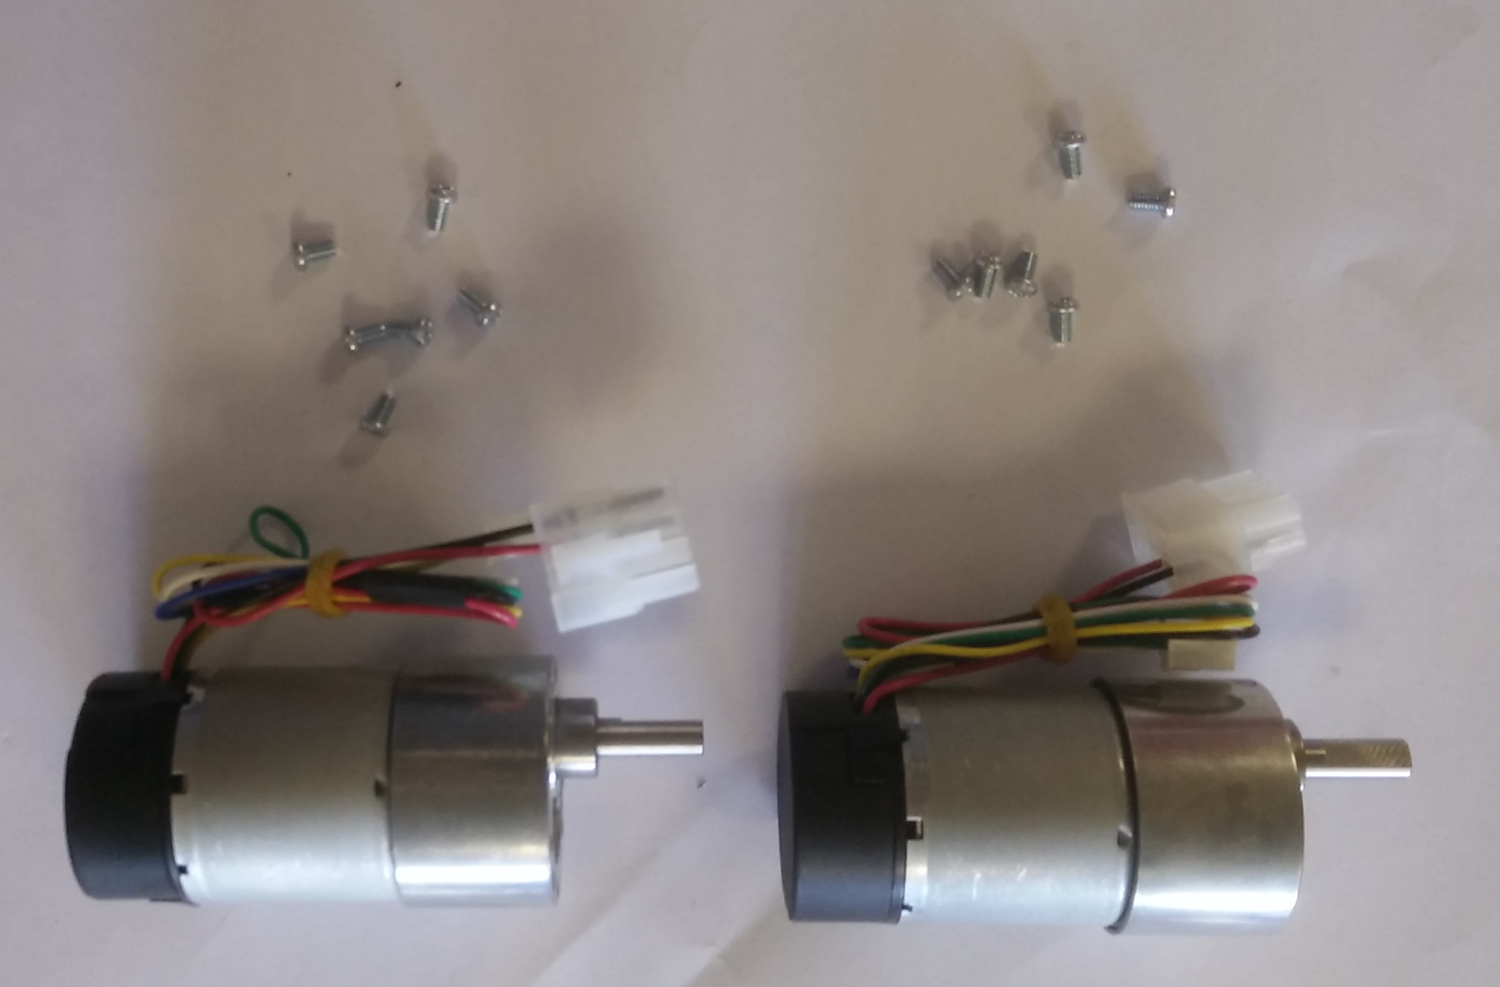
\includegraphics[width=200px]{images/09.jpg}
\caption{The motor components.}
\label{fig:09}
\end{figure}


\begin{figure}[H]
\center
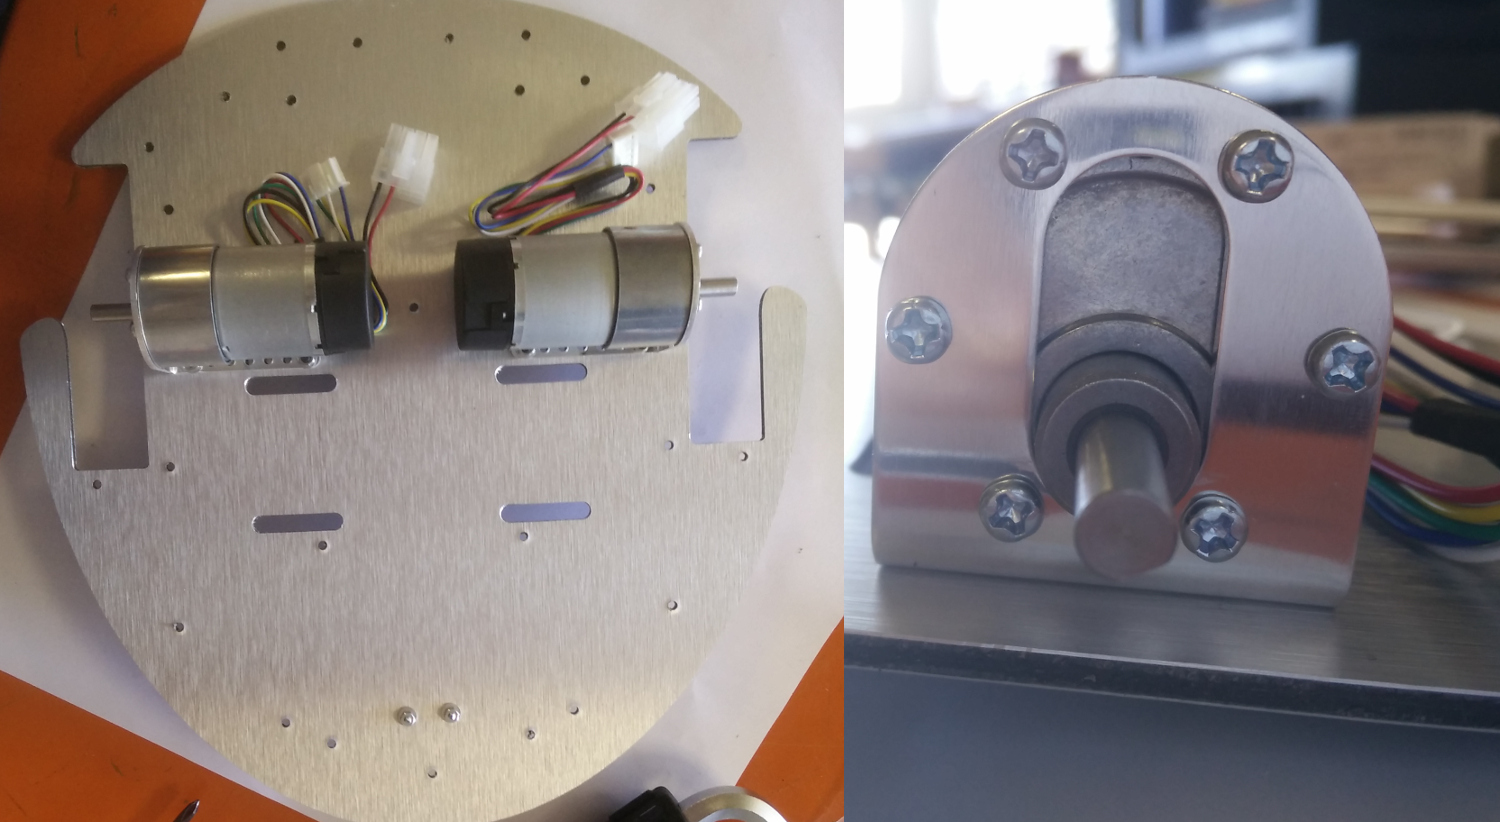
\includegraphics[width=300px]{images/10.jpg}
\caption{Fixed motors.}
\label{fig:10}
\end{figure}

\section{The wheels}

Before fixing the wheels to the motors, it is needed to fix the wheel supports to the wheels. The needed components for this step are depicted in Figure \ref{fig:11} and the expected results are depicted in Figure \ref{fig:12}.

\begin{figure}[H]
\center
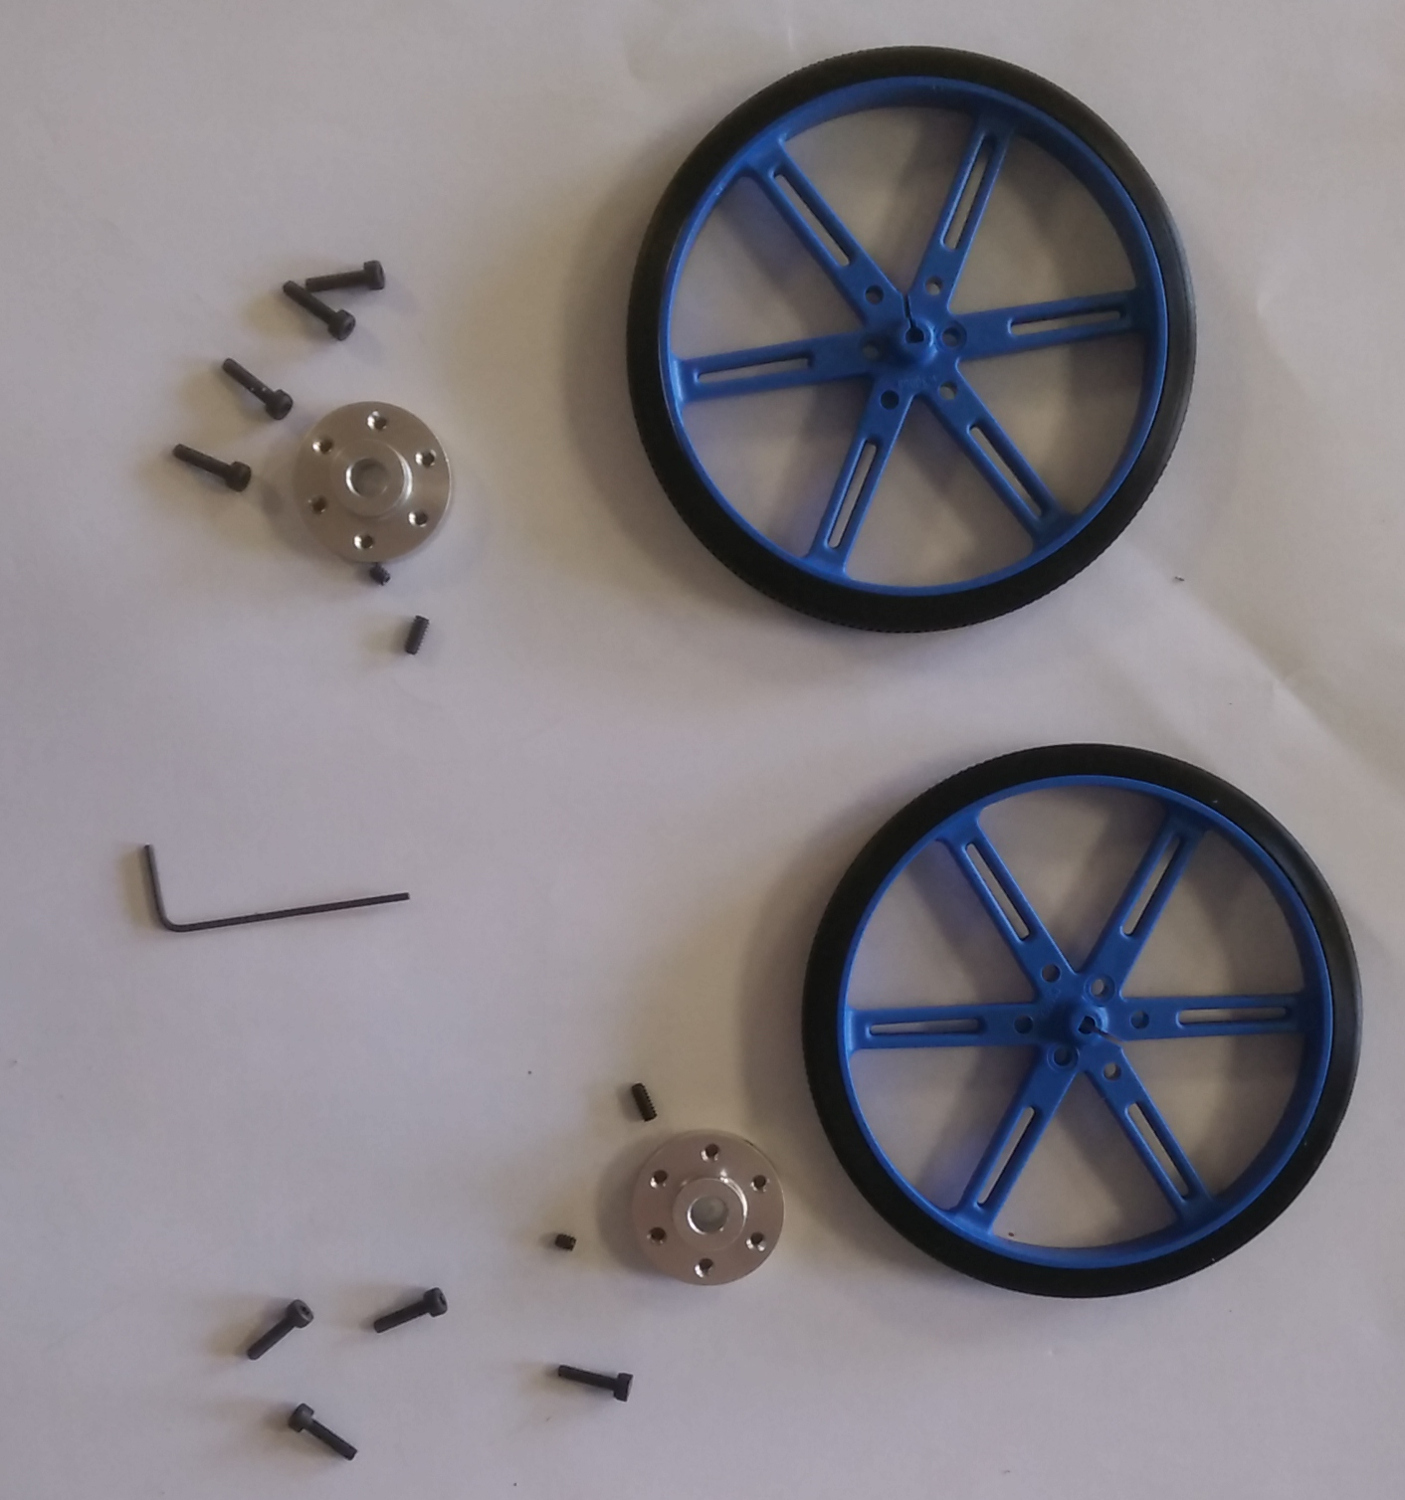
\includegraphics[width=150px]{images/11.jpg}
\caption{The wheel support components.}
\label{fig:11}
\end{figure}


\begin{figure}[H]
\center
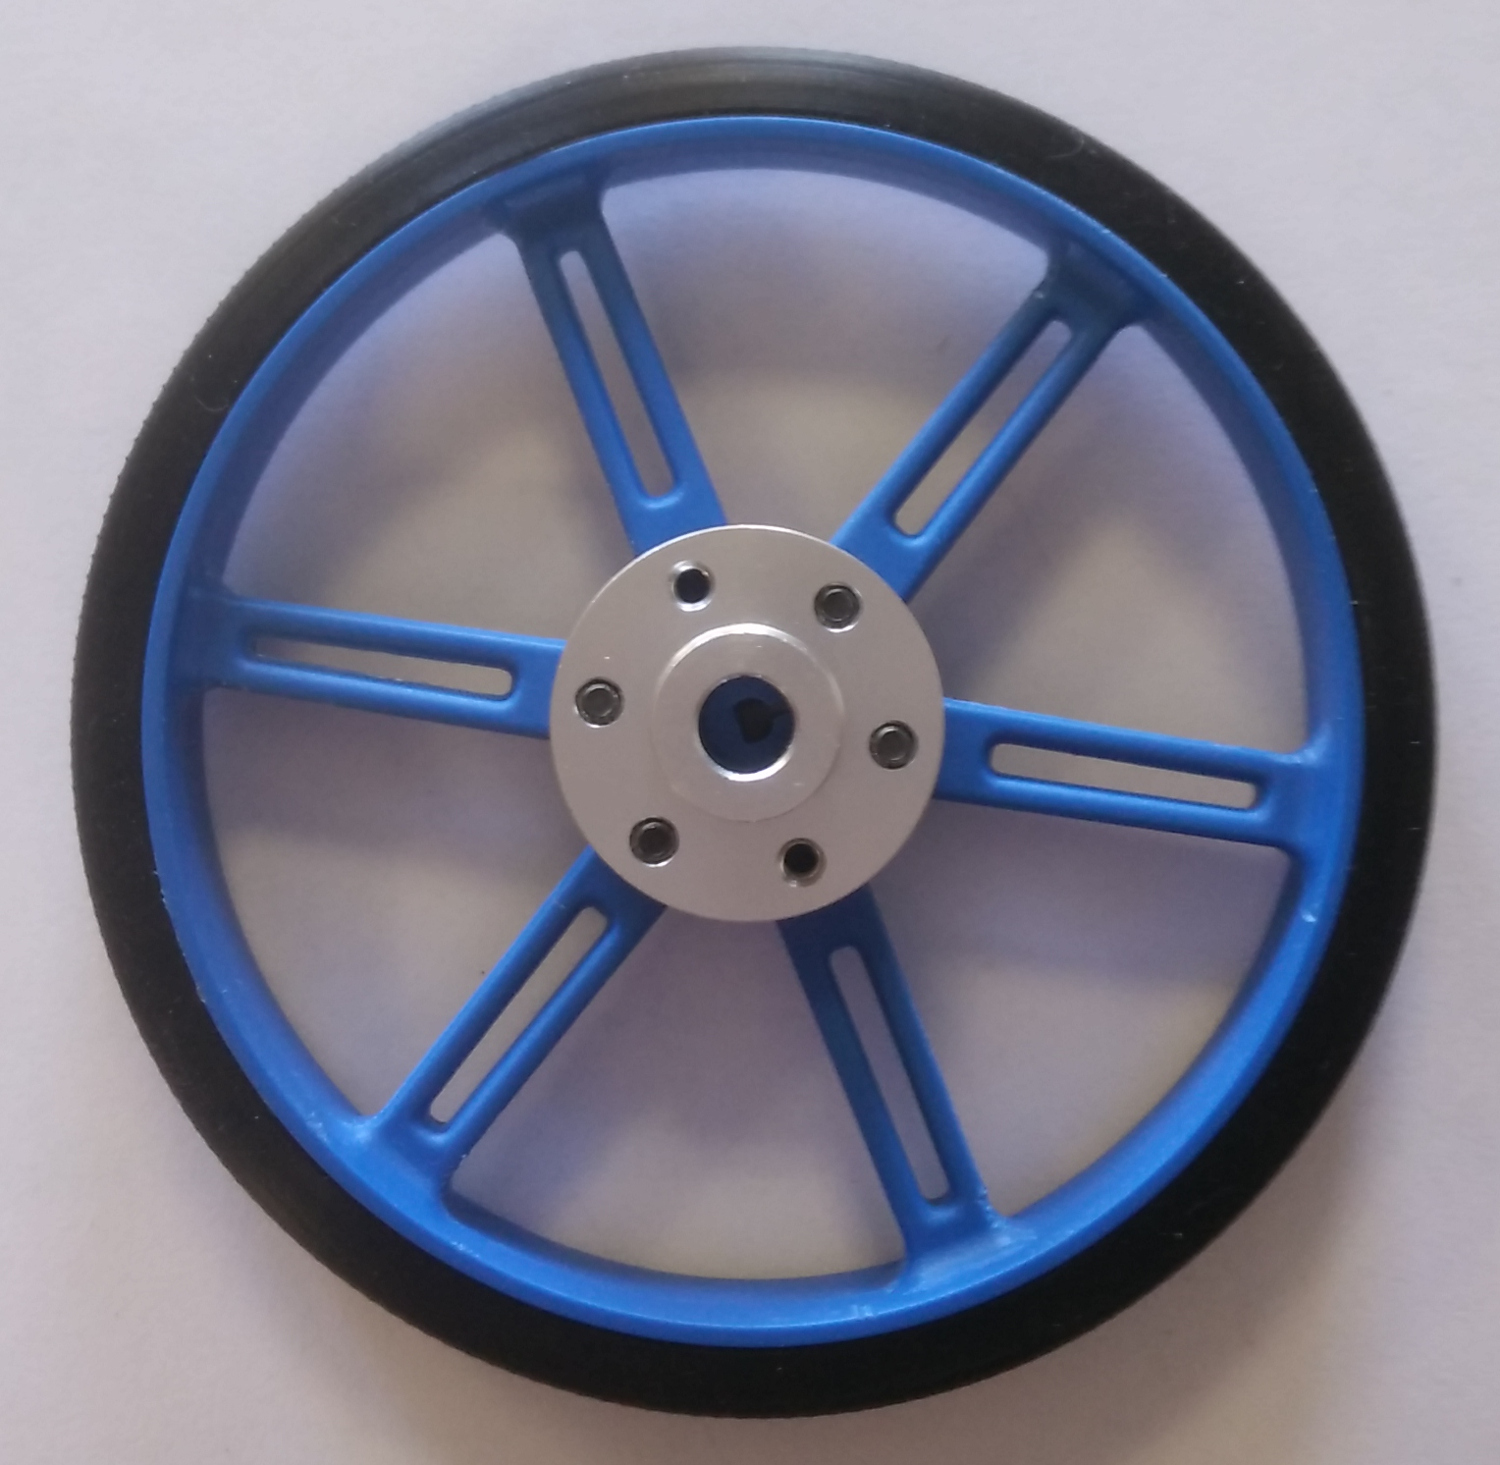
\includegraphics[width=150px]{images/12.jpg}
\caption{Fixed wheel supports.}
\label{fig:12}
\end{figure}

Once the wheel supports are fixed, the wheels can be fix to the motors. The needed components for this step are depicted in Figure \ref{fig:13} while the results are depicted in Figure \ref{fig:14}.

\begin{figure}[H]
\center
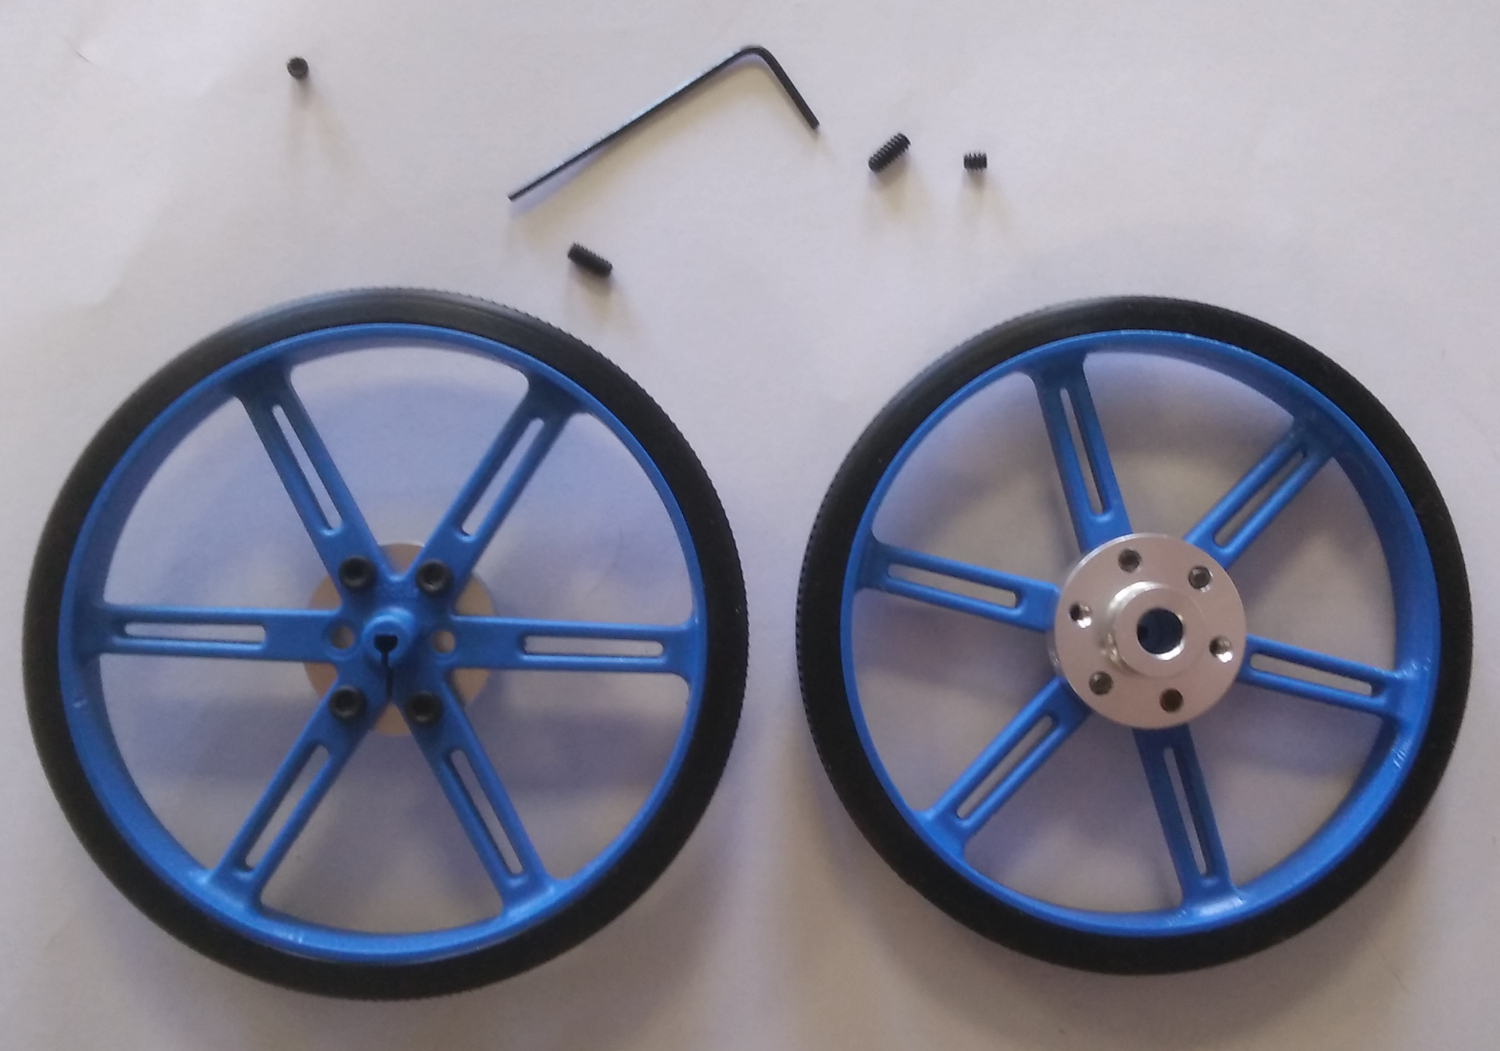
\includegraphics[width=200px]{images/13.jpg}
\caption{The components to fix the wheels to the motors.}
\label{fig:13}
\end{figure}


\begin{figure}[H]
\center
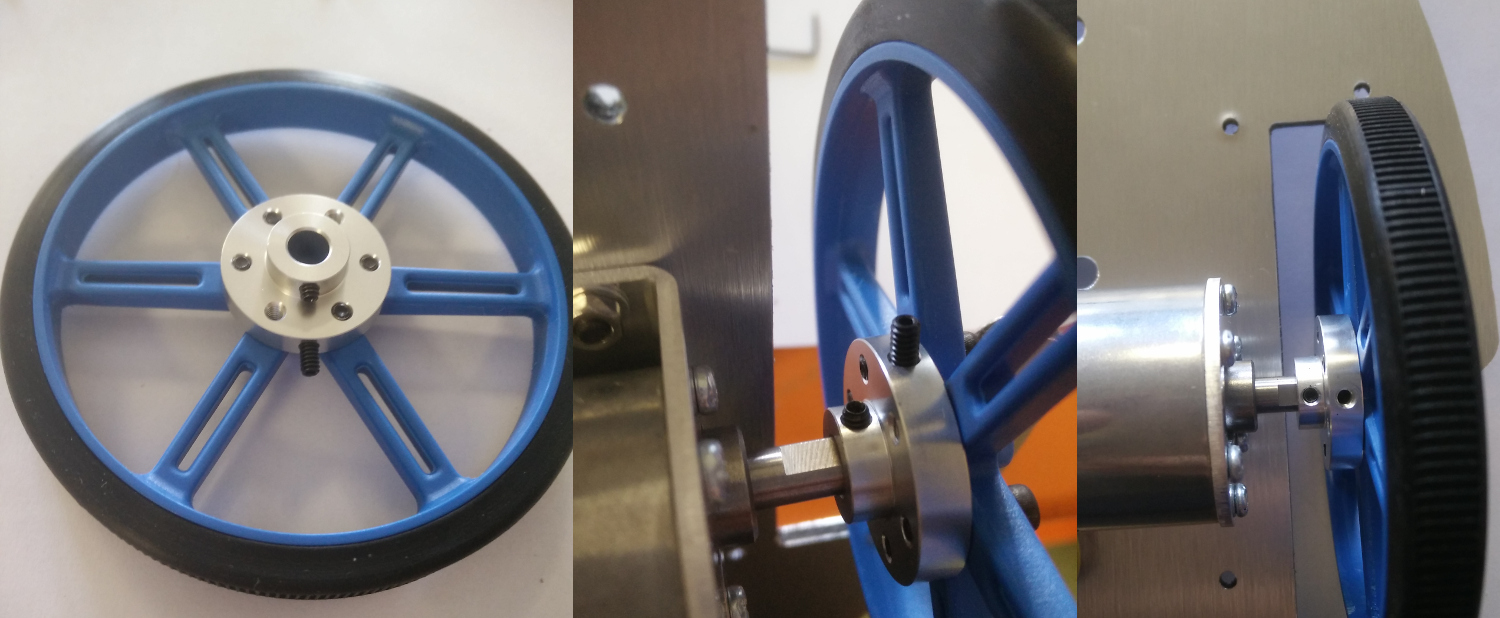
\includegraphics[width=300px]{images/14.jpg}
\caption{Fixed wheels.}
\label{fig:14}
\end{figure}

A this step you should have the result depicted in Figure \ref{fig:15}.

\begin{figure}[H]
\center
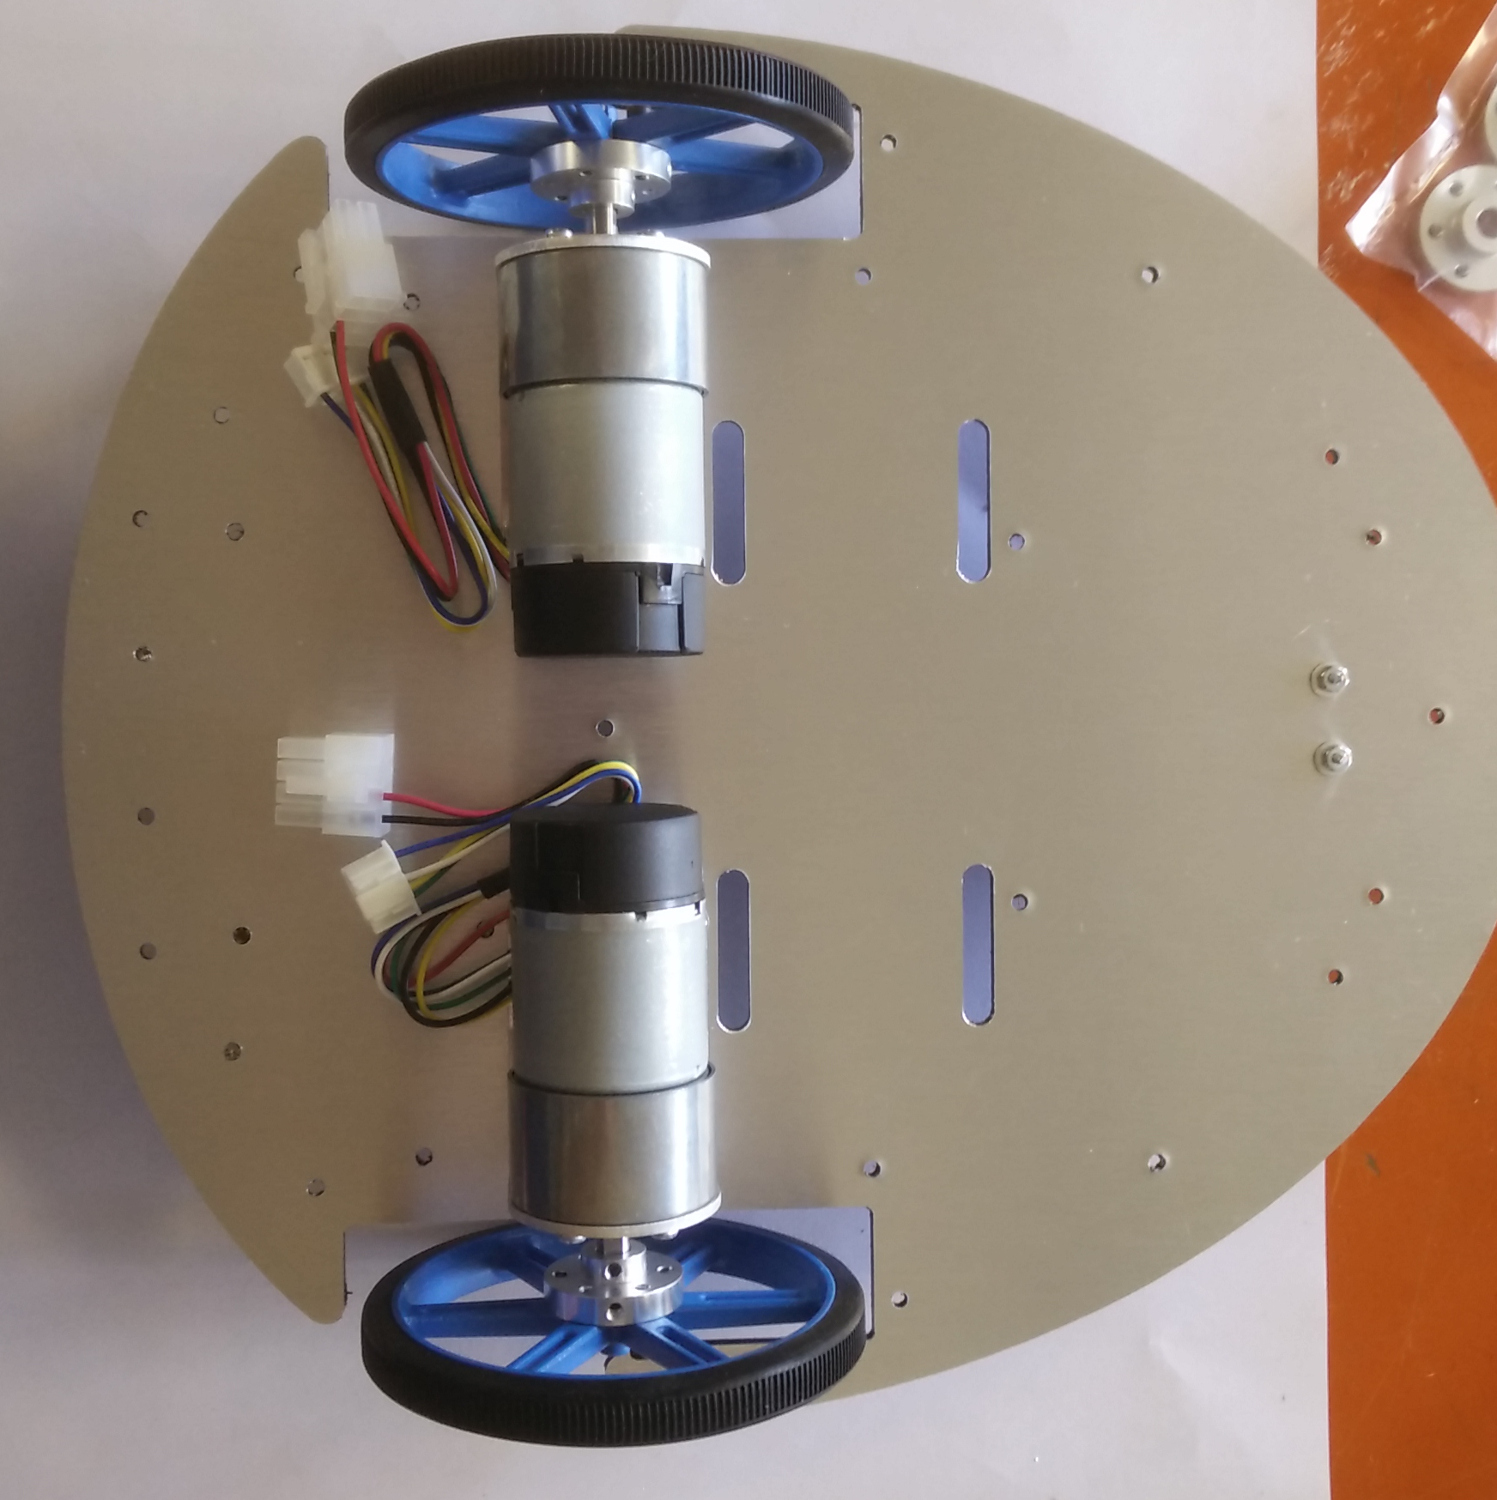
\includegraphics[width=150px]{images/15.jpg}
\caption{Fixed wheels, larger view.}
\label{fig:15}
\end{figure}

\section{Motor boards and power board spacers}

In order to fix the motor boards (to control the motors) and the power board, it is needed to put spacers first. Figure \ref{fig:16} details the needed components for this step and Figure \ref{fig:17} illustrates the expected results.

\begin{figure}[H]
\center
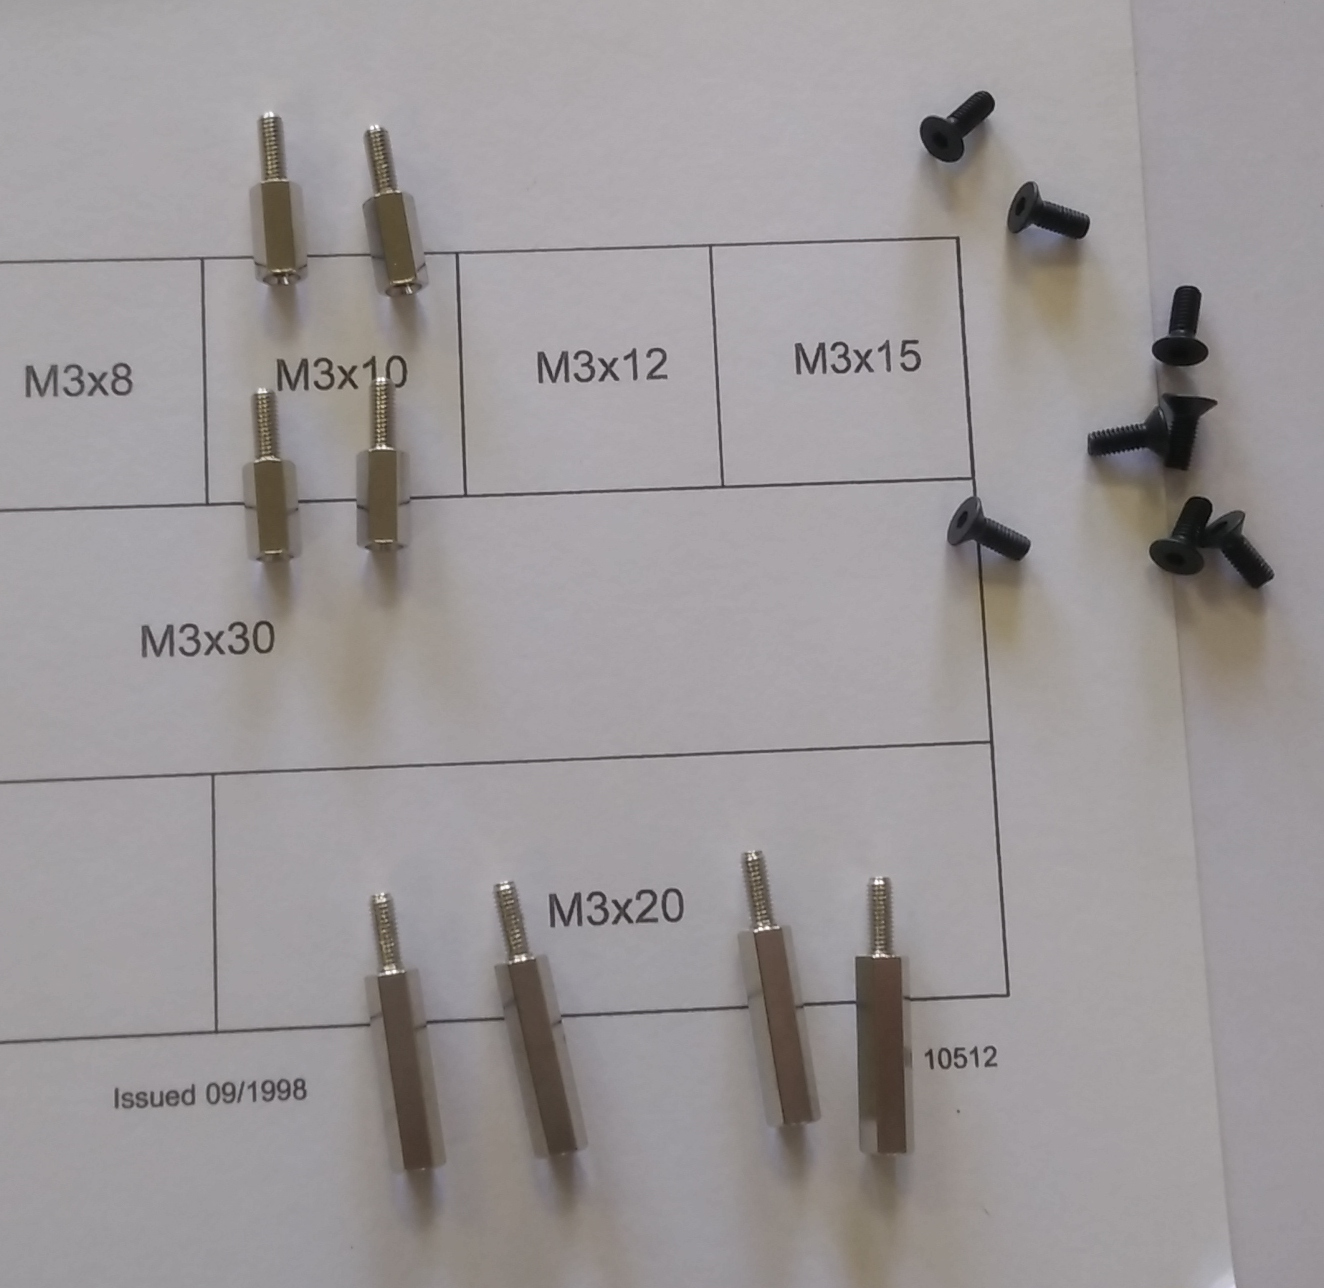
\includegraphics[width=150px]{images/16.jpg}
\caption{Motor board and power board spacers.}
\label{fig:16}
\end{figure}

\begin{figure}[H]
\center
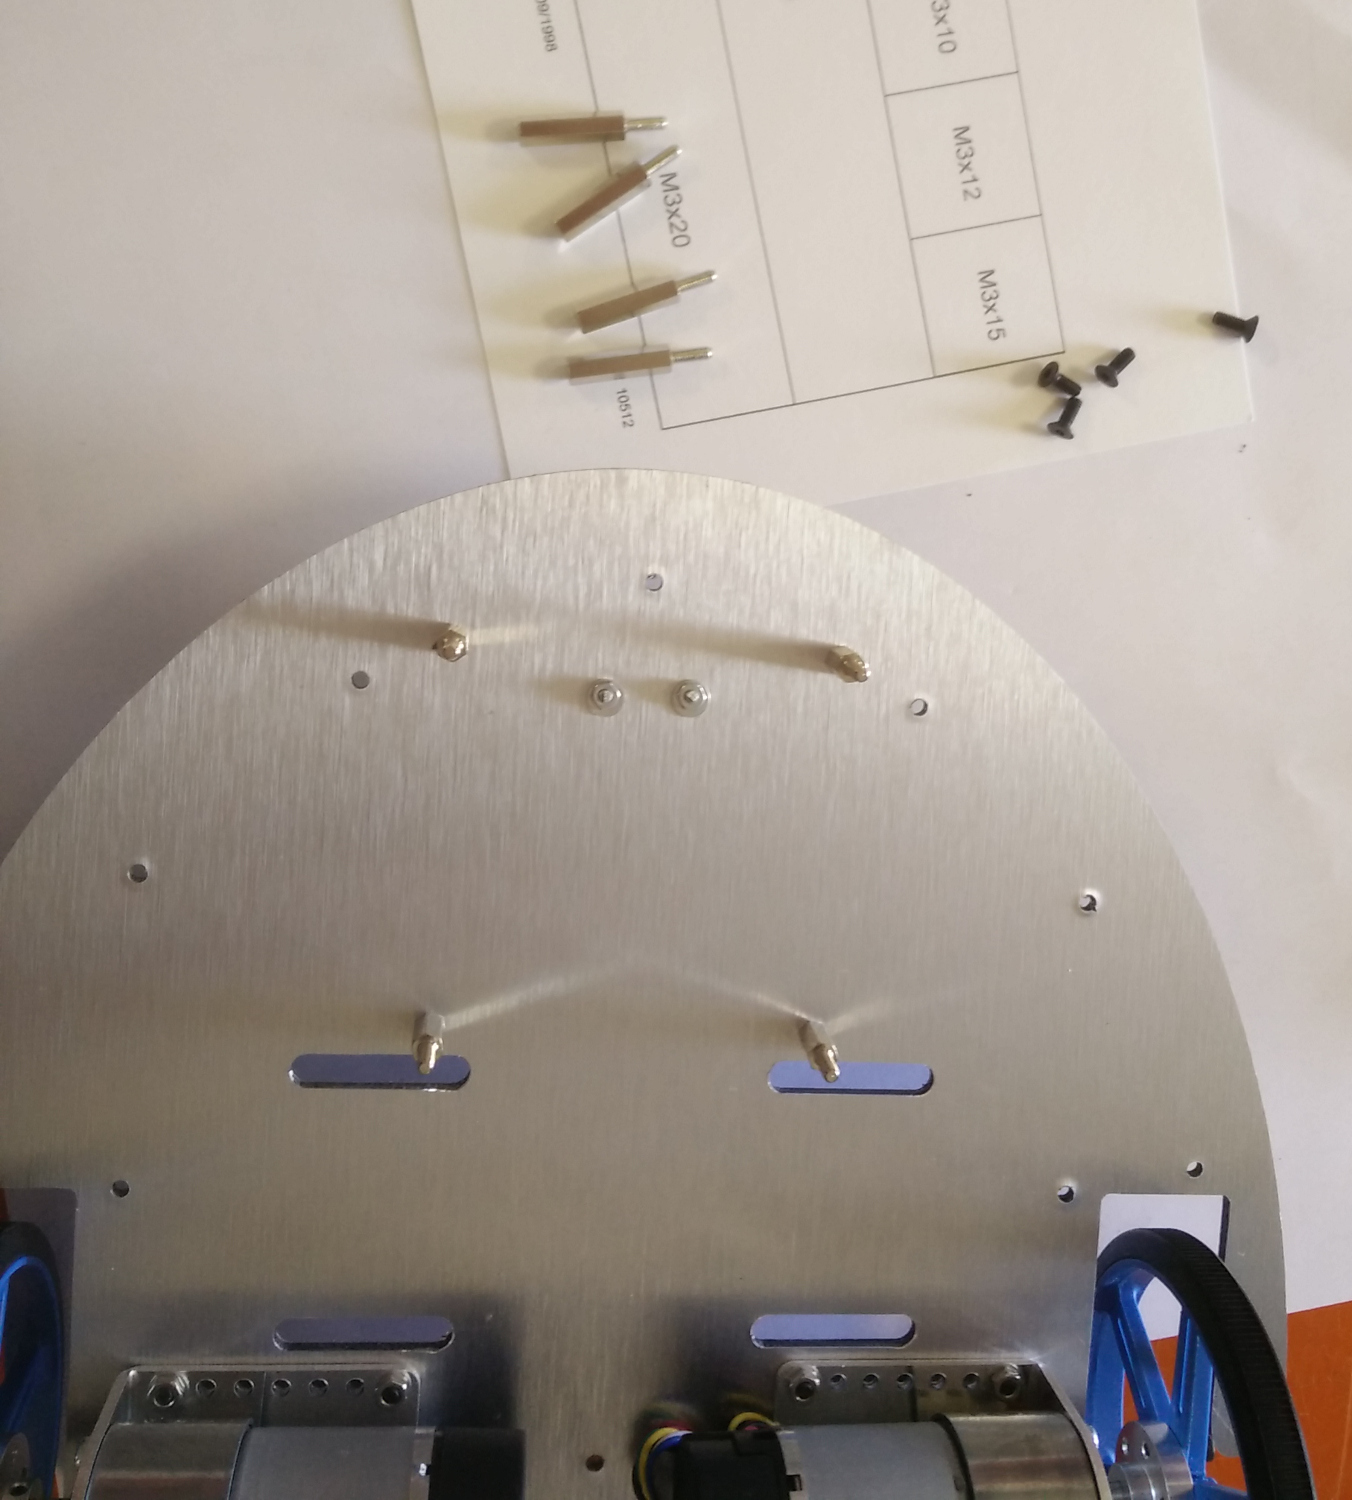
\includegraphics[width=150px]{images/17.jpg}
\caption{Putting the spacers for the motor boards.}
\label{fig:17}
\end{figure}

\begin{figure}[H]
\center
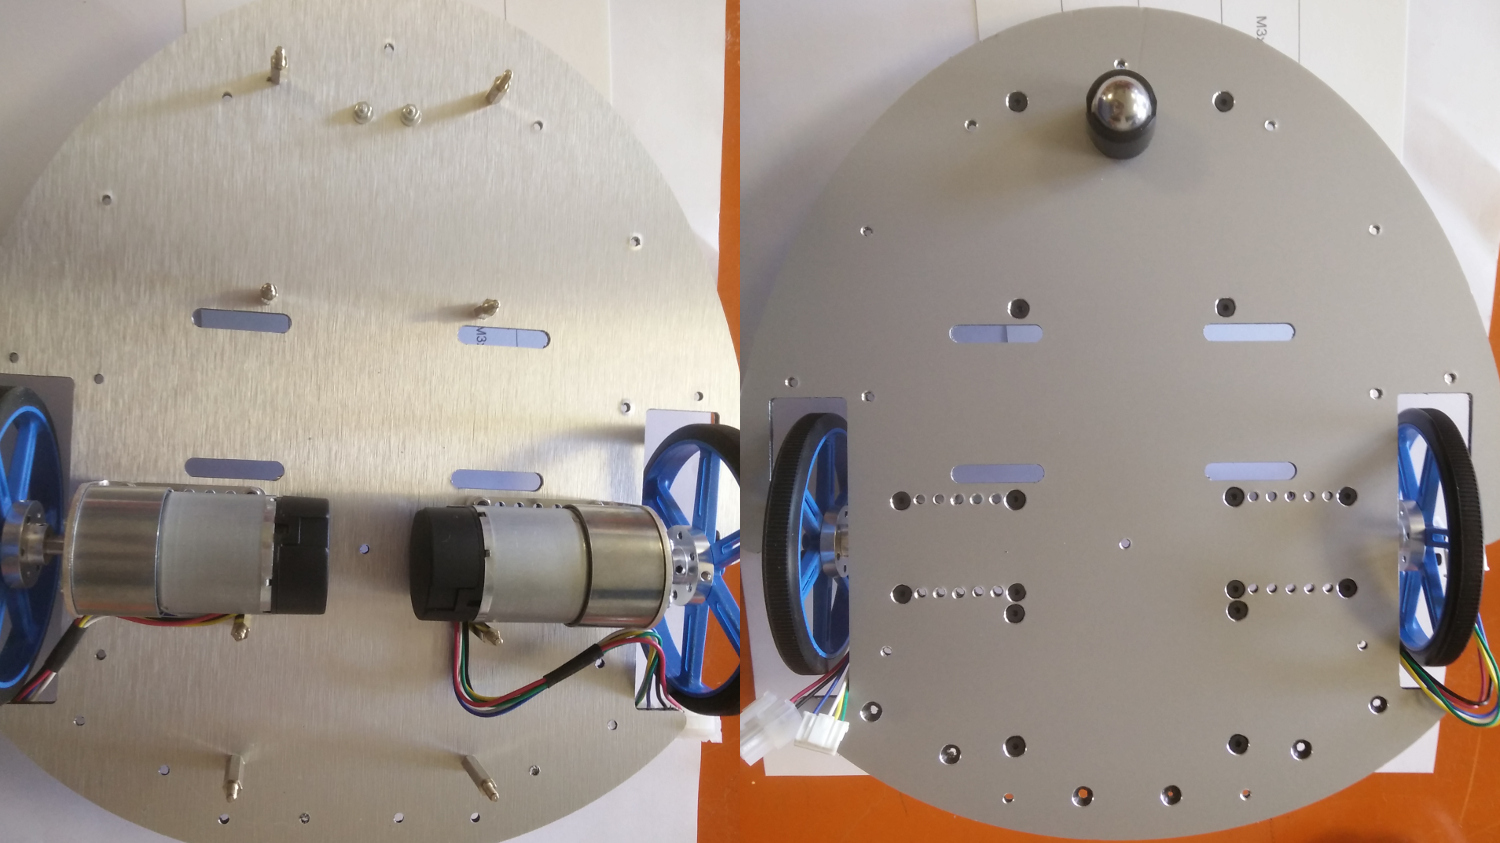
\includegraphics[width=250px]{images/18.jpg}
\caption{Putting the spacers for the power board.}
\label{fig:18}
\end{figure}

\section{Motor boards assembling}

Now it is possible to place the motor boards. The needed components are depicted in Figure \ref{fig:19}. Put the first board as shown in Figure \ref{fig:19}. \textbf{Be carrefull to put the motor wires under the board} as depicted in Figure \ref{fig:20}.

\begin{figure}[H]
\center
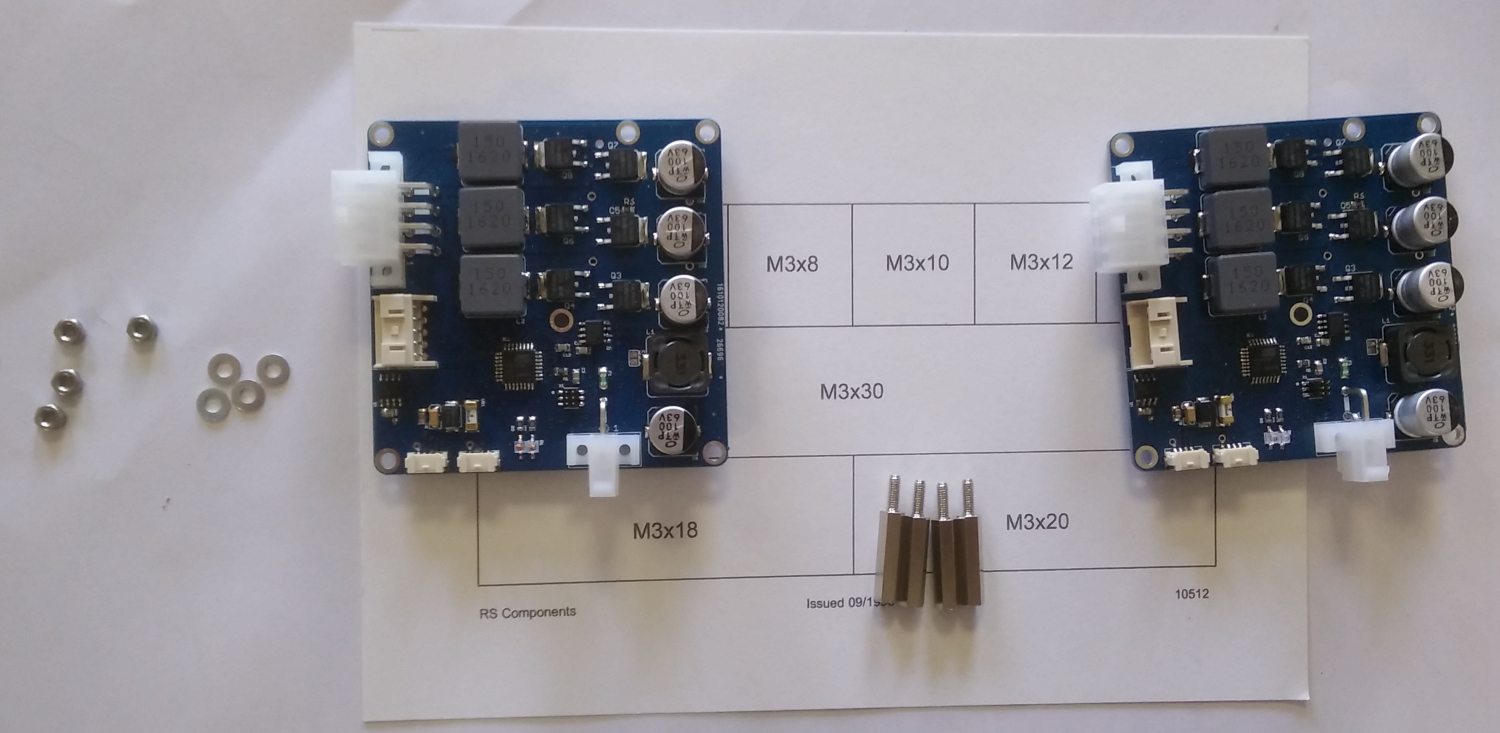
\includegraphics[width=250px]{images/19.jpg}
\caption{The components needed to place the motor boards.}
\label{fig:19}
\end{figure}

\begin{figure}[H]
\center
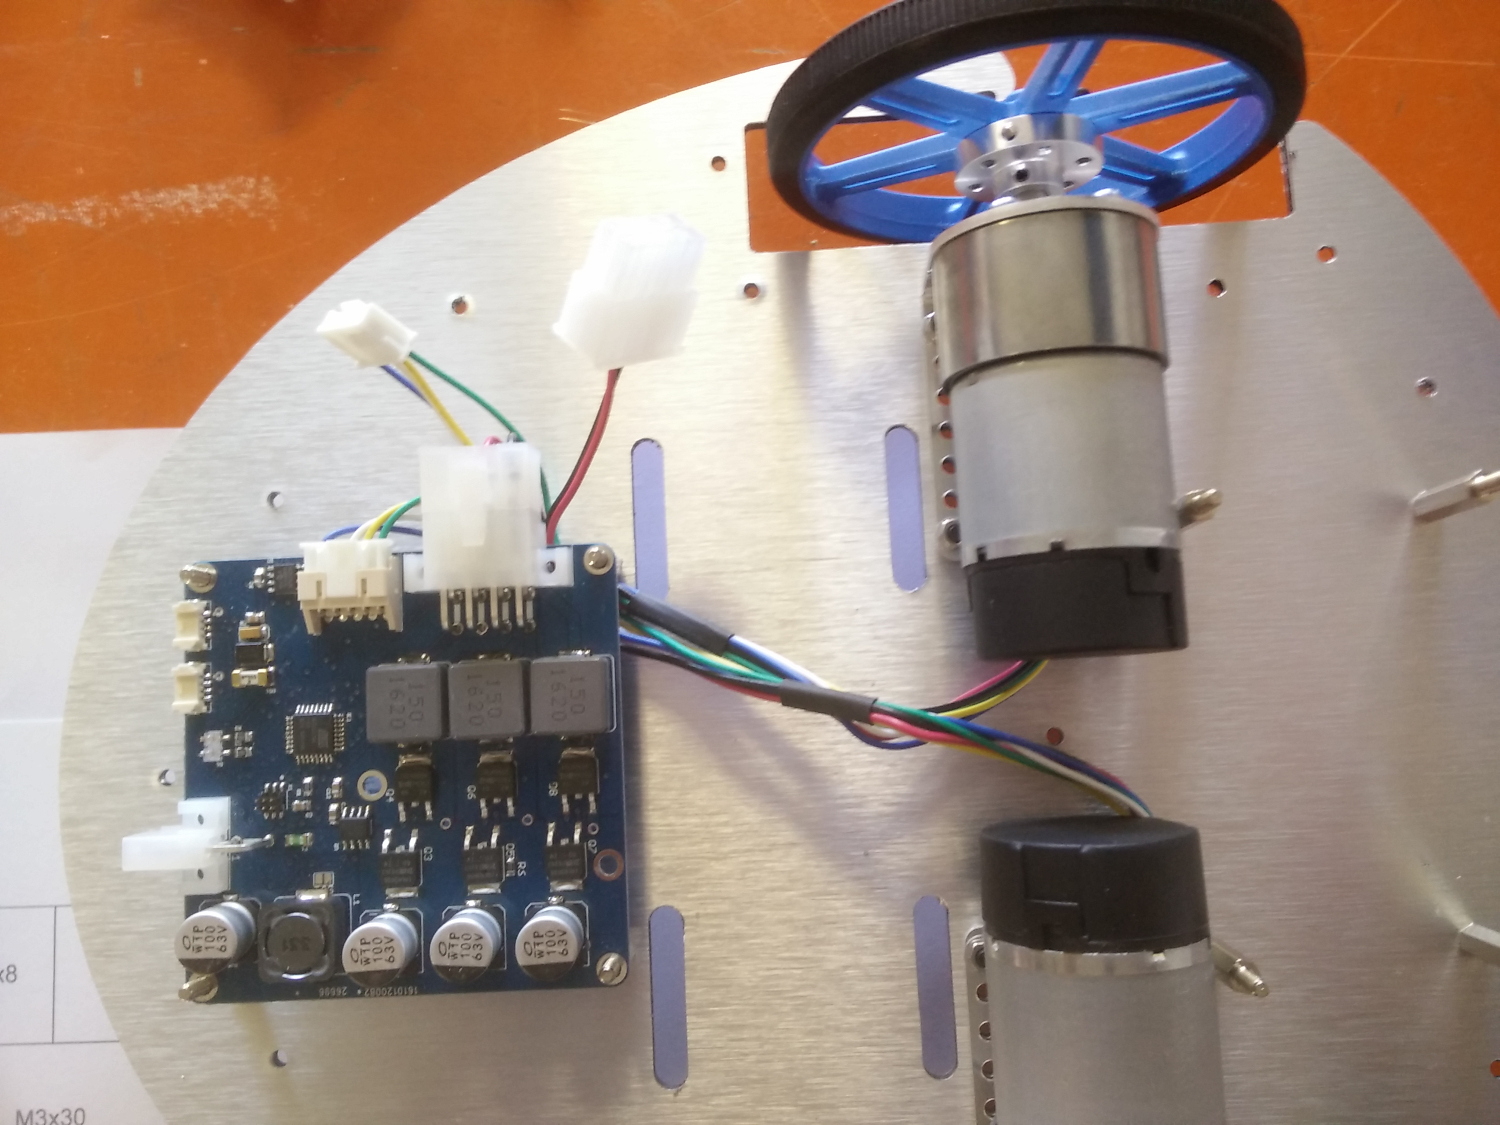
\includegraphics[width=150px]{images/20.jpg}
\caption{The first motor board in place. \textbf{Mind the wires!}}
\label{fig:20}
\end{figure}

Once the first board is in place, put the spacers as shown in Figure \ref{fig:21}.

\begin{figure}[H]
\center
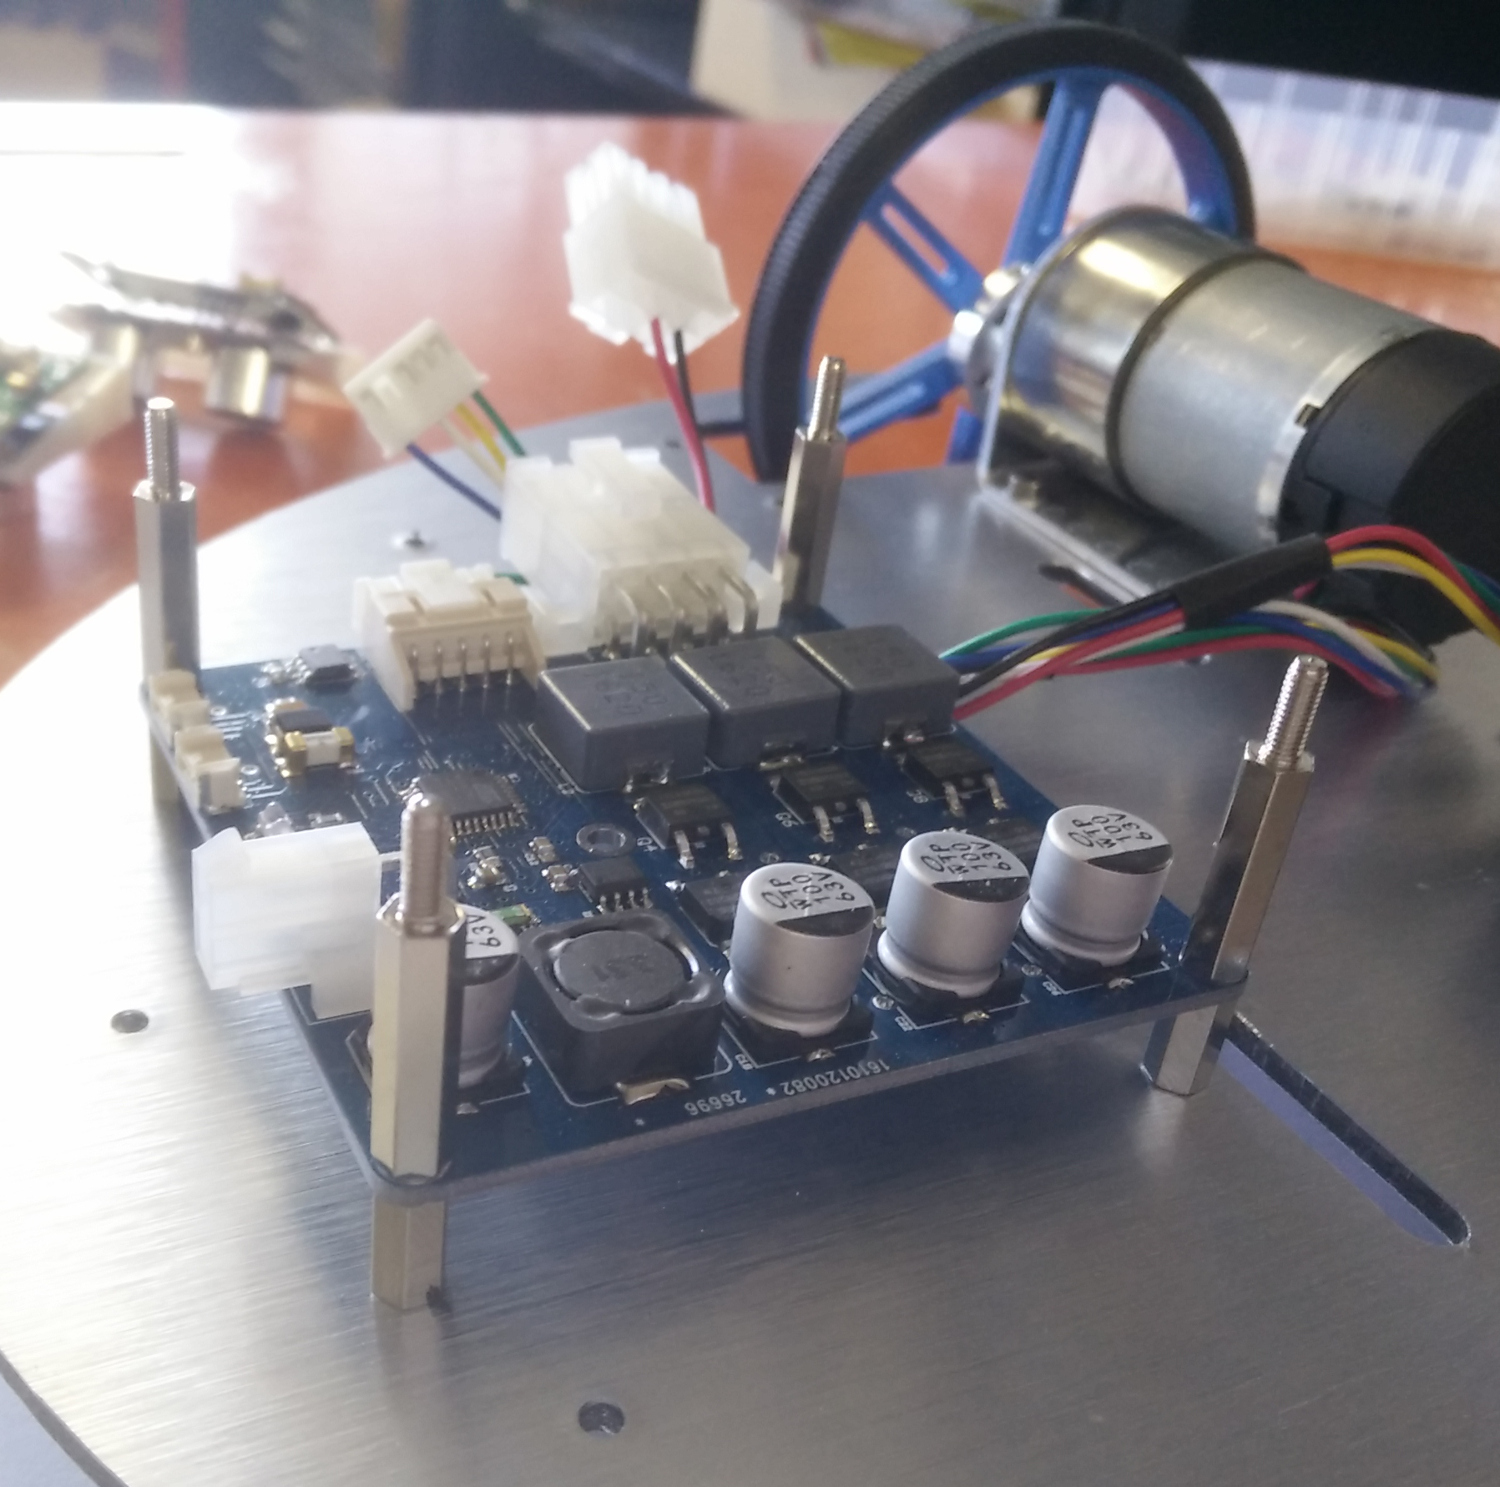
\includegraphics[width=150px]{images/21.jpg}
\caption{The spacers for the second motor board.}
\label{fig:21}
\end{figure}

Then place the second motor board, and wire the motors to the boards, as depicted in Figure \ref{fig:22}.

\begin{figure}[H]
\center
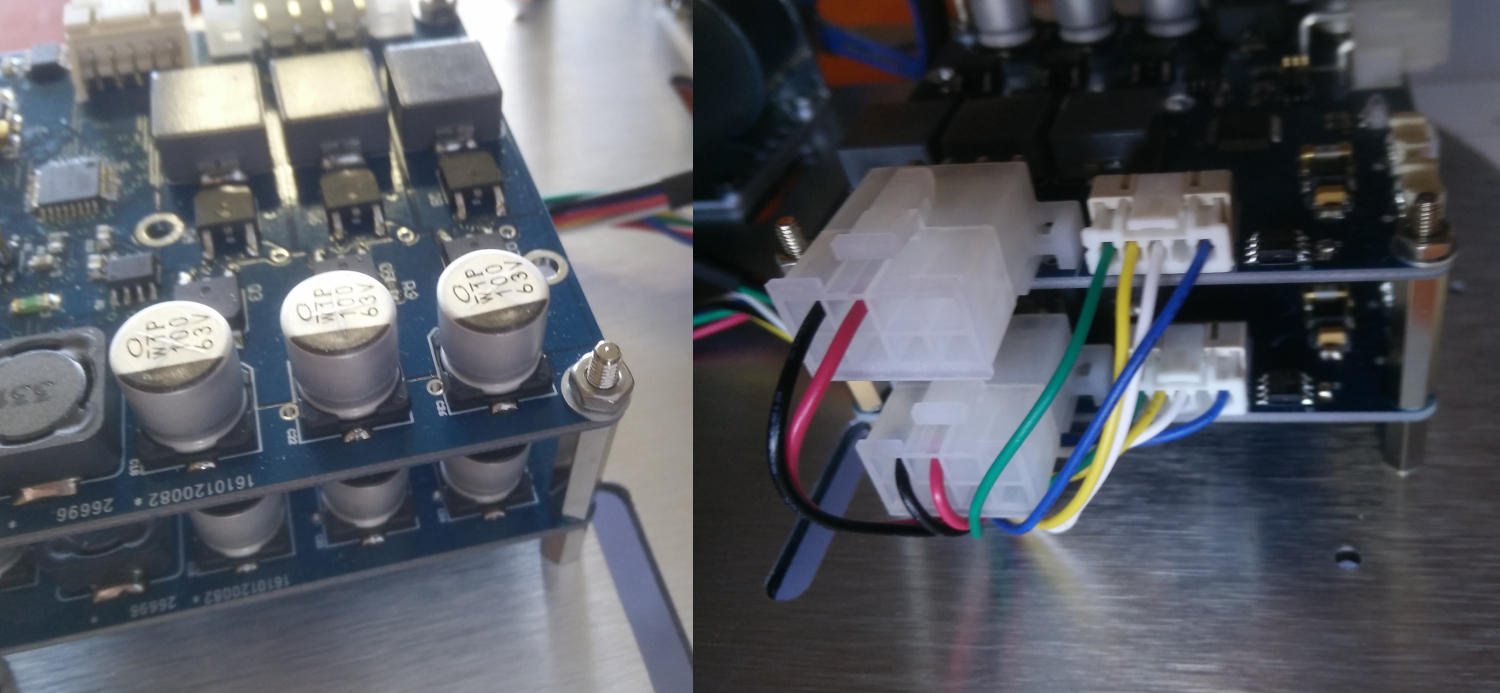
\includegraphics[width=300px]{images/22.jpg}
\caption{Putting the second motor board and wiring the boards.}
\label{fig:22}
\end{figure}

\section{Placing the power board}

The next step is to install the power board on the robot. The needed components are depicted in Figure \ref{fig:23} and the expected result is detailed in Figure \ref{fig:24}. \textbf{Be carefull with the board orientation}.

\begin{figure}[H]
\center
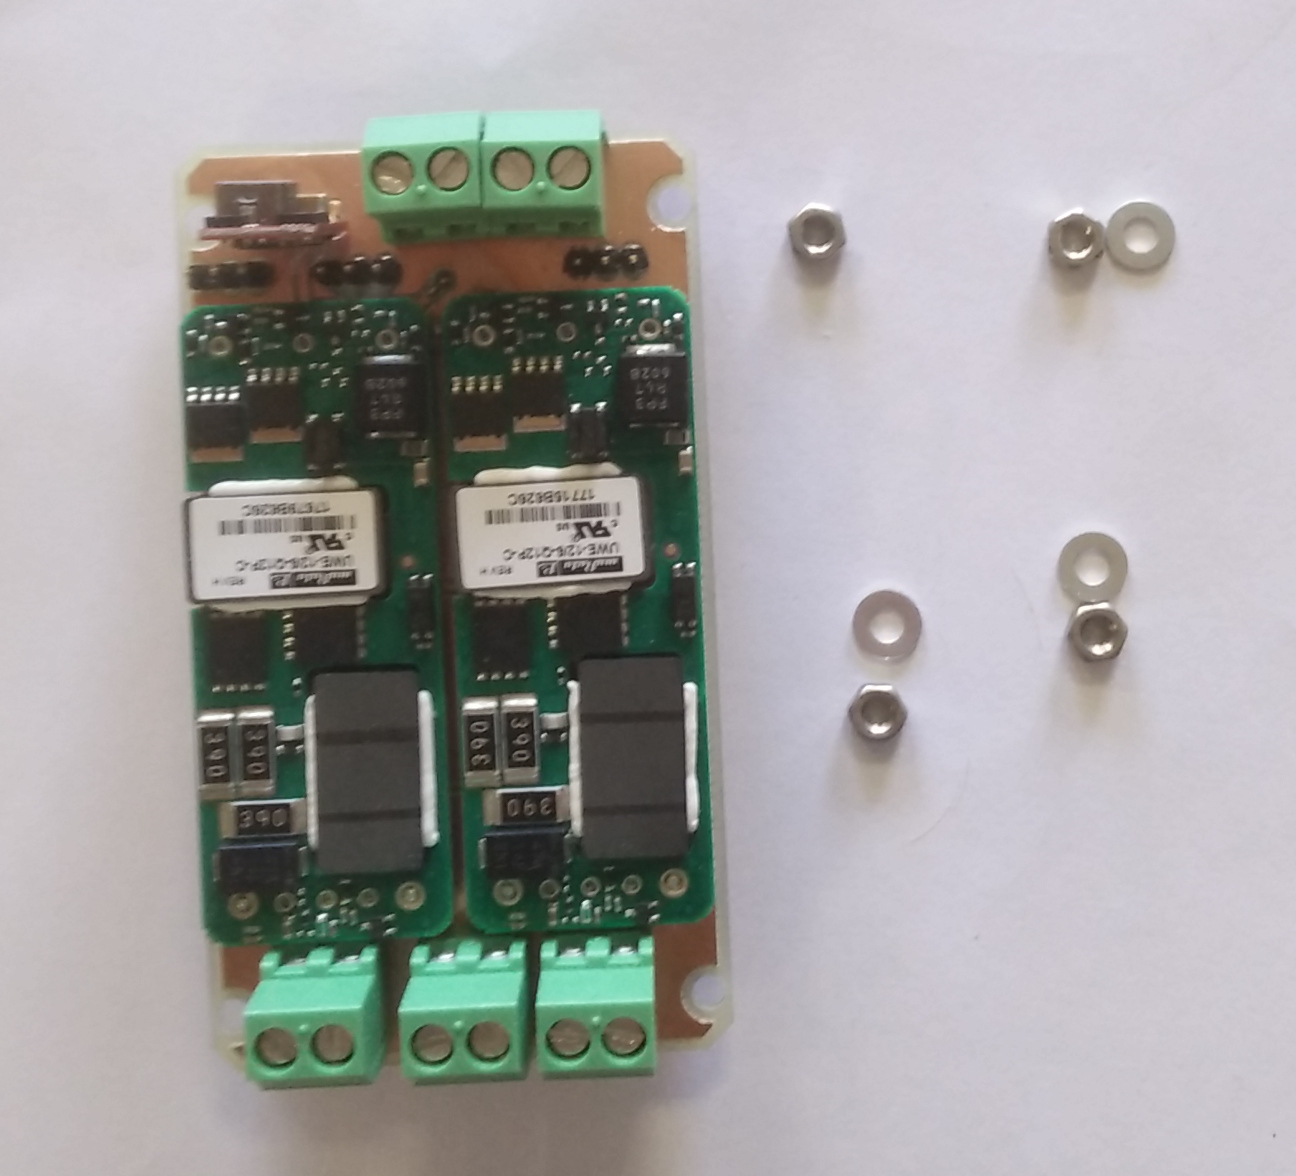
\includegraphics[width=150px]{images/23.jpg}
\caption{Components for the power board.}
\label{fig:23}
\end{figure}

\begin{figure}[H]
\center

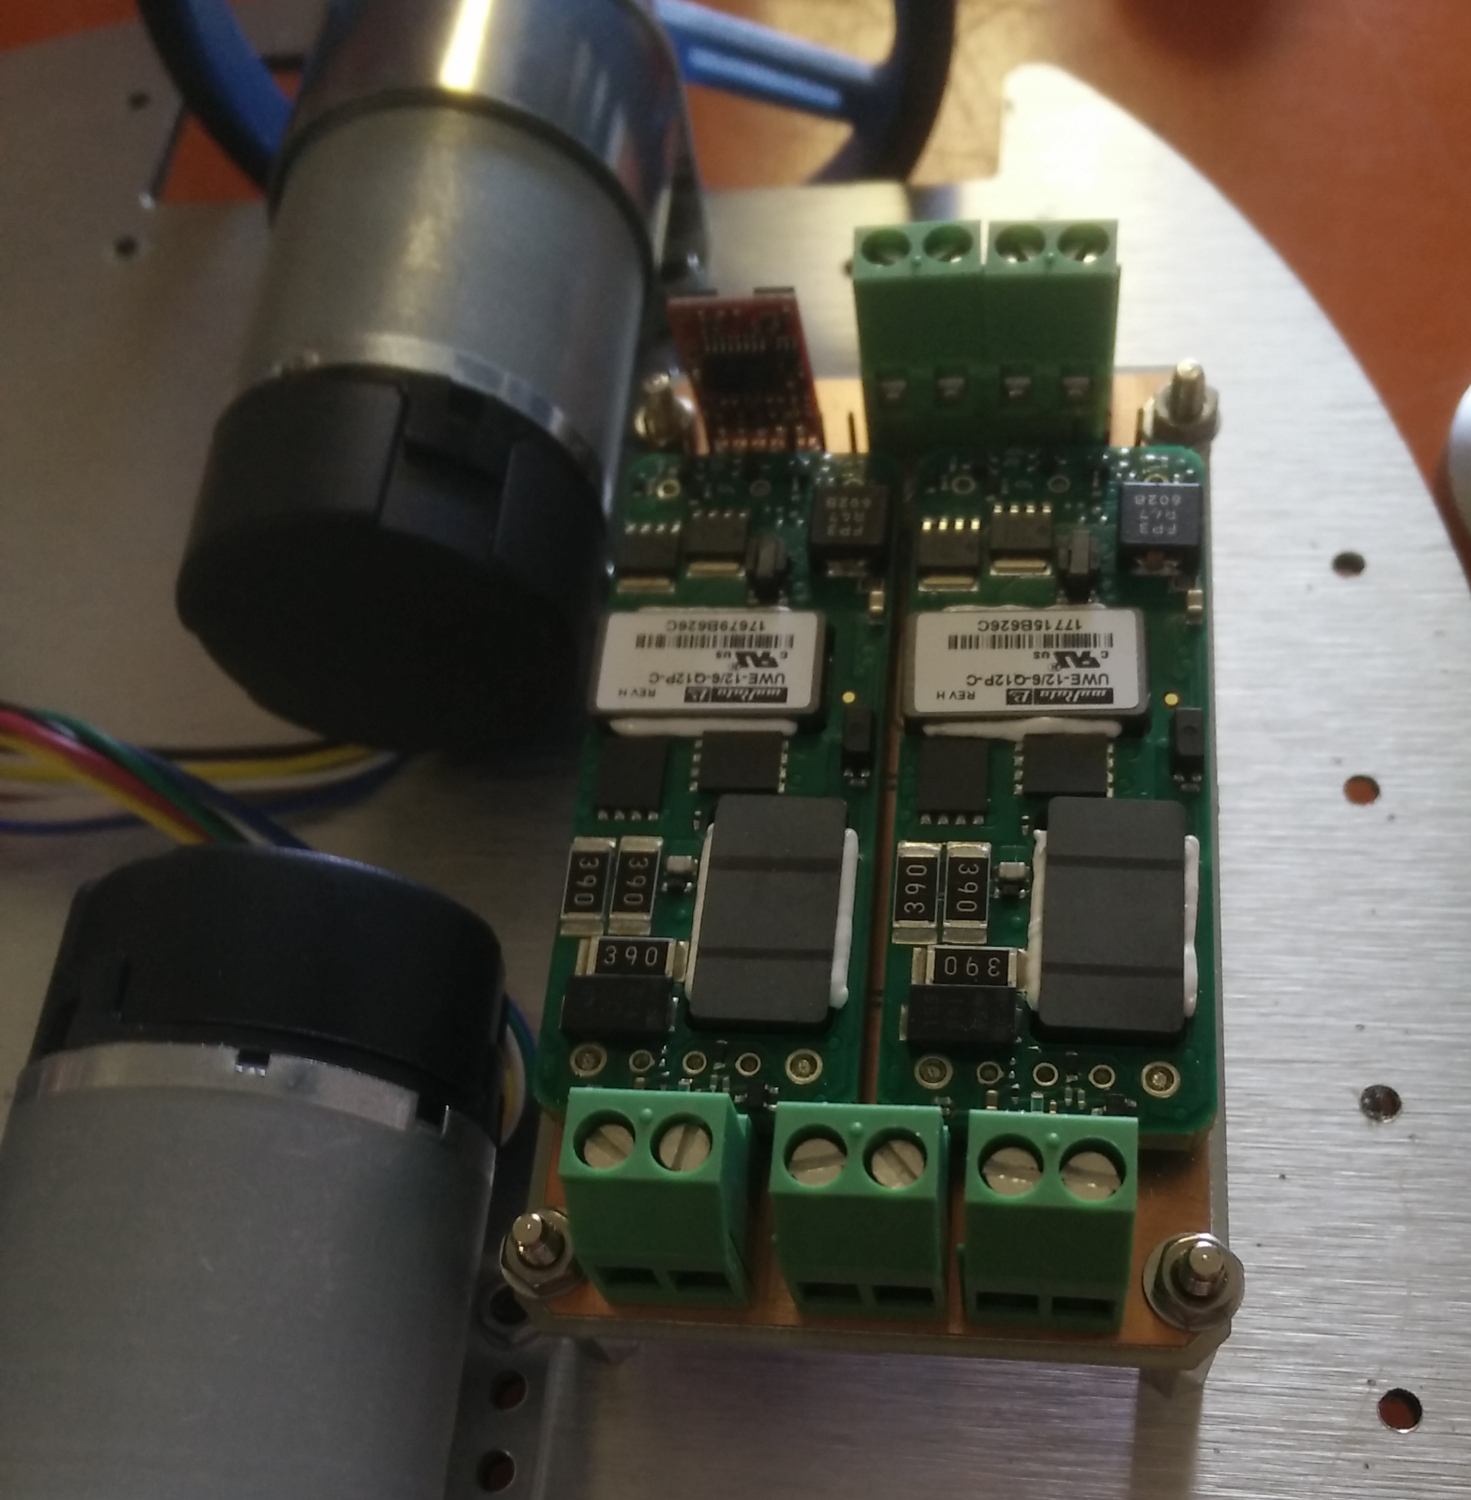
\includegraphics[width=150px]{images/24.jpg}
\caption{The power board in place.}
\label{fig:24}
\end{figure}

\section{Wiring the power board}

To wire the power board, two wires are needed (Figure \ref{fig:25}) : the blue/black one that will be used for connecting the batterie, and the red/black one that will be used to connect the motor boards and the emmergency stop button. \textbf{Be carrefull while connecting those wires} (as connecting the other ones bythe way...)!

\begin{figure}[H]
\center
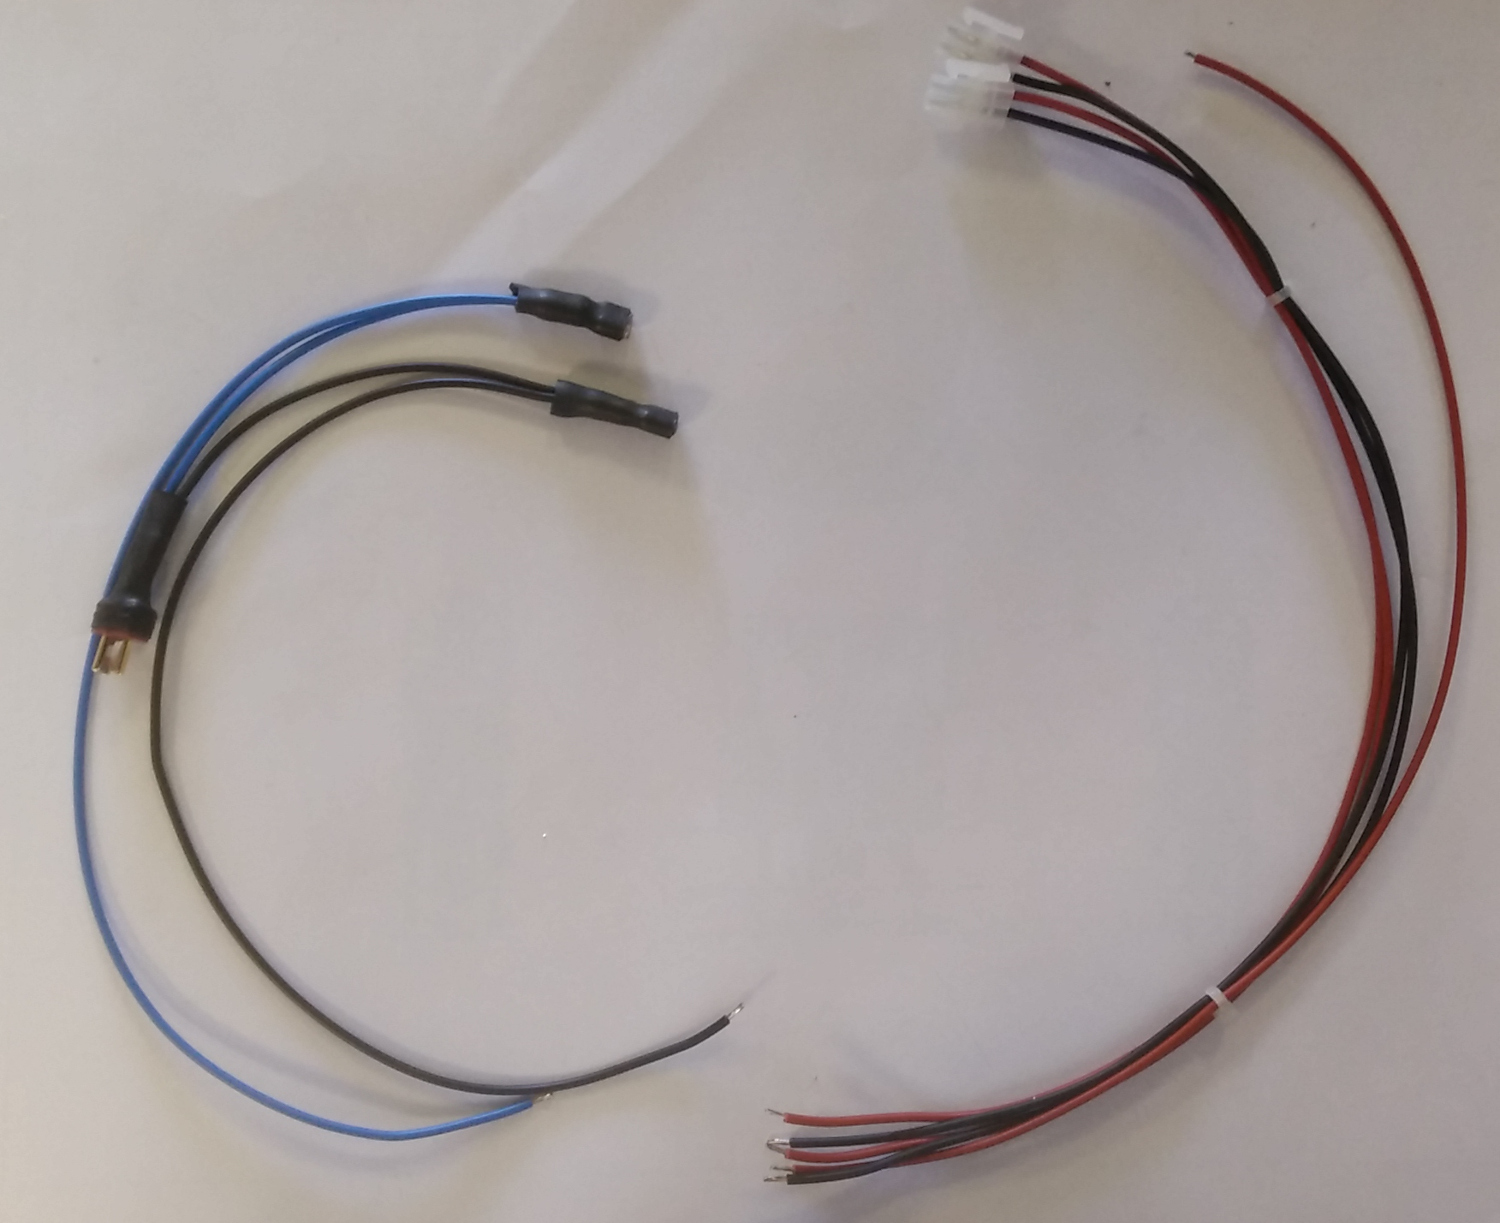
\includegraphics[width=150px]{images/25.jpg}
\caption{Wires for the power board.}
\label{fig:25}
\end{figure}

\subsection{The blue/black wire}

Connect the blue/black wire as depicted in Figure \ref{fig:26}. \textbf{The wire has to go under the board}!

\begin{figure}[H]
\center
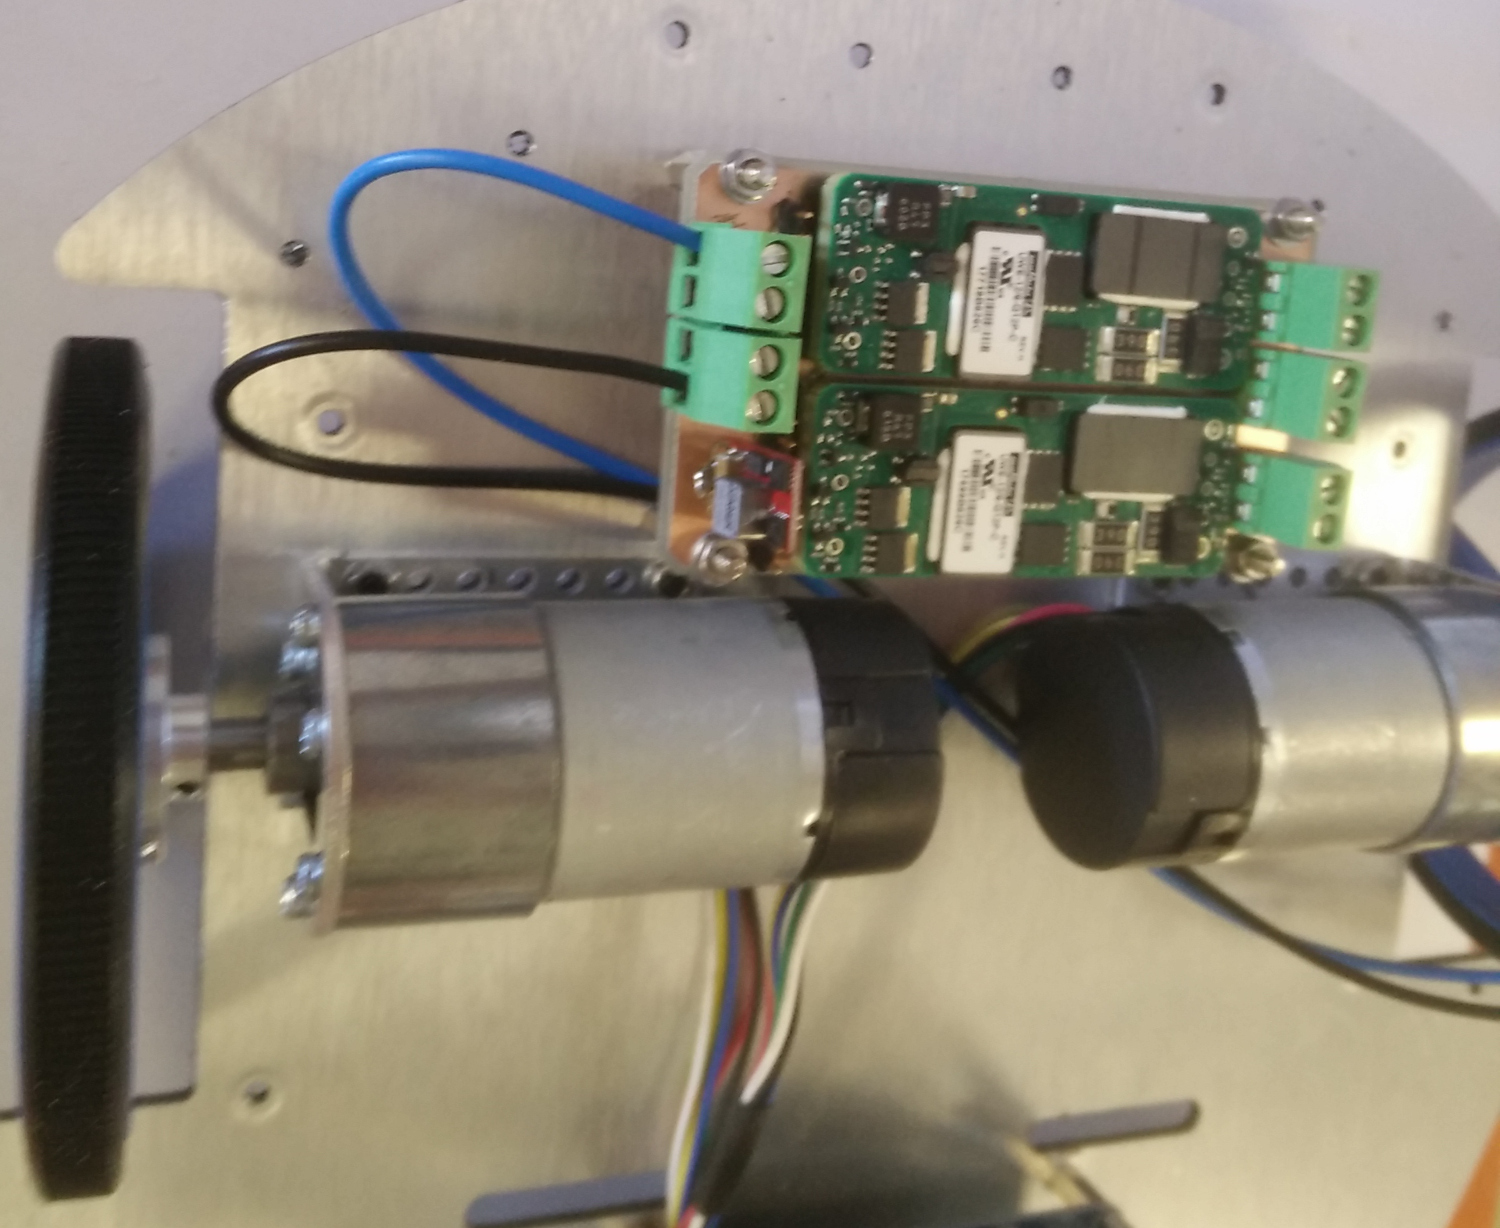
\includegraphics[width=200px]{images/26.jpg}
\caption{Blue/Black wire connection.}
\label{fig:26}
\end{figure}

\subsection{The red/Black wire}

First place the wire under the motor boards as depicted in Figure \ref{fig:27}.
 
\begin{figure}[H]
\center
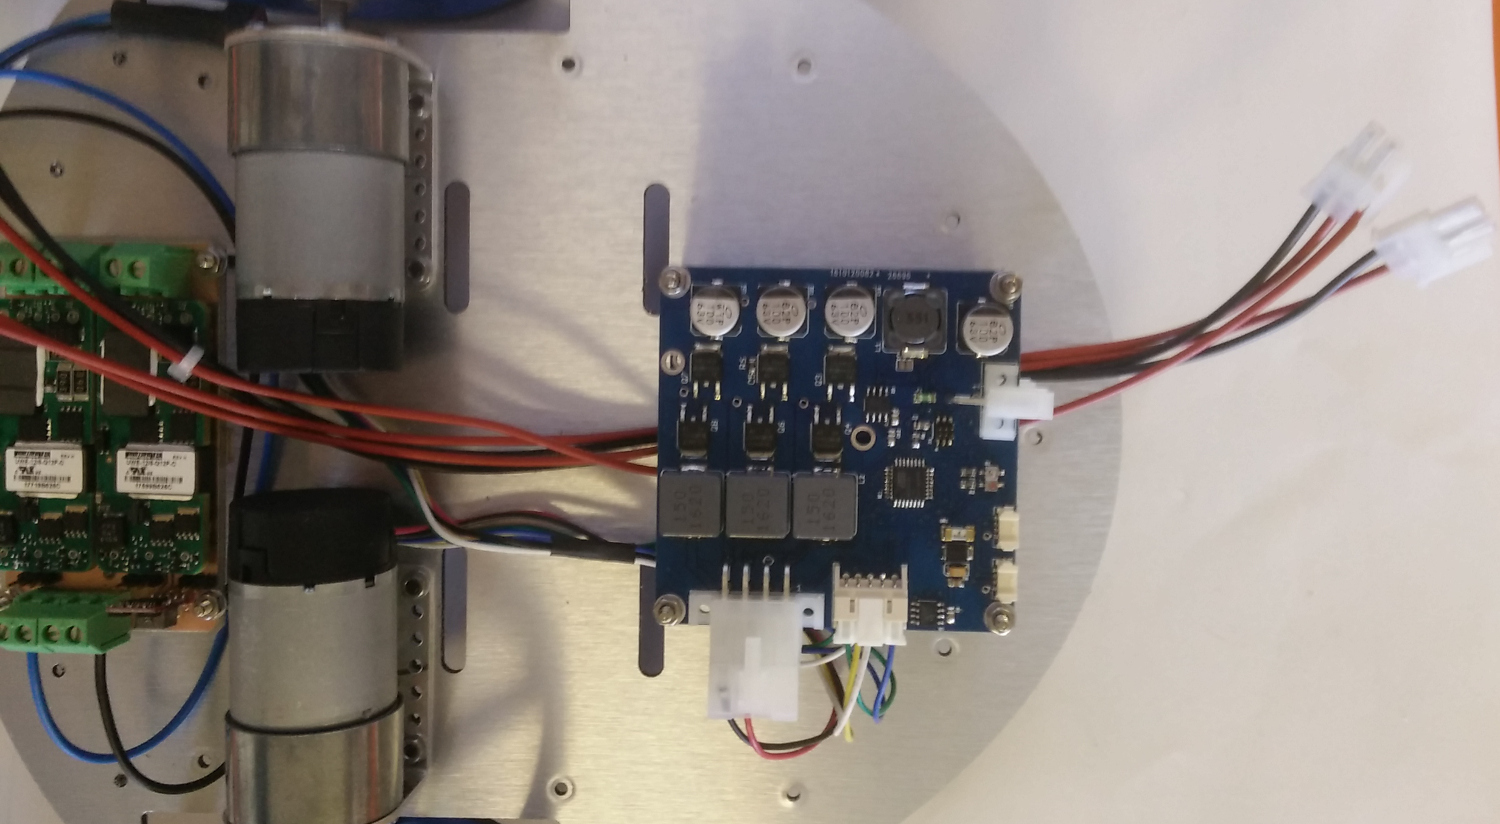
\includegraphics[width=250px]{images/27.jpg}
\caption{Put the wires under the motor boards.}
\label{fig:27}
\end{figure}

Then connect the whites sockets to the motor boards, as illustrated in Figure \ref{fig:28}. 

\begin{figure}[H]
\center
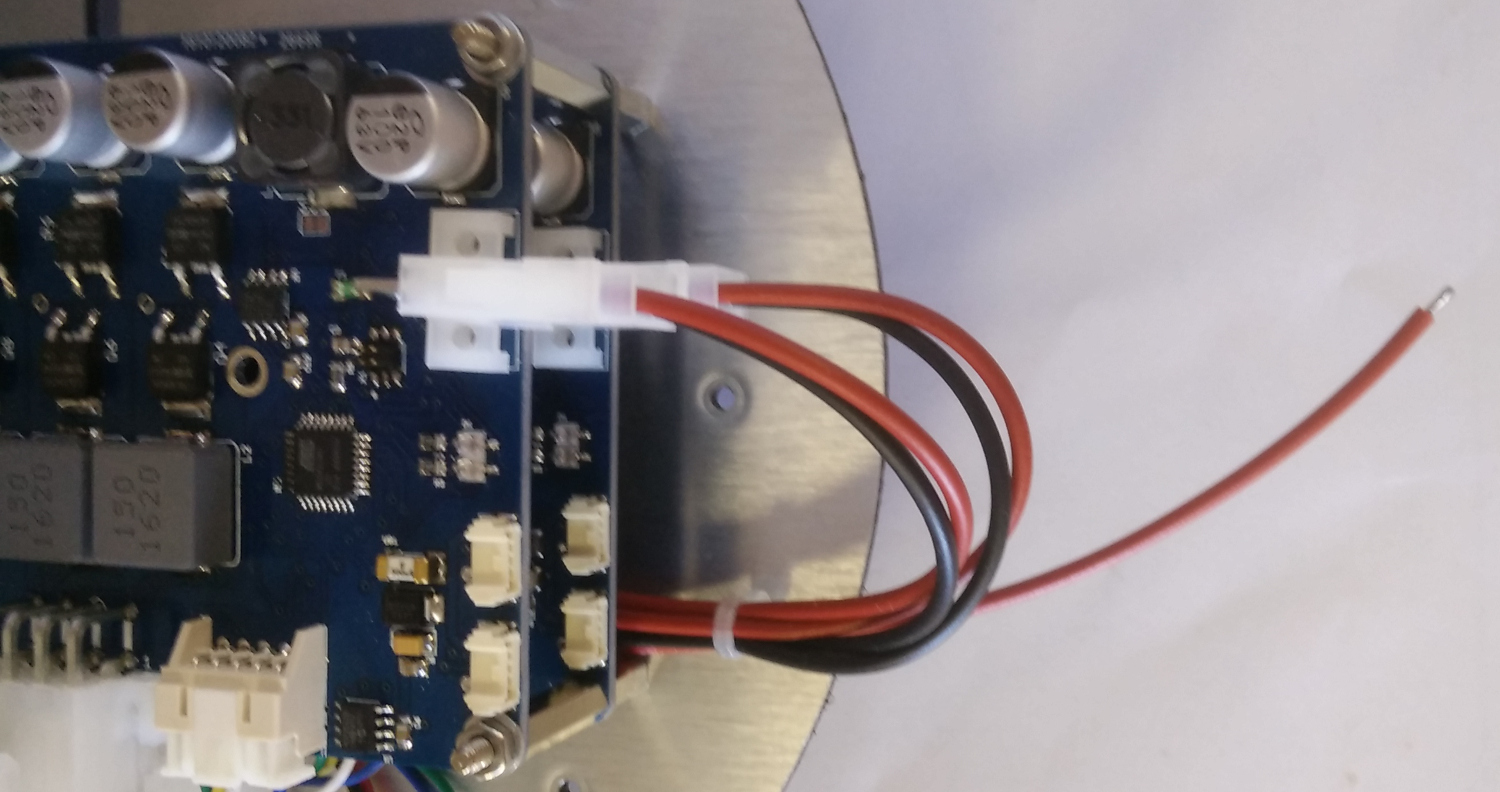
\includegraphics[width=250px]{images/28.jpg}
\caption{Wire to the motor boards.}
\label{fig:28}
\end{figure}

Once the wire is connected to the motor boards, put it in the same configuration as presented in Figure \ref{fig:29}, in order to dissociate the "lonely" red wire and the blacks ends, to the red ends.
\begin{figure}[H]
\center
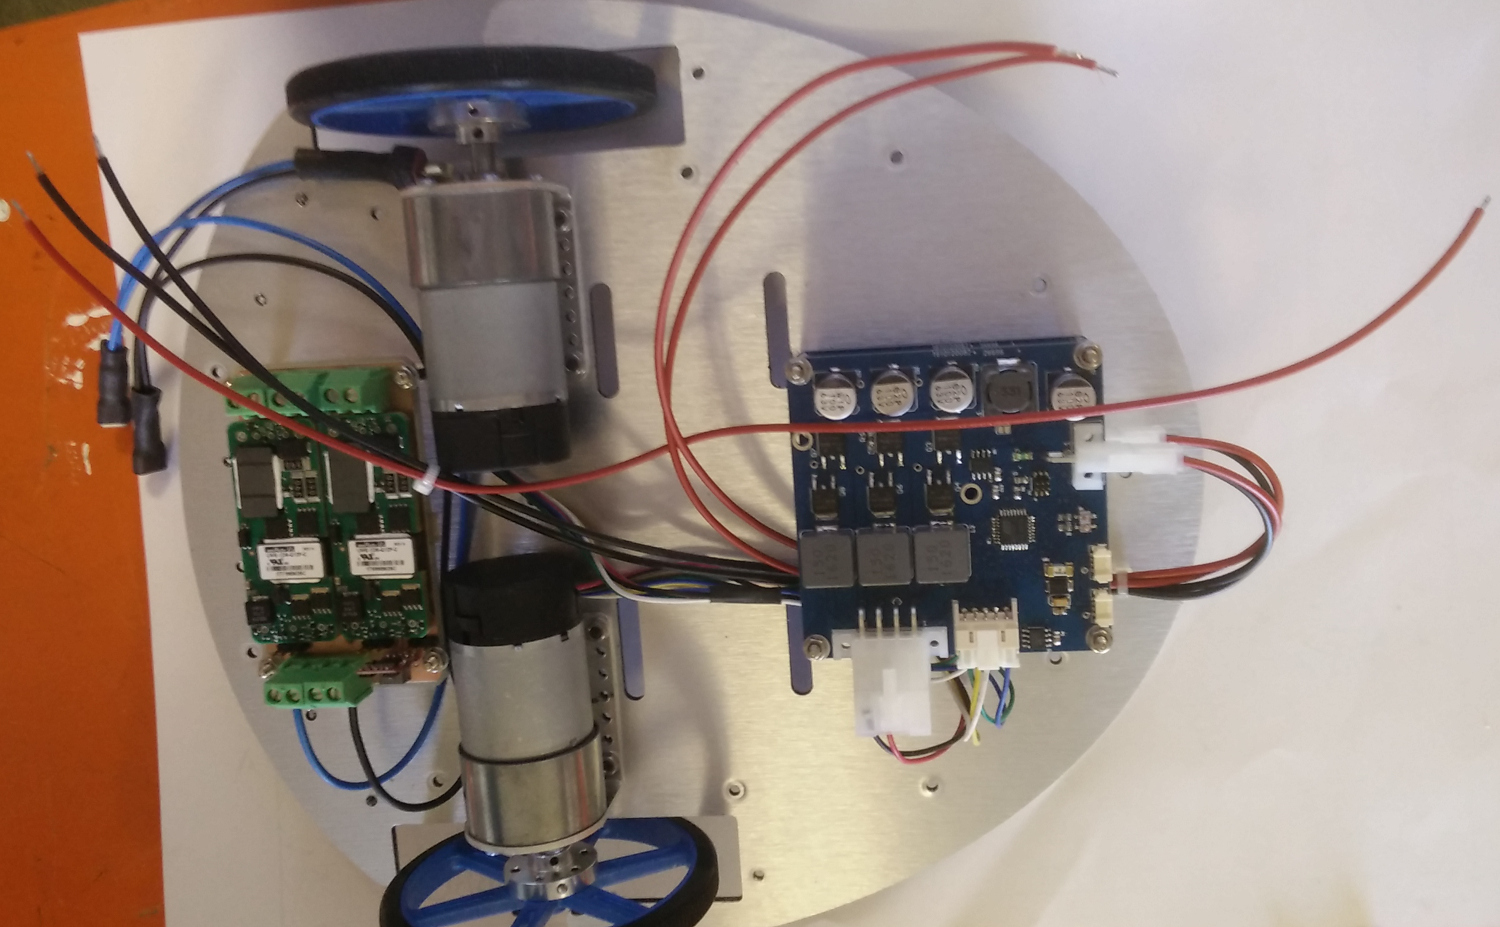
\includegraphics[width=250px]{images/29.jpg}
\caption{Identify the red/black wire extremities.}
\label{fig:29}
\end{figure}

 Once you have identified the black ends end the lonely red, put them under the power board as illustrated in Figure \ref{fig:30}. 

\begin{figure}[H]
\center
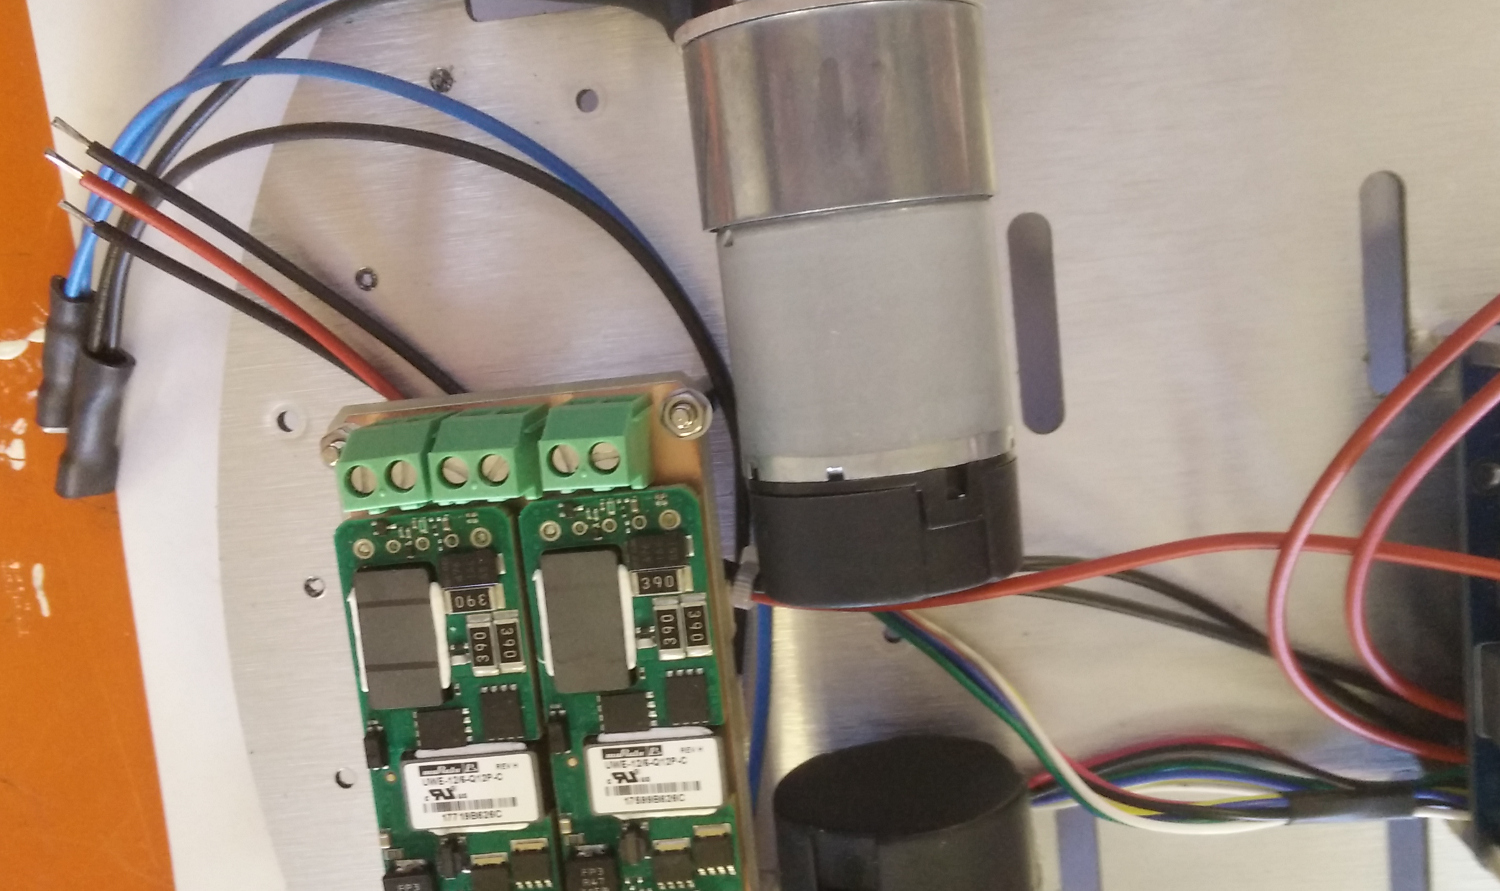
\includegraphics[width=250px]{images/30.jpg}
\caption{Put the wires under the power board.}
\label{fig:30}
\end{figure}

Connect the black extremities as depicted in Figure \ref{fig:31}.

\begin{figure}[H]
\center
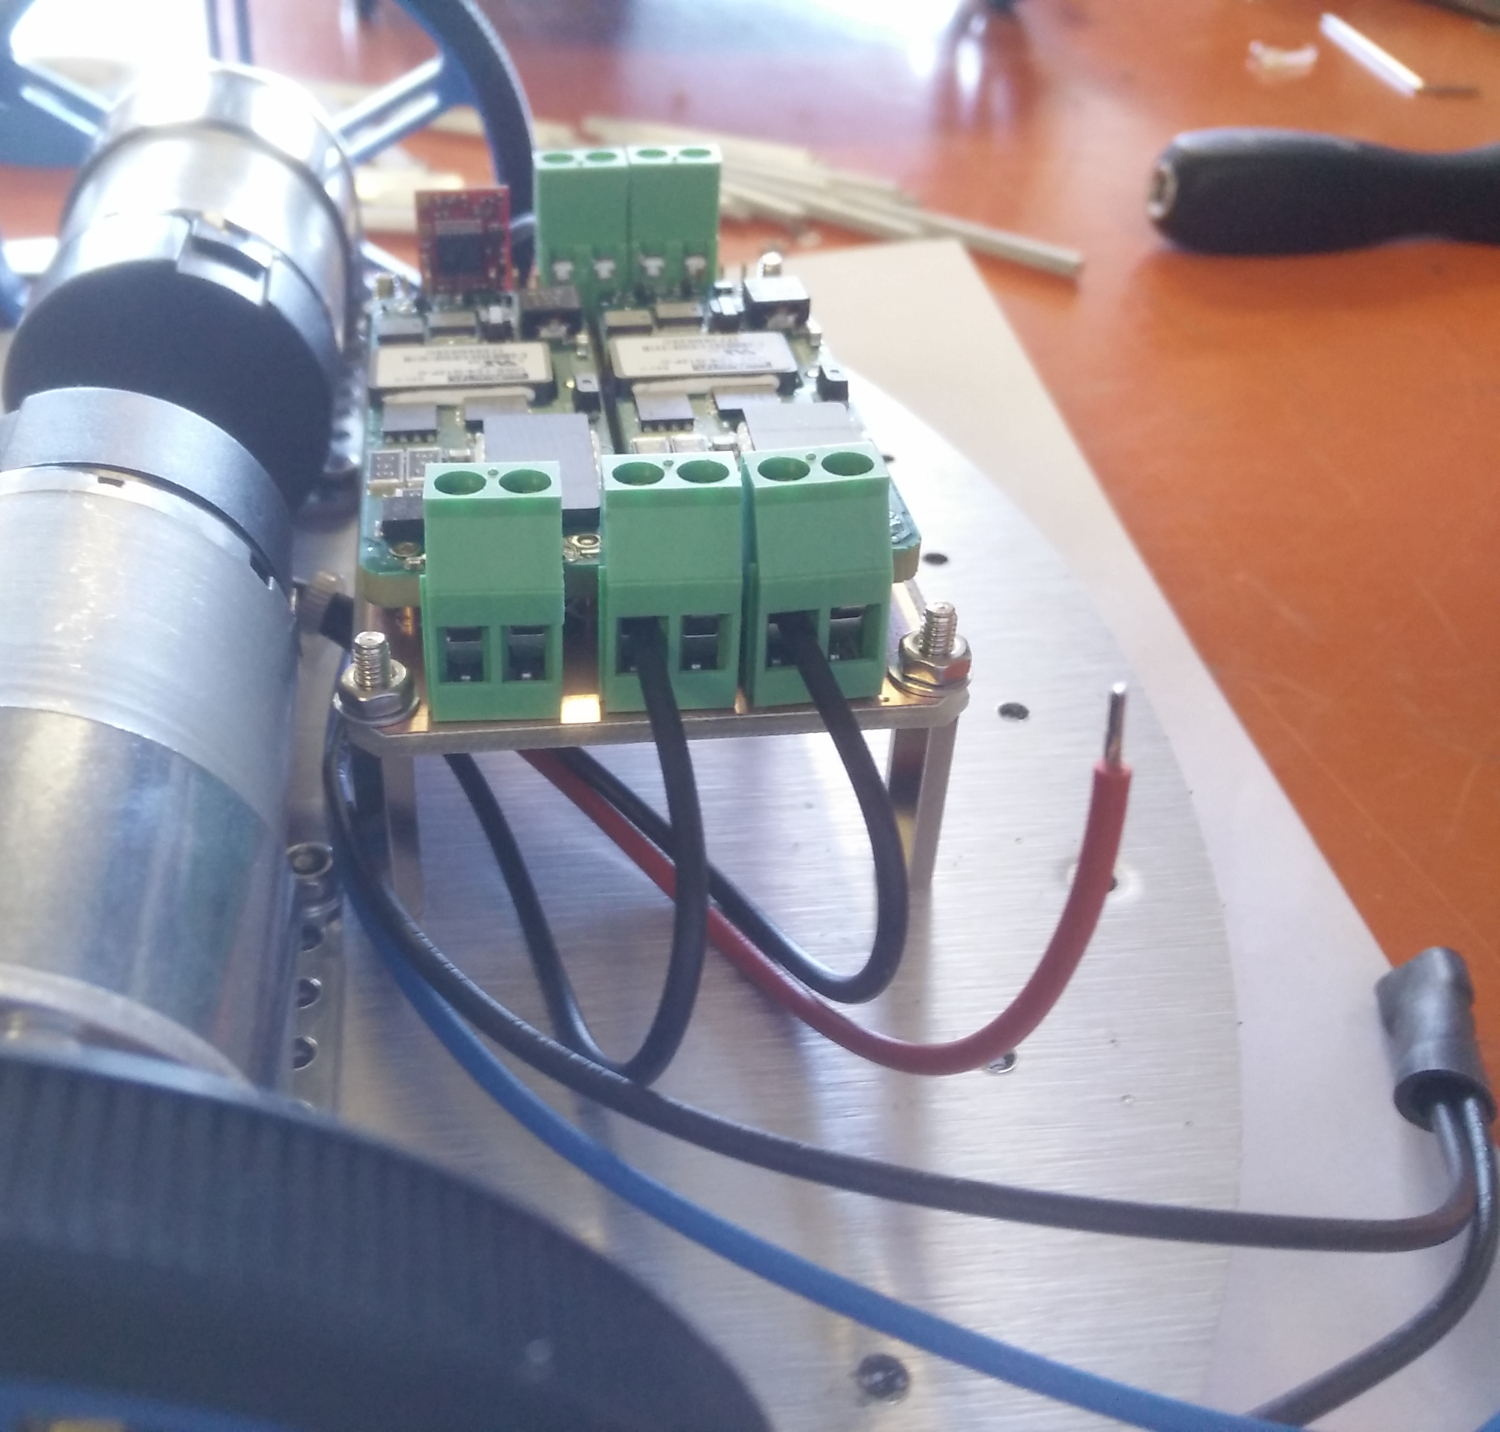
\includegraphics[width=200px]{images/31.jpg}
\caption{Connect the black wires.}
\label{fig:31}
\end{figure}

 Finally, take a small red wire (left part of Figure \ref{fig:32}) and wire the red wires as presented in Figure \ref{fig:32}.

\begin{figure}[H]
\center
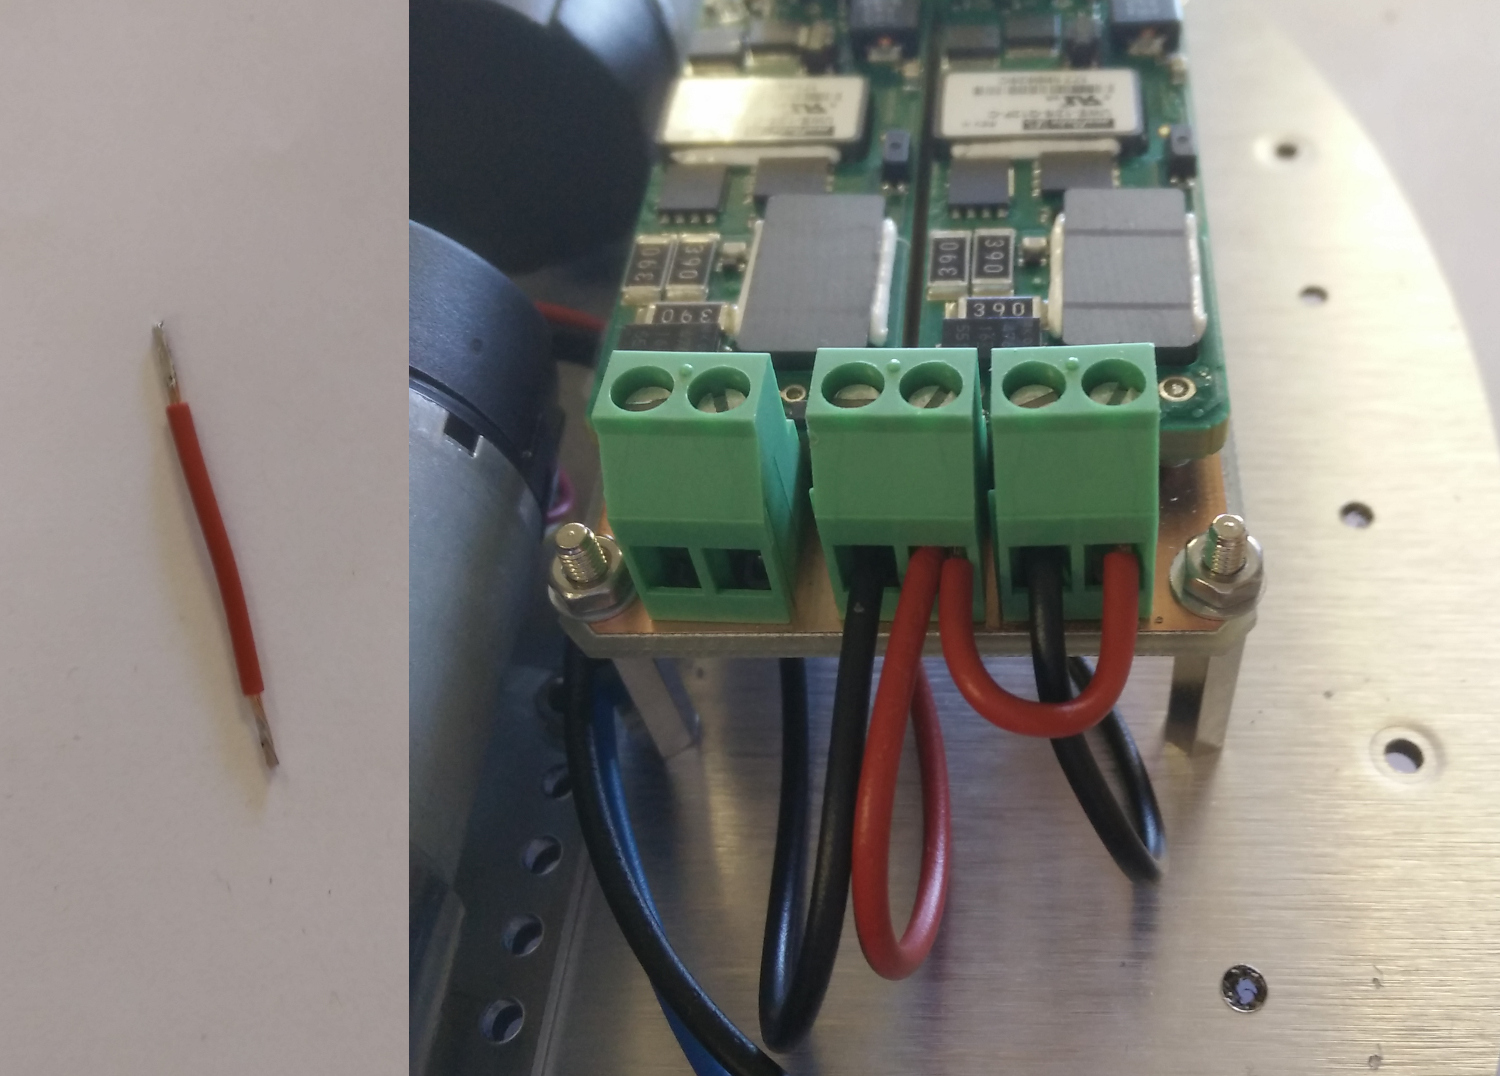
\includegraphics[width=250px]{images/32.jpg}
\caption{Connect the red wires.}
\label{fig:32}
\end{figure}

\section{The CAN/Bus wiring: motor boards to power board}

The communication inside the robot is done through a CAN bus. It exists height different wires inside the IstiaBot, as depicted in Figure \ref{fig:33}. \textbf{Warning: the blue and red wires are not switchable, as the blues are direct wires while the reds are crossed wires}. For the wires with the same colors, only the lengths of the wires change.

\begin{figure}[H]
\center
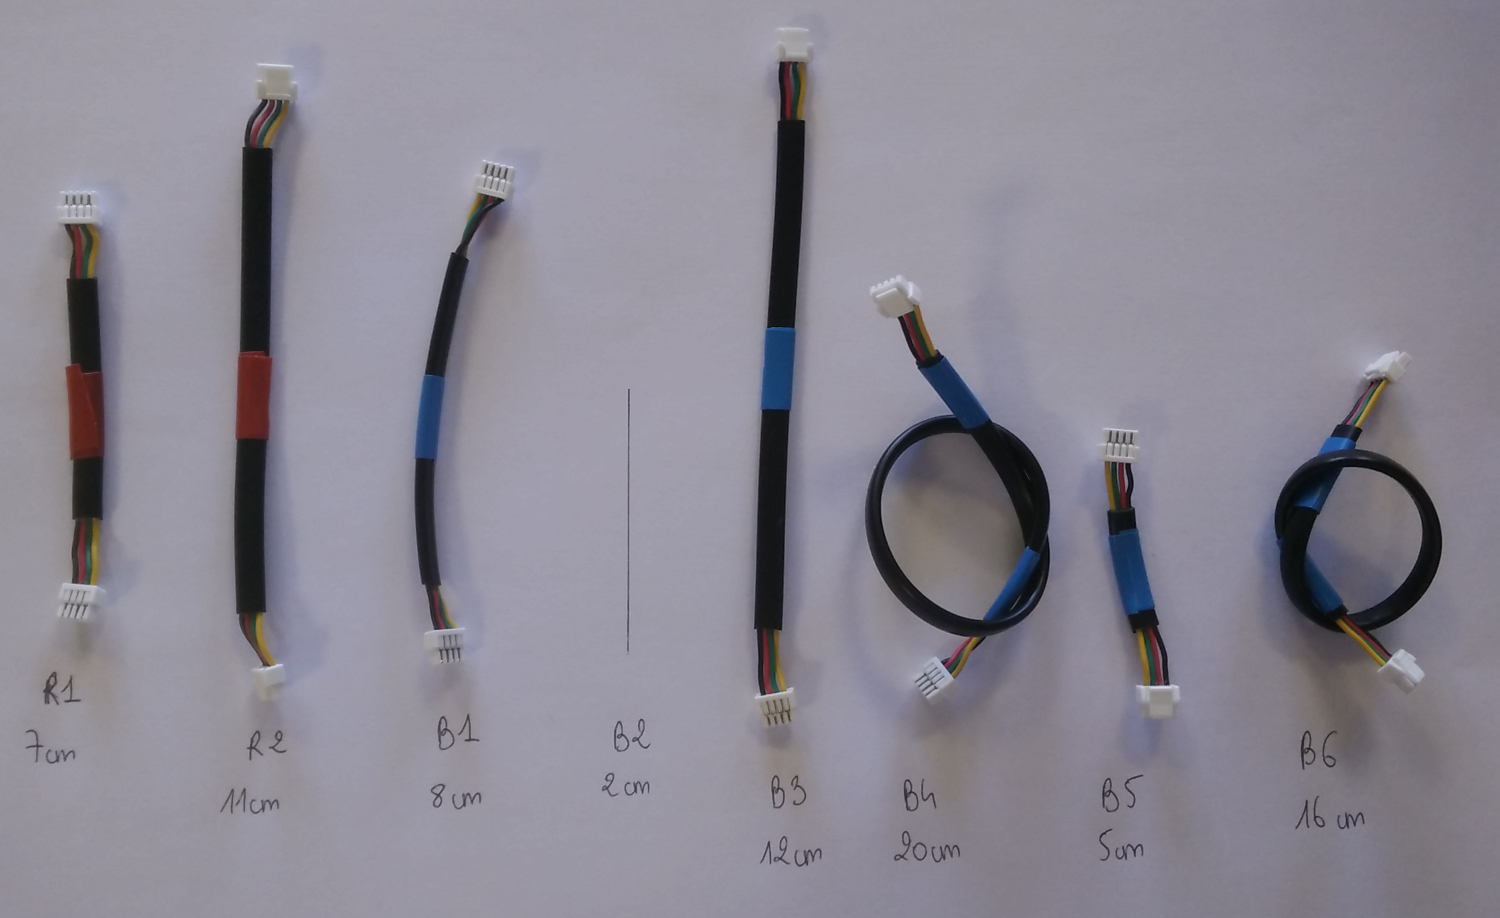
\includegraphics[width=350px]{images/33.jpg}
\caption{The different CAN wires.}
\label{fig:33}
\end{figure}

The first CAN wire to put, is the B5 (blue, 5cm) wire between the two motor boards, as depicted in Figure \ref{fig:34}.

\begin{figure}[H]
\center
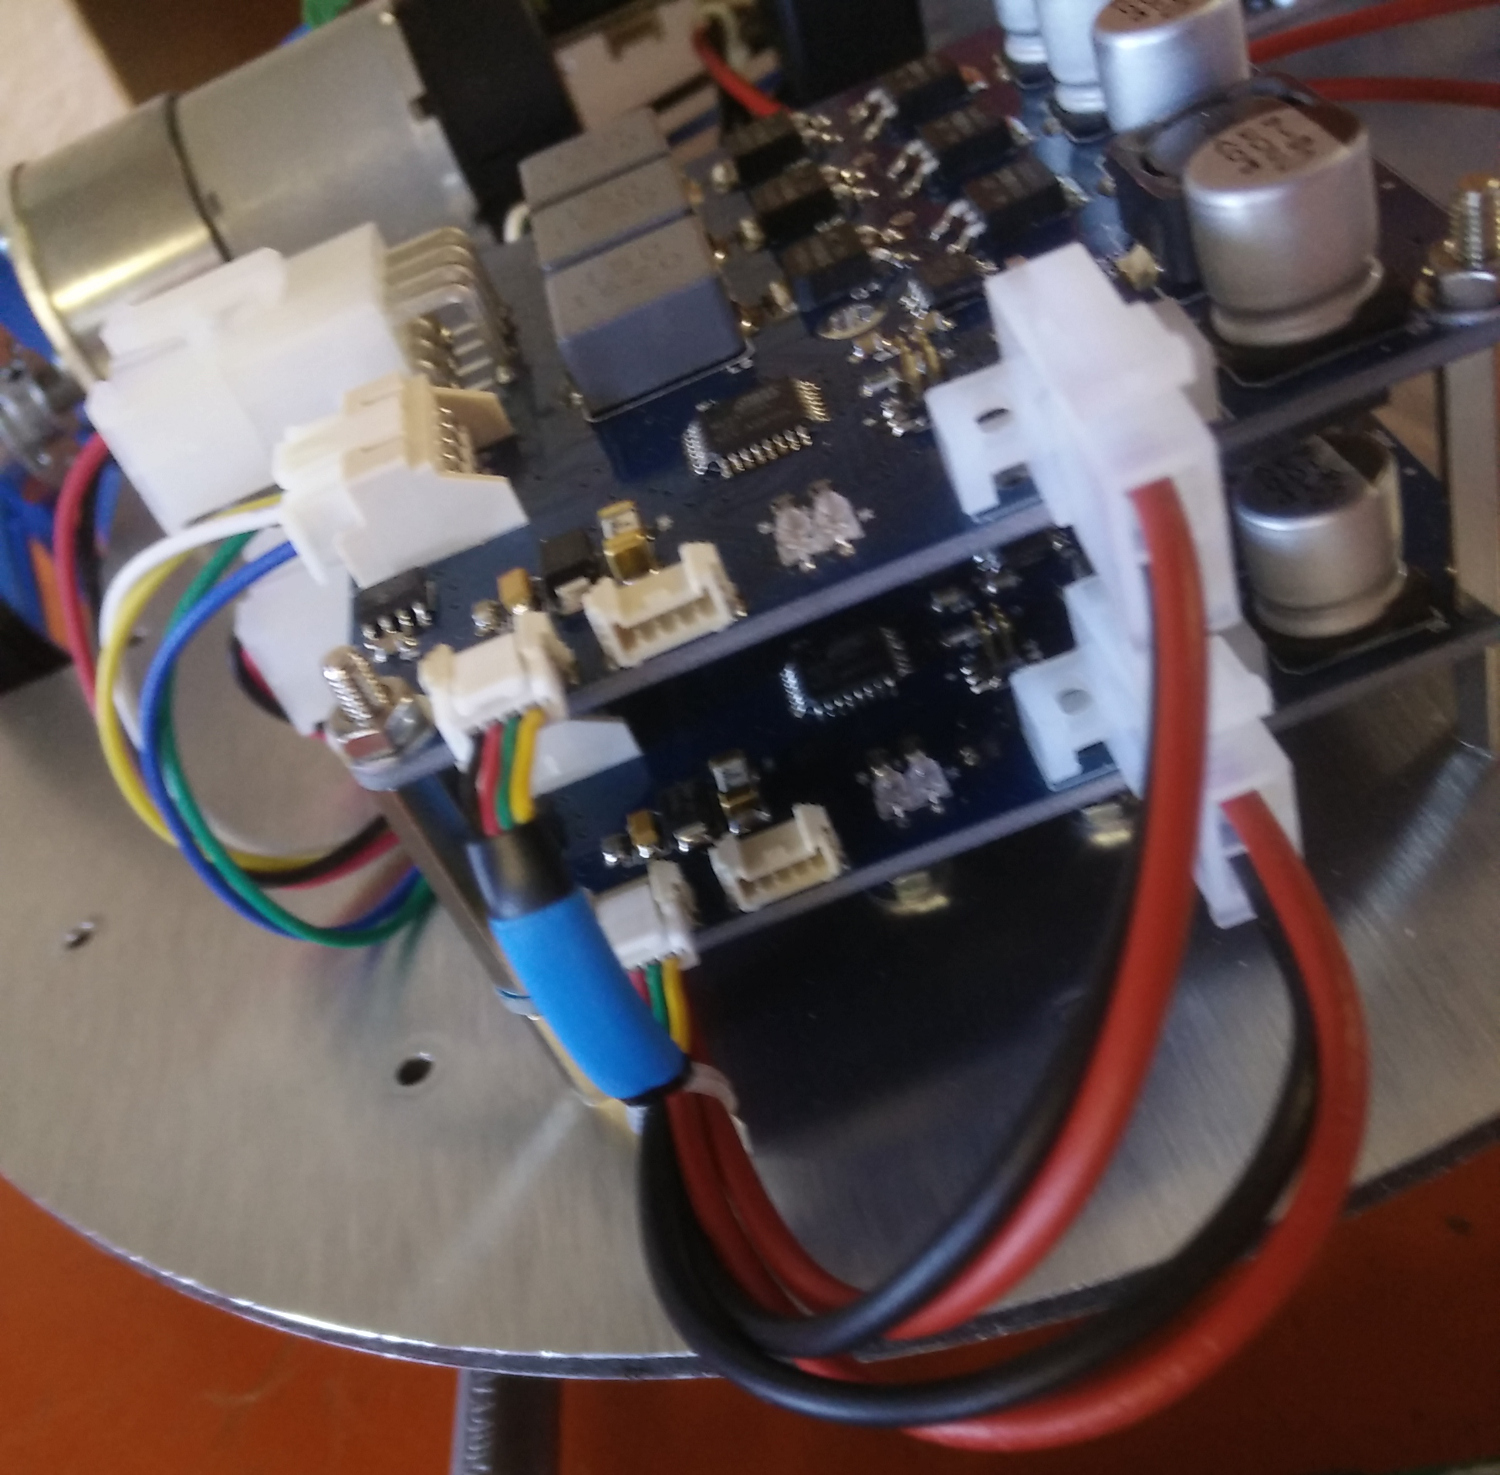
\includegraphics[width=200px]{images/34.jpg}
\caption{CAN bus between the motor boards.}
\label{fig:34}
\end{figure}

Then it is needed to connect the motor boards to the power board, by using a B6 wire (Blue, 16cm). \textbf{Note that the wire goes under the motor boards}, as depicted in Figure \ref{fig:35}.

\begin{figure}[H]
\center
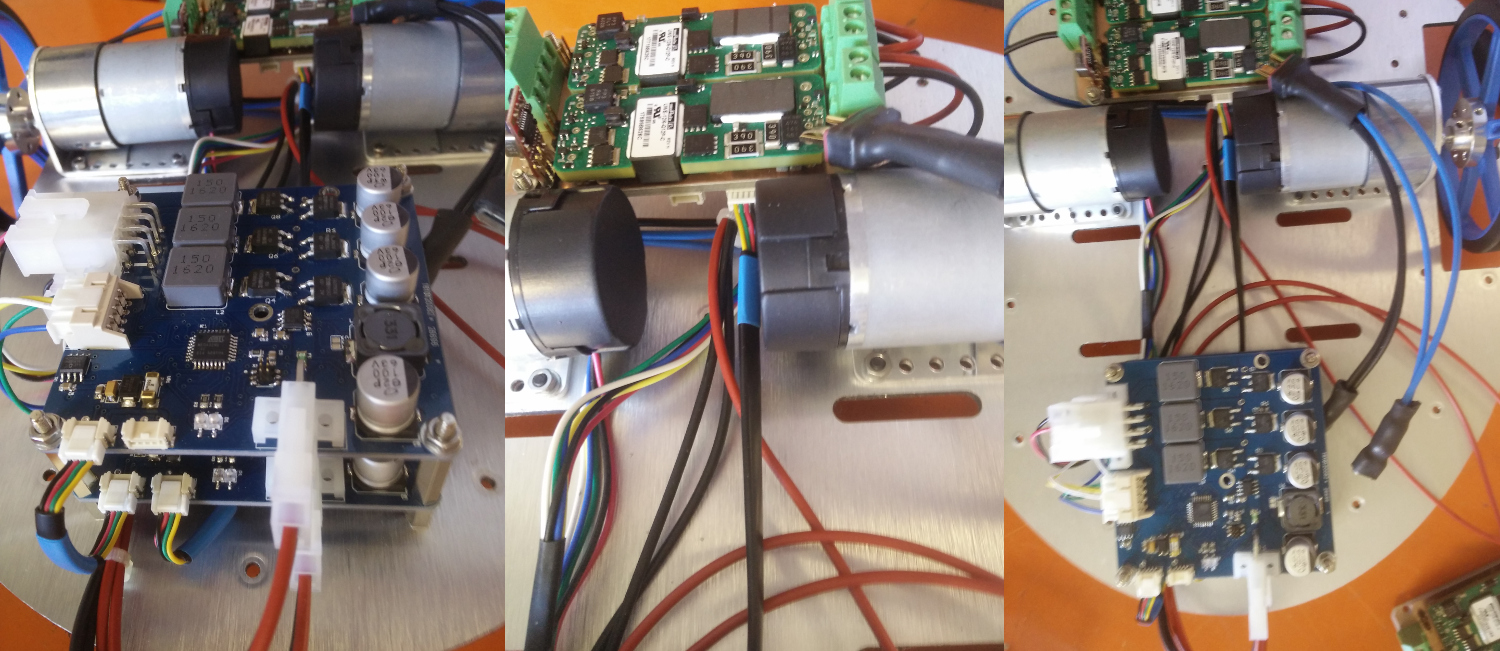
\includegraphics[width=350px]{images/35.jpg}
\caption{CAN bus between the motor boards and the power board.}
\label{fig:35}
\end{figure}

\section{The CAN/Bus wiring: ultra-sounds}

The next step is to install the ultra-sounds sensors. It is easier to wire the US before placing them on the plate. Connect a R1 wire (Red, 7cm) to the top of the first US, then a B1 wire (Blue, 8cm) to the bottom of the first and the bottom of the double US. Use a B3 wire (Blue, 12 cm) to connect the top of the double sensor with the top of the fourth one. And finally connect a R2 wire (Red, 11 cm) to the bottom of the last US sensor. Figure \ref{fig:36} details this wiring. Note that the wire between the double sensors (B2, blue 2cm) is already in place, \textbf{do not remove it}!

\begin{figure}[H]
\center
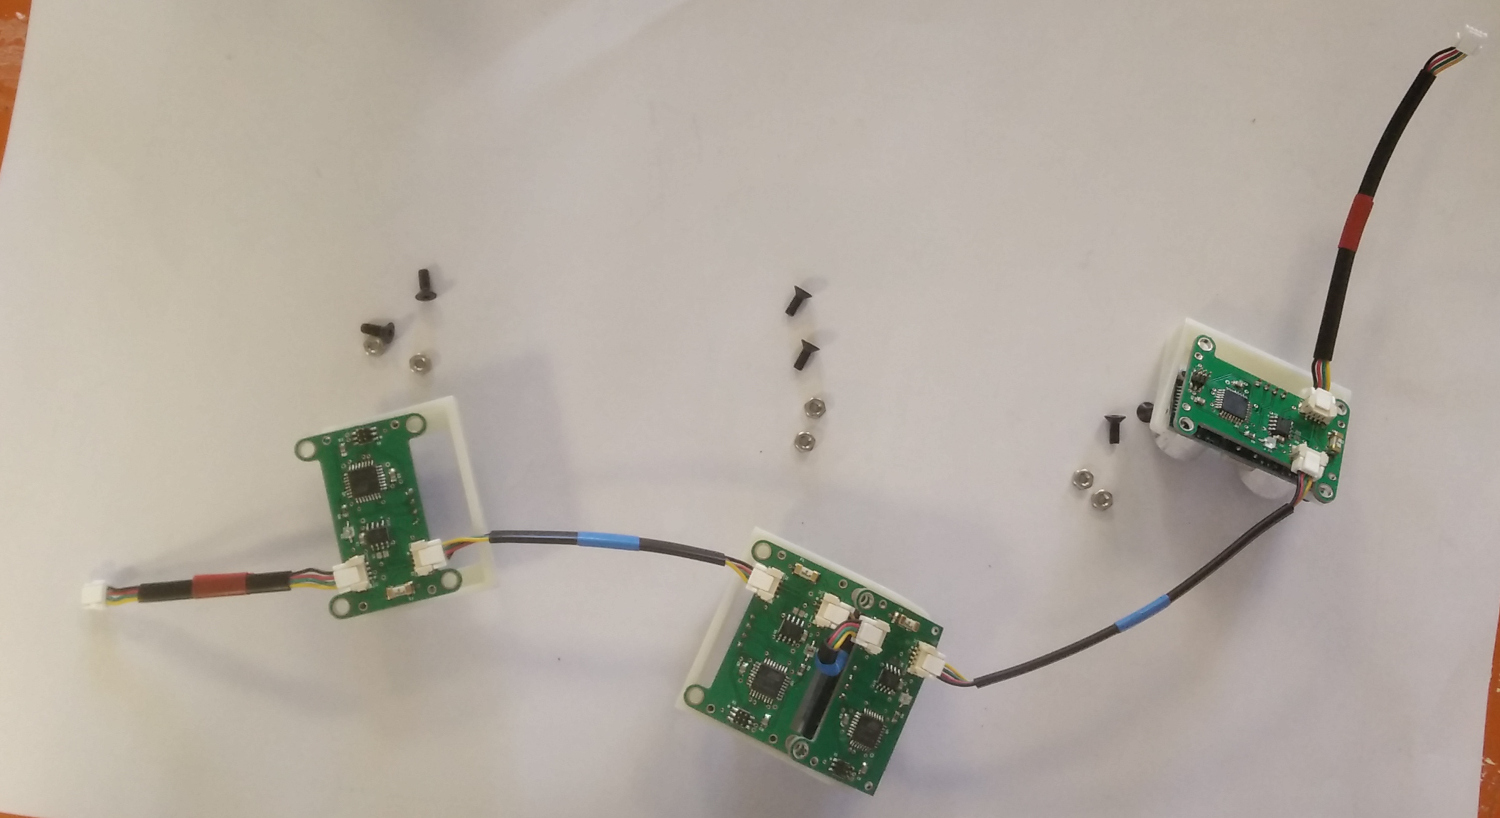
\includegraphics[width=300px]{images/36.jpg}
\caption{CAN bus between the Utra-Sound sensors.}
\label{fig:36}
\end{figure}

Connect the last sensor (R2 wire) with the power board, as depicted in Figure \ref{fig:37}. \textbf{Put the wire under the power board!} 

\begin{figure}[H]
\center
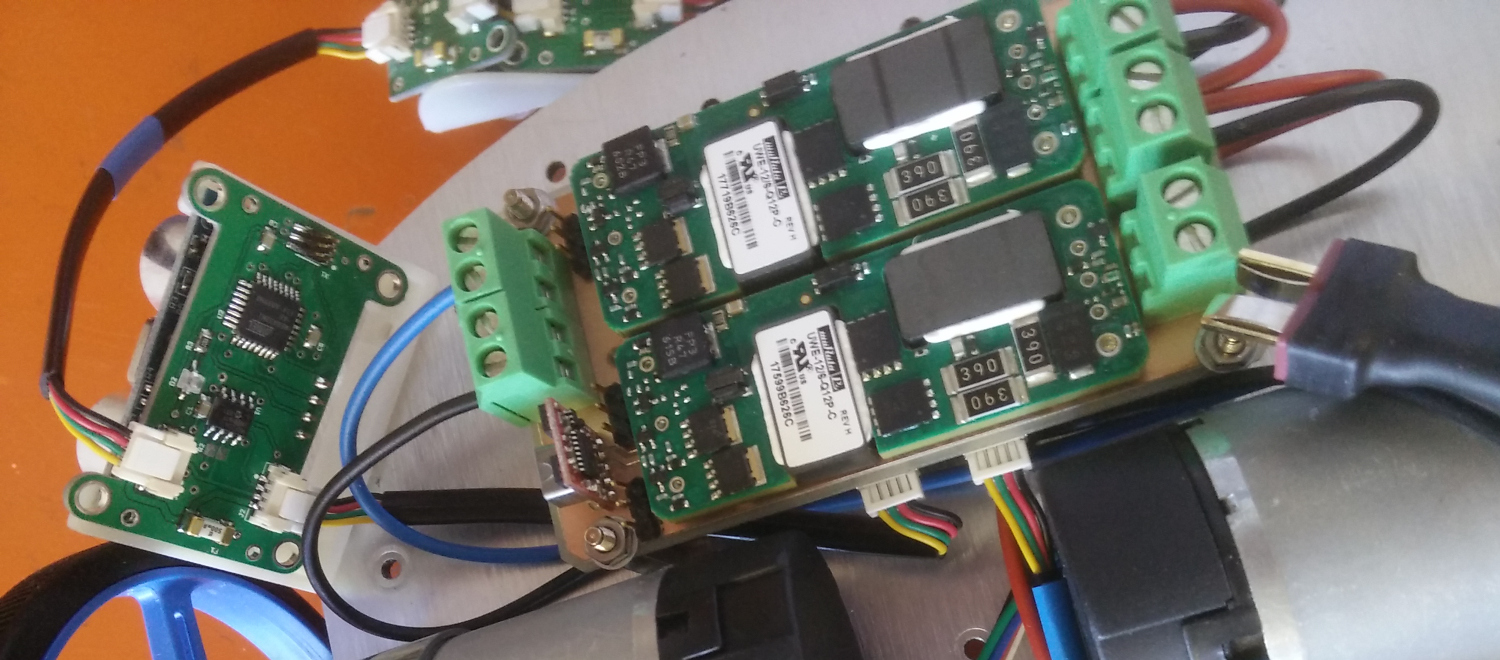
\includegraphics[width=300px]{images/37.jpg}
\caption{CAN bus between the Utra-Sound and the power board.}
\label{fig:37}
\end{figure}

Then screw the sensor as depicted in Figure \ref{fig:38}.

\begin{figure}[H]
\center
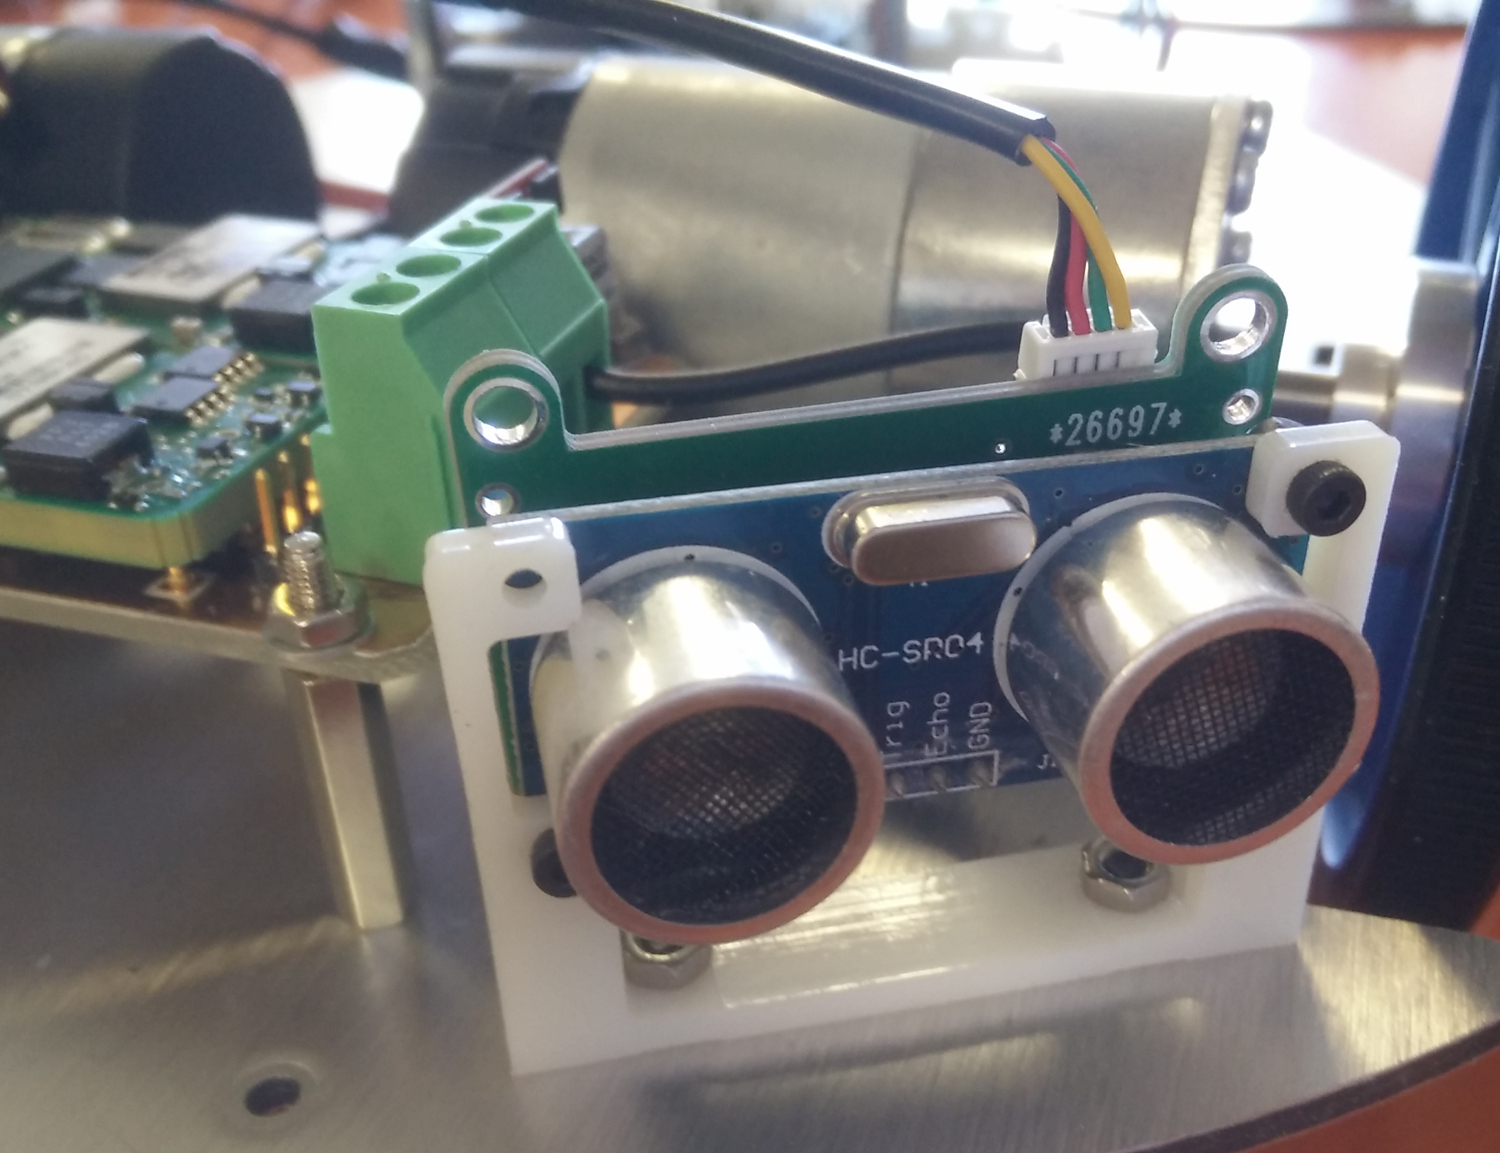
\includegraphics[width=150px]{images/38.jpg}
\caption{Fixing the first US to the plate.}
\label{fig:38}
\end{figure}

Before fixing the others ultra-sound sensors, you need to place the wire B1 \textbf{under the power board}, as depicted in Figure \ref{fig:39}.

\begin{figure}[H]
\center
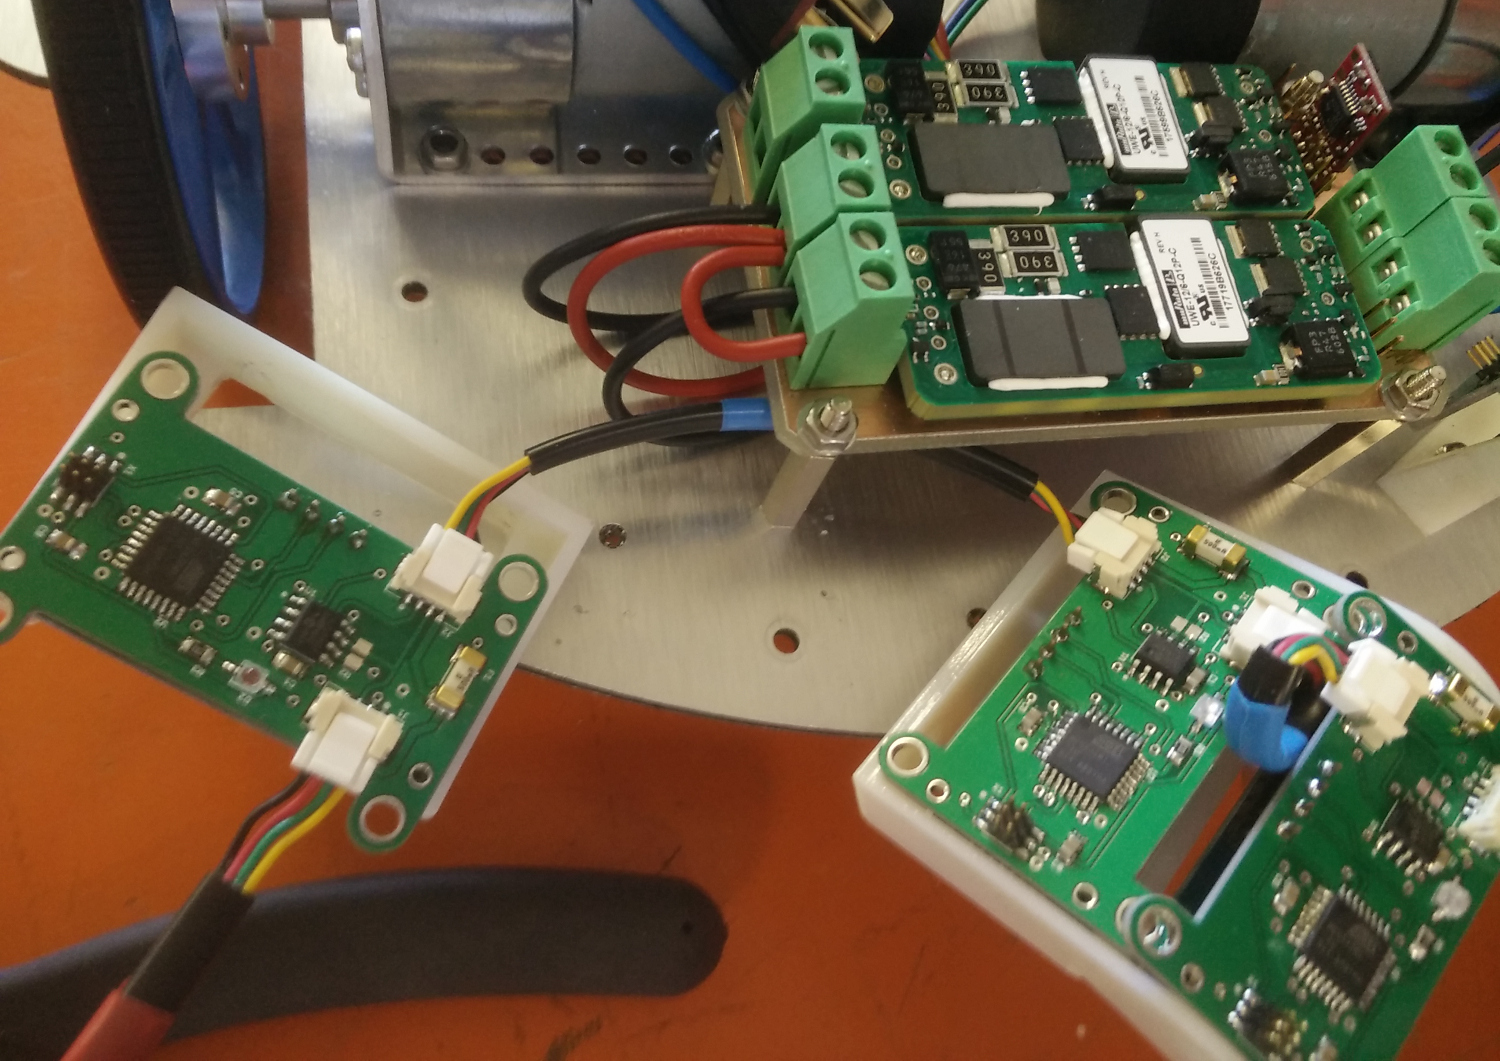
\includegraphics[width=200px]{images/39.jpg}
\caption{Placing the wire under the power board.}
\label{fig:39}
\end{figure}

Finally it is possible to screw the lasts US sensors as depicted in Figure \ref{fig:40}.

\begin{figure}[H]
\center
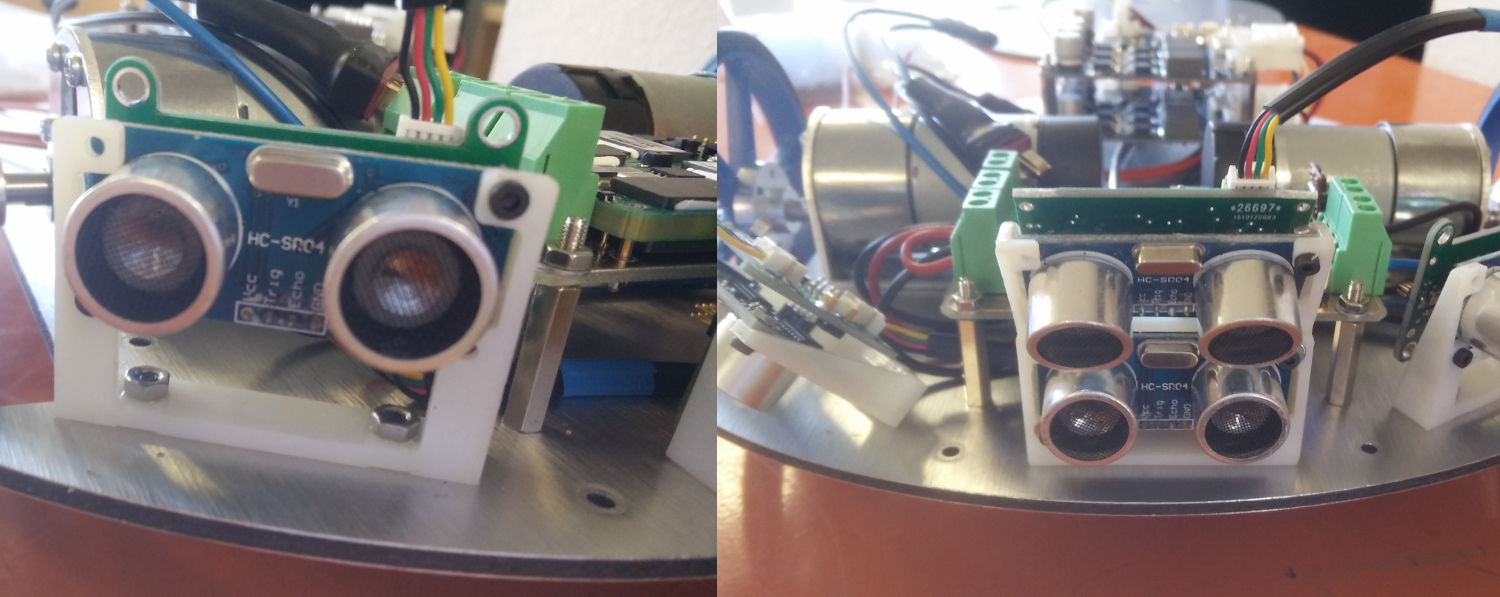
\includegraphics[width=300px]{images/40.jpg}
\caption{Fixing the lasts US.}
\label{fig:40}
\end{figure}

 You should now have the result presented in Figure \ref{fig:41}.

\begin{figure}[H]
\center
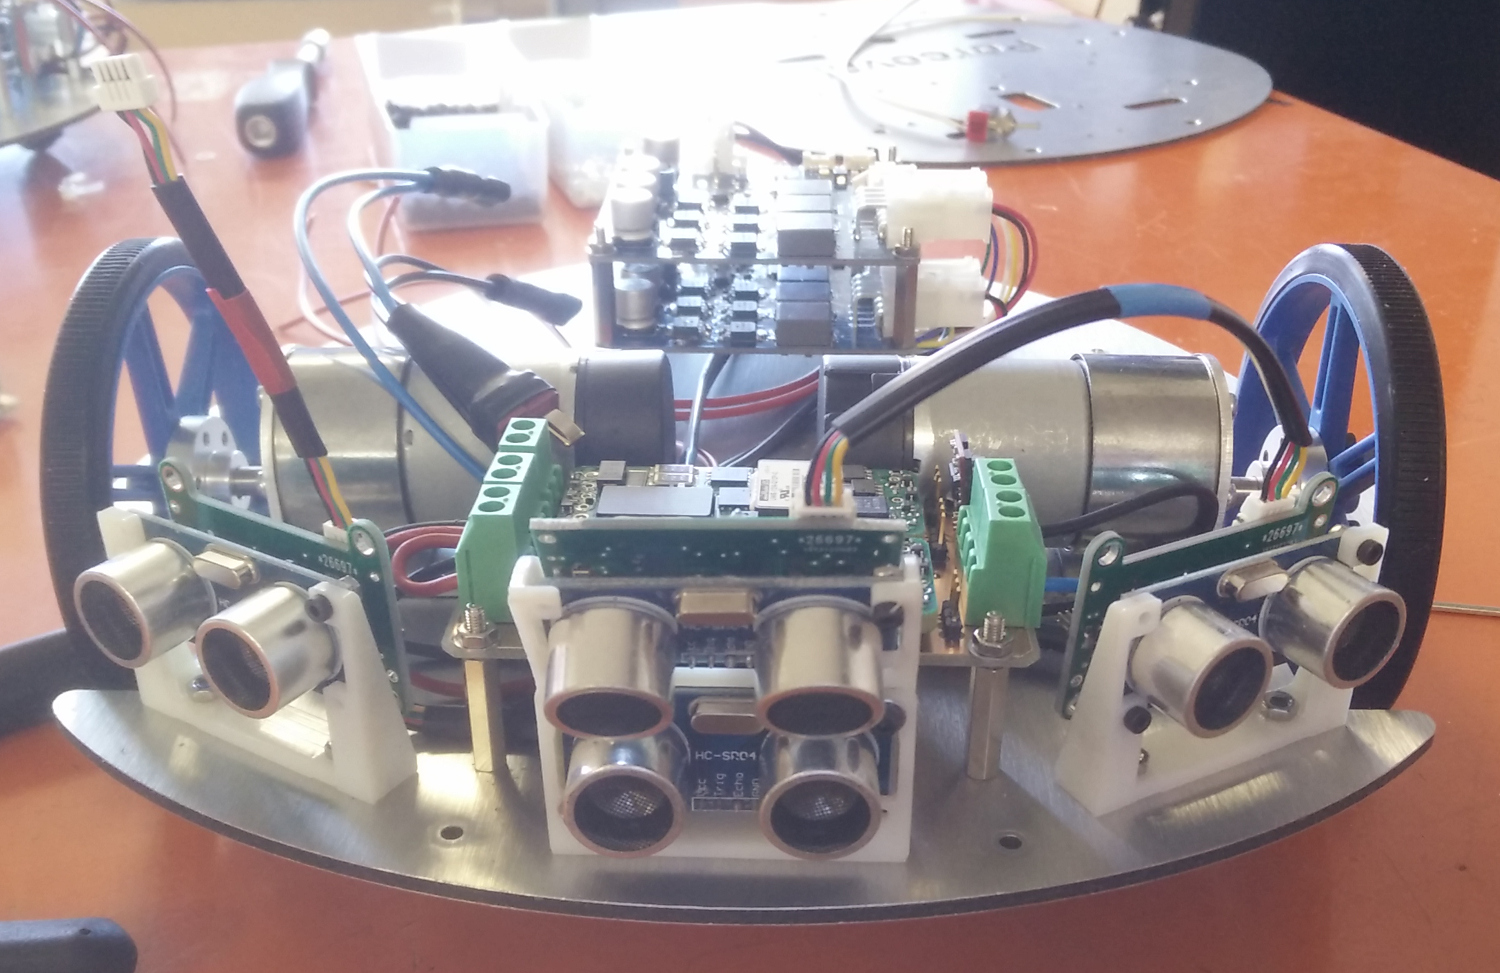
\includegraphics[width=250px]{images/41.jpg}
\caption{Result with the US.}
\label{fig:41}
\end{figure}

\section{The ON/OFF switch}

The next step is to wire the ON/OFF switch. The needed wire is depicted in Figure \ref{fig:42}. 

\begin{figure}[H]
\center
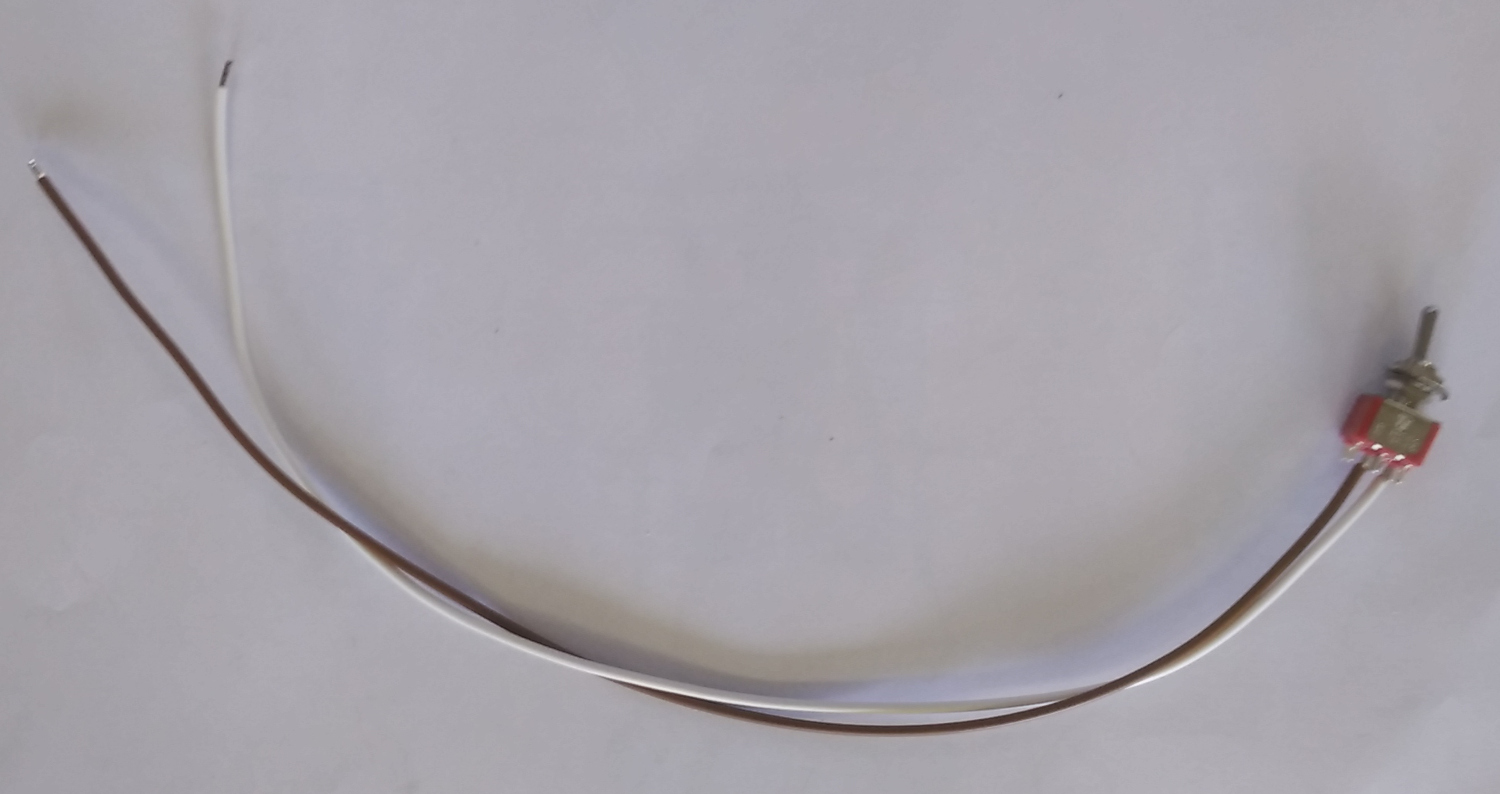
\includegraphics[width=250px]{images/42.jpg}
\caption{The switch component.}
\label{fig:42}
\end{figure}

Put the wire under the power board as depicted in Figure \ref{fig:43}.

\begin{figure}[H]
\center
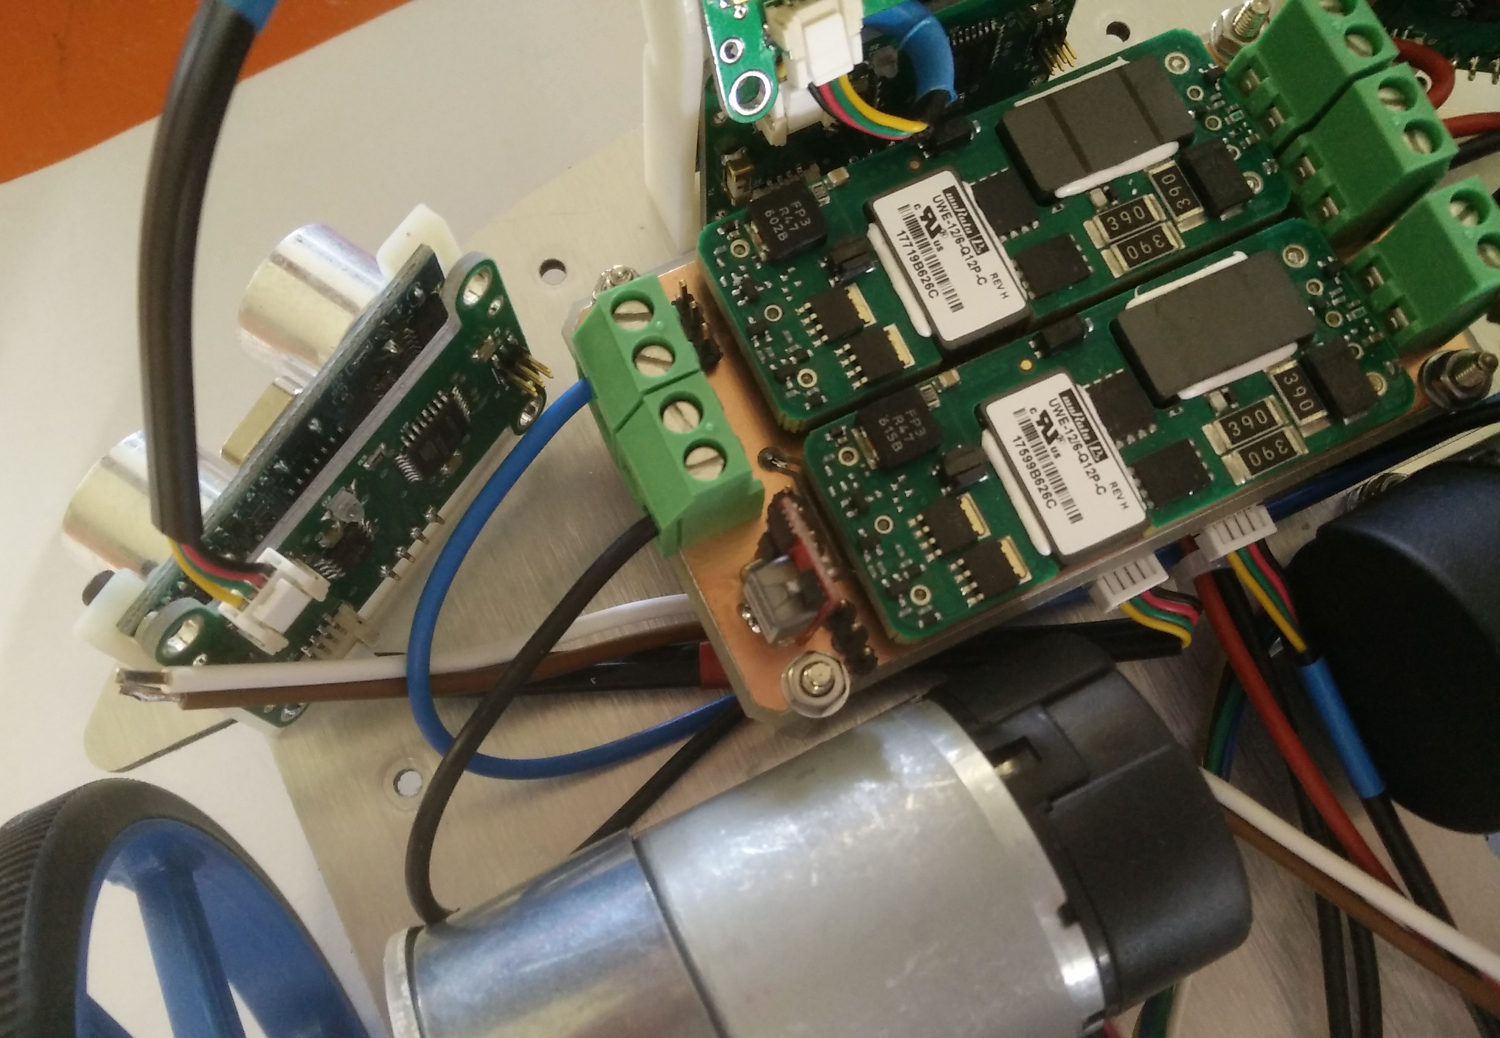
\includegraphics[width=250px]{images/43.jpg}
\caption{Put the wire under the power board.}
\label{fig:43}
\end{figure}

Connect the wire as presented in Figure \ref{fig:44}.

\begin{figure}[H]
\center
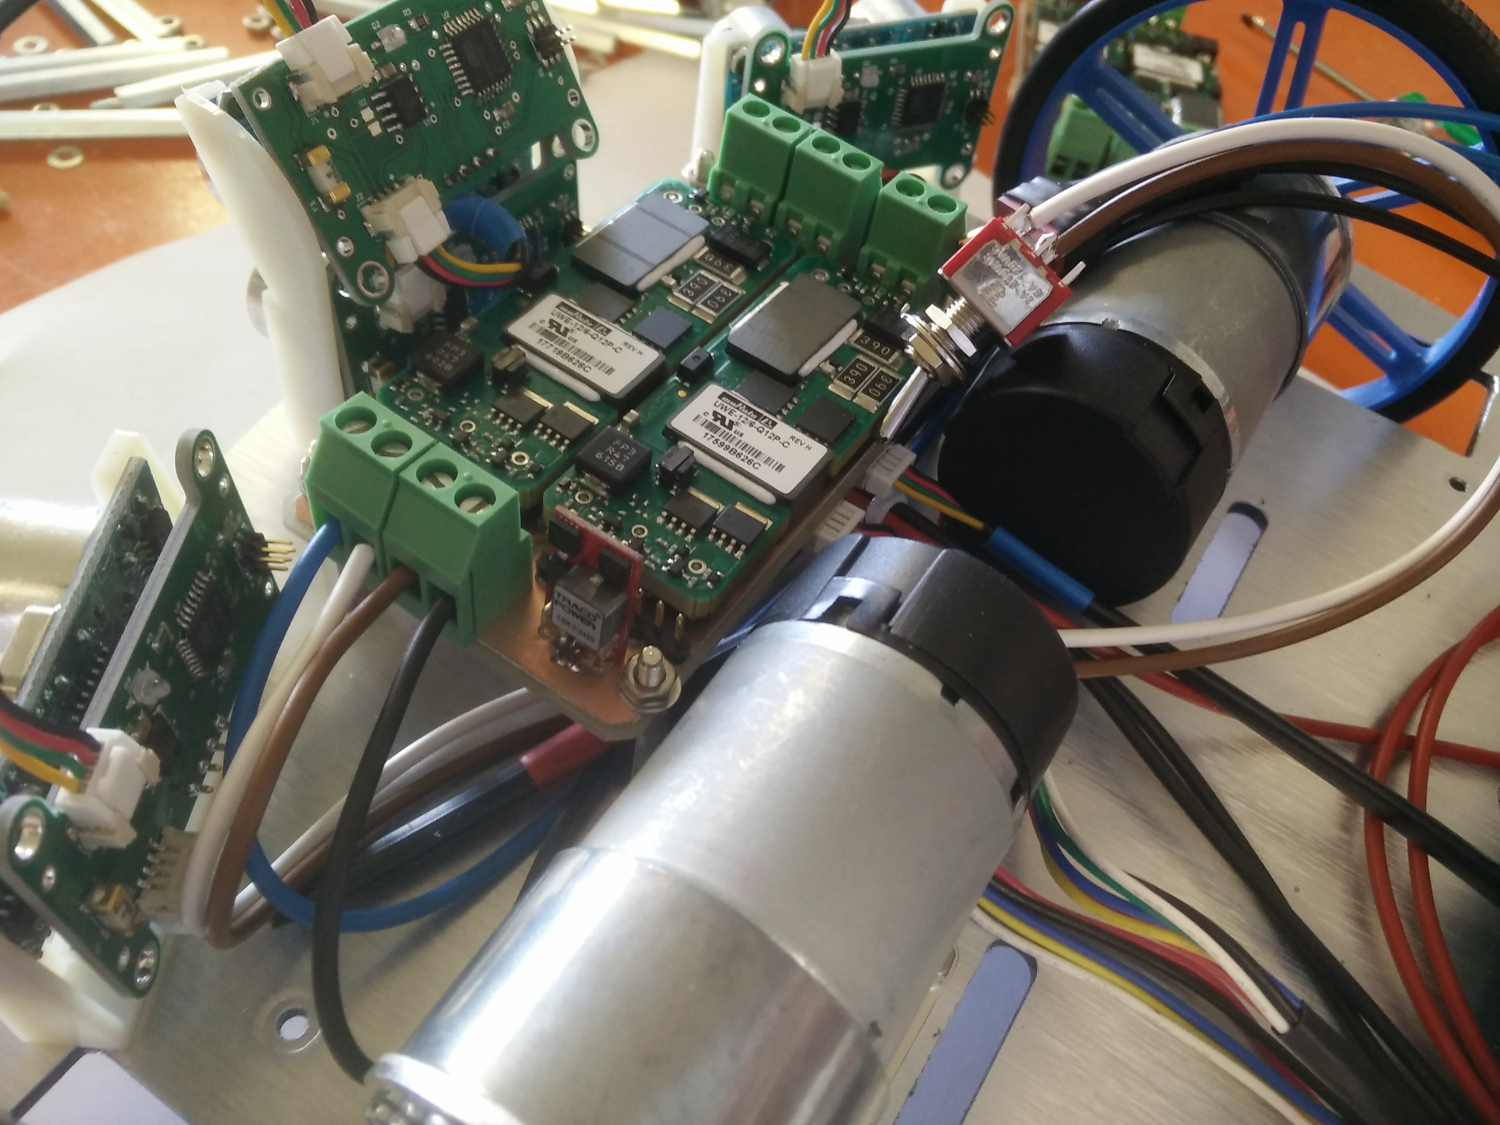
\includegraphics[width=250px]{images/44.jpg}
\caption{Connect the switch.}
\label{fig:44}
\end{figure}

\section{The Batterie}

Now it is possible to set the batterie (Figure \ref{fig:45}) in place. 

\begin{figure}[H]
\center
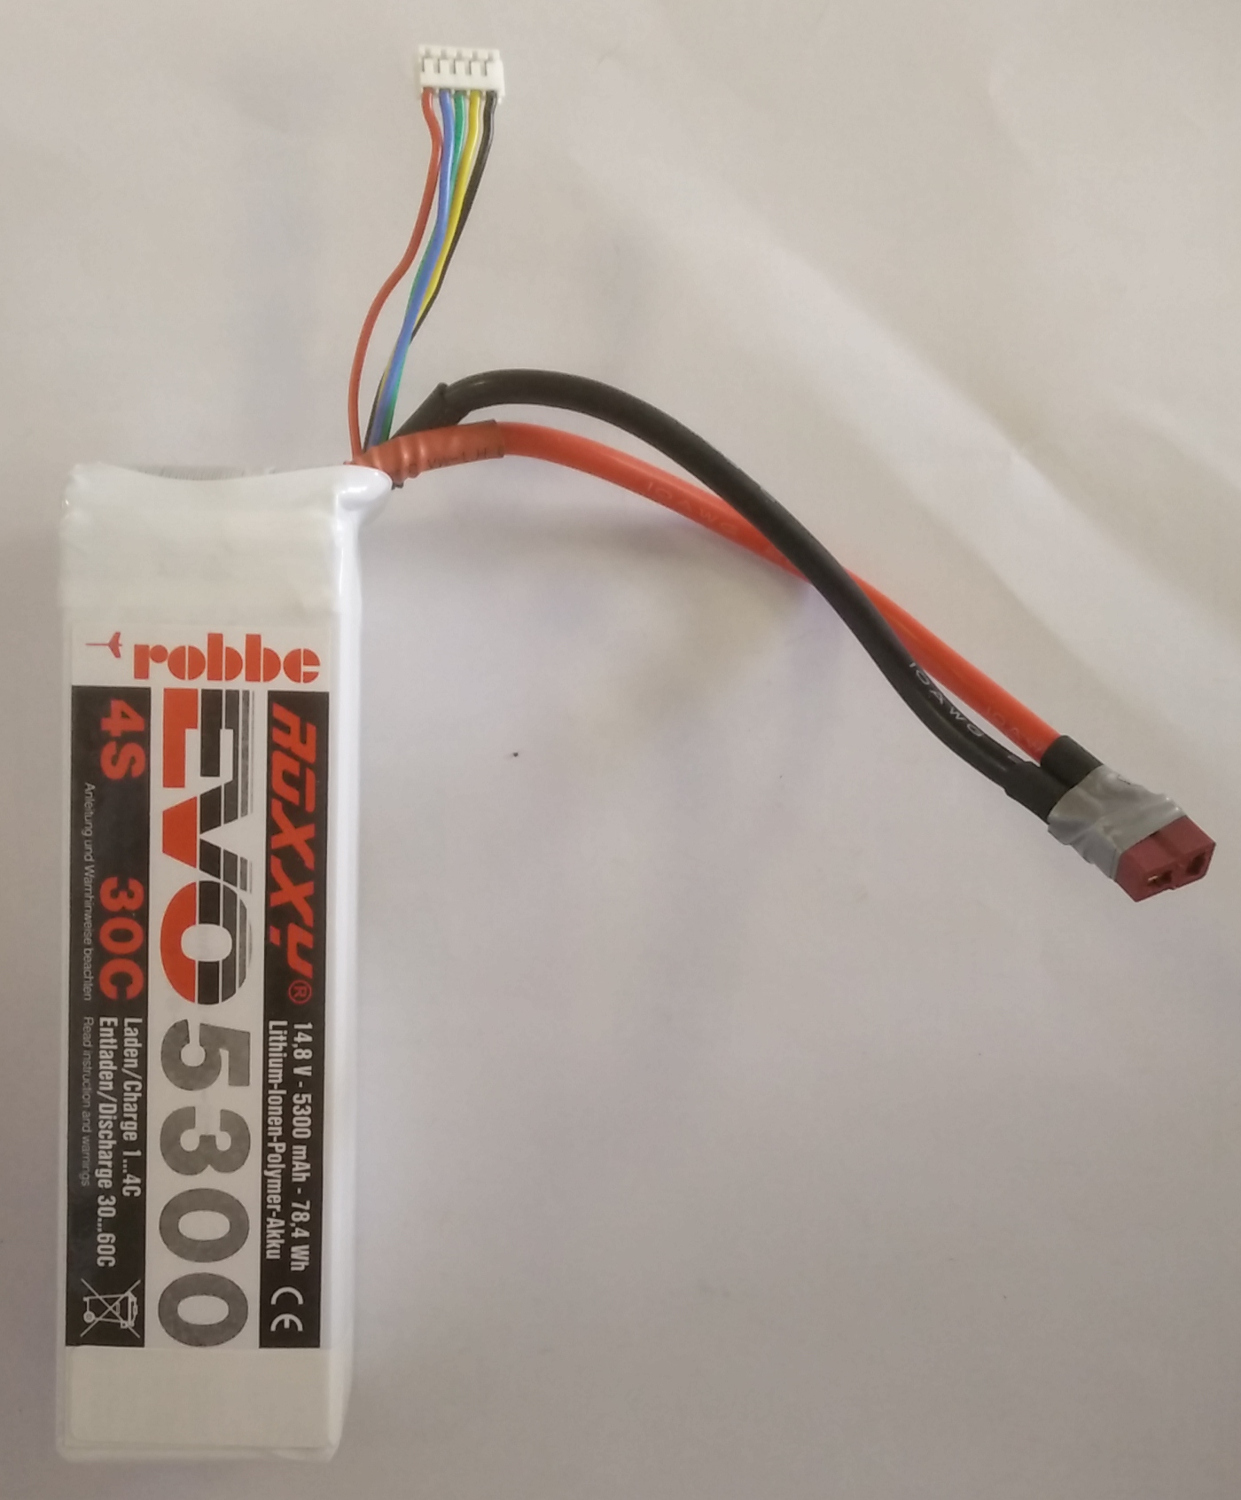
\includegraphics[width=150px]{images/45.jpg}
\caption{The batterie.}
\label{fig:45}
\end{figure}

Place the batterie as depicted in Figure \ref{fig:46}. \textbf{Mind the wire positions!}.

\begin{figure}[H]
\center
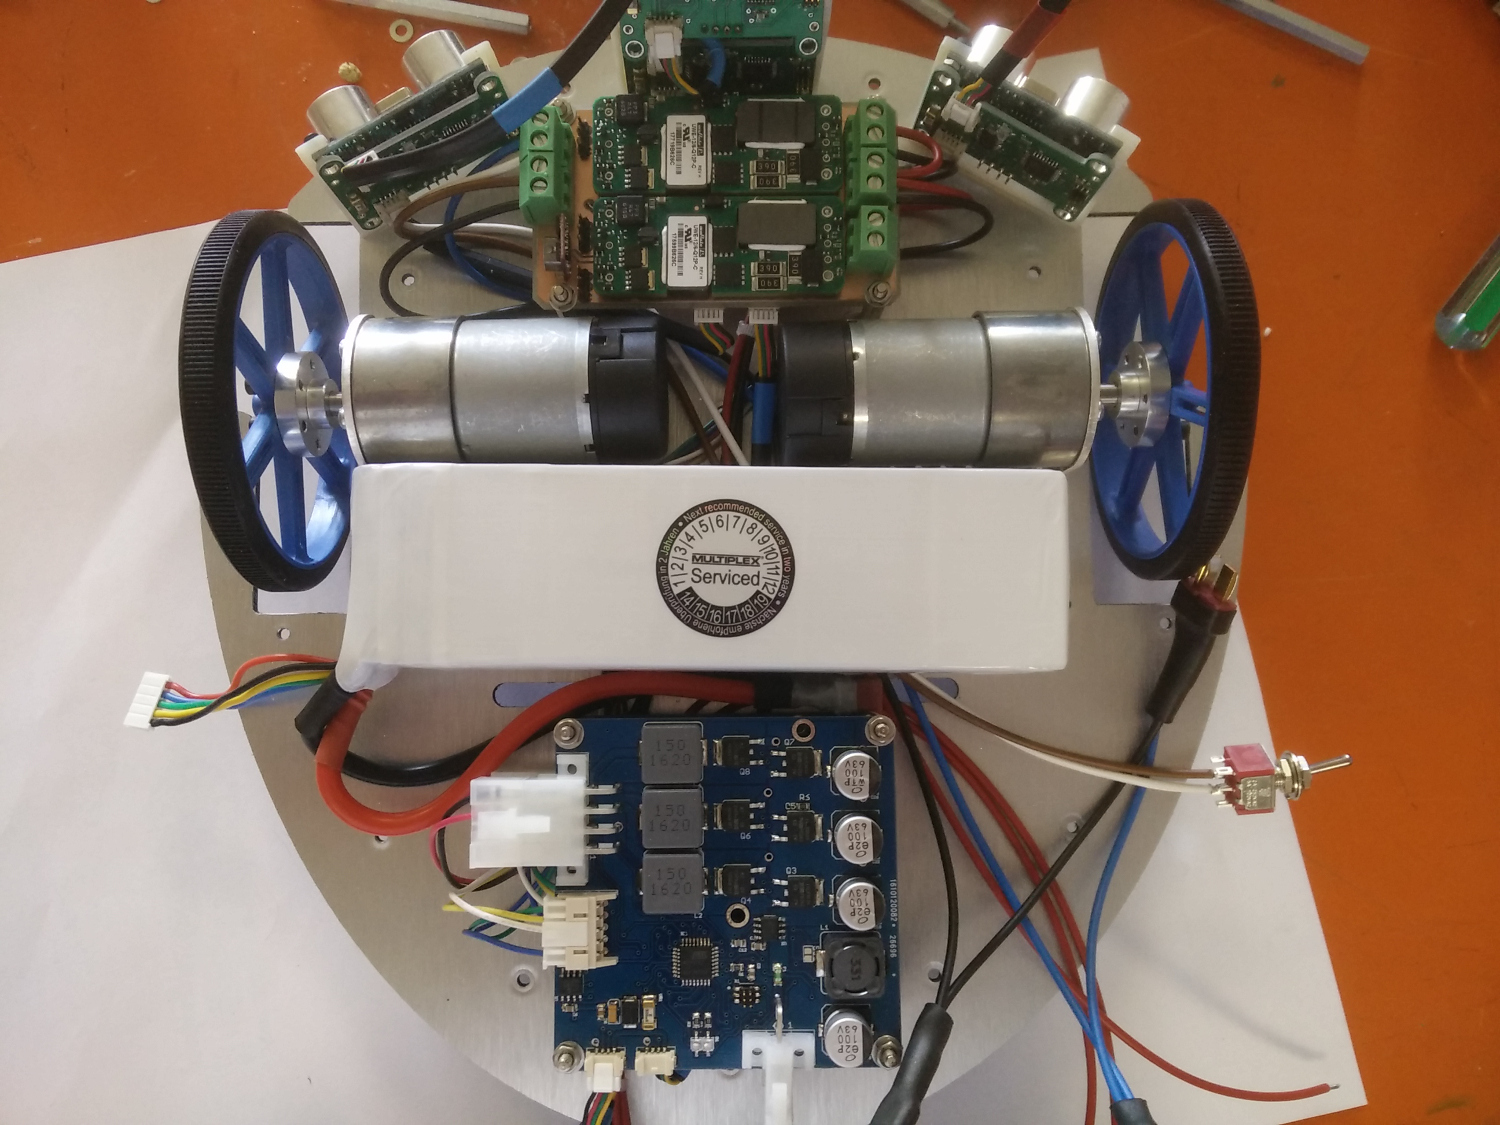
\includegraphics[width=250px]{images/46.jpg}
\caption{The batterie place.}
\label{fig:46}
\end{figure}

 You can use several securing straps to stabilize the batterie as presented in Figure \ref{fig:47}.

\begin{figure}[H]
\center
\includegraphics[width=200px]{images/47.jpg}
\caption{Fixing the batterie.}
\label{fig:47}
\end{figure}

\section{Spacers for the second plate}

The first level is almost done. Now it is needed to place all the 14 spacers depicted in Figure \ref{fig:48}. 

\begin{figure}[H]
\center
\includegraphics[width=200px]{images/48.jpg}
\caption{Spacers for the second plate.}
\label{fig:48}
\end{figure}

You should have the result depicted in Figure \ref{fig:49}.

\begin{figure}[H]
\center
\includegraphics[width=200px]{images/49.jpg}
\caption{Result with the spacers.}
\label{fig:49}
\end{figure}

\section{Last CAN Bus wire before the next level}

Before finishing with the first level, you need to connect a B4 wire (Blue, 20cm) to the motor board as depicted in Figure \ref{fig:49_2}, optaining now the result depicted in Figure \ref{fig:49_3}.

\begin{figure}[H]
\center
\includegraphics[width=200px]{images/49_2.jpg}
\caption{B4 CAN wire to the motor board.}
\label{fig:49_2}

\end{figure}
\begin{figure}[H]
\center
\includegraphics[width=200px]{images/49_3.jpg}
\caption{End of the first plate.}
\label{fig:49_3}
\end{figure}

%%%%%%%%%%%%%%%%%%%%%%%%%%%%%%%%%%%%%%%%%%%%%%%%%%%%%%%%%%%%%%%%%%%%%%%%

\chapter{Second plate}

Now let the first level on the side and take the second plate with the name of the robot (Figure \ref{fig:50}).

\begin{figure}[H]
\center
\includegraphics[width=200px]{images/50.jpg}
\caption{The second plate.}
\label{fig:50}
\end{figure}

\section{Emergency stop button}

Take the bottom of the emergency button (Figure \ref{fig:51}) and fix it on the second plate (Figure \ref{fig:52})

\begin{figure}[H]
\center
\includegraphics[width=350px]{images/51.jpg}
\caption{Emergency button components.}
\label{fig:51}
\end{figure}

\begin{figure}[H]
\center
\includegraphics[width=350px]{images/52.jpg}
\caption{Emergency button bottom fixed.}
\label{fig:52}
\end{figure}

\section{Power loading connectic}

Now you need to fix the power loading connectic. The components are depicted in Figure \ref{fig:53} and the expected results in Figure \ref{fig:54}.

\begin{figure}[H]
\center
\includegraphics[width=100px]{images/53.jpg}
\caption{Batterie loading connectic components.}
\label{fig:53}
\end{figure}

\begin{figure}[H]
\center
\includegraphics[width=250px]{images/54.jpg}
\caption{Batterie loading connectic in place.}
\label{fig:54}
\end{figure}

\section{Spacers for Arduino and Raspberry pi}

Put the spacers Figure \ref{fig:55} in order to obtain the results depicted in Figure \ref{fig:56}.

\begin{figure}[H]
\center
\includegraphics[width=200px]{images/55.jpg}
\caption{Raspberry and Arduino spacers.}
\label{fig:55}
\end{figure}

\begin{figure}[H]
\center
\includegraphics[width=300px]{images/56.jpg}
\caption{Placed Raspberry and Arduino spacers.}
\label{fig:56}
\end{figure}

 Note that in Figure \ref{fig:56} the PiCam is already in place. Once you have screwed the spacers, you can fix the PiCam shown in Figure \ref{fig:57} to fully have the result of Figure \ref{fig:56}.

\begin{figure}[H]
\center
\includegraphics[width=200px]{images/57.jpg}
\caption{PiCam components.}
\label{fig:57}
\end{figure}

\section{Fixing the Arduino and the Raspberry}

Now it is time to place the Arduino and the Raspberry Pi, Figure \ref{fig:58}.
\begin{figure}[H]
\center
\includegraphics[width=150px]{images/58.jpg}
\caption{The Raspberry Pi (left) and the Arduino (right).}
\label{fig:58}
\end{figure}

\subsection{Fixing the Arduino}

Using three nuts, fix the Arduino as depicted in Figure \ref{fig:60}.

\begin{figure}[H]
\center
\includegraphics[width=250px]{images/60.jpg}
\caption{Fixing the Arduino.}
\label{fig:60}
\end{figure}

\subsection{Connecting the PiCam}

Connect the PiCam to the Raspberry as presented in Figure \ref{fig:59}.

\begin{figure}[H]
\center
\includegraphics[width=150px]{images/59.jpg}
\caption{Connecting the PiCam.}
\label{fig:59}
\end{figure}

\subsection{The Arduino and Raspberry CANBus shields}

First, place the spacers Figure \ref{fig:61} as depicted in Figure \ref{fig:62}. 

\begin{figure}[H]
\center
\includegraphics[width=150px]{images/61.jpg}
\caption{Raspberry CAN shield spacers.}
\label{fig:61}
\end{figure}

\begin{figure}[H]
\center
\includegraphics[width=100px]{images/62.jpg}
\caption{Placed Raspberry CAN shield spacers.}
\label{fig:62}
\end{figure}

Then put the Raspberry CAN shield (blue) and the Arduino CAN shield (yellow) as depicted in Figure \ref{fig:63}.

\begin{figure}[H]
\center
\includegraphics[width=300px]{images/63.jpg}
\caption{Placing the CAN shields.}
\label{fig:63}
\end{figure}

 Use nuts to well fix the Raspberry CAN shield, as presented in Figure \ref{fig:64}.

\begin{figure}[H]
\center
\includegraphics[width=200px]{images/64.jpg}
\caption{Nuts for the Raspberry CAN shield.}
\label{fig:64}
\end{figure}

\subsection{Spacers for the last plate}

Before assembling the first and the second plate, it is needed to screw the spacers for the last plate. Assemble the spacers as depicted in Figure \ref{fig:65_2} and fix them on the second plate as depicted in Figure \ref{fig:65_3}.

\begin{figure}[H]
\center
\includegraphics[width=200px]{images/65_2.jpg}
\caption{Spacers for the last plate.}
\label{fig:65_2}
\end{figure}

\begin{figure}[H]
\center
\includegraphics[width=350px]{images/65_3.jpg}
\caption{Spacers for the last plate in place.}
\label{fig:65_3}
\end{figure}


%%%%%%%%%%%%%%%%%%%%%%%%%%%%%%%%%%%%%%%%%%%%%%%%%%%%%%%%%%%%%%%%%%%%%%%%
\chapter{Assembling the first and the second plate}

Now that the second plate is done, it is possible to unify what have been done so far.

\section{The batterie}
First, connect the batterie connectors of Figure \ref{fig:65} as shown in Figure \ref{fig:66} while putting the second plate on the first one. 

\begin{figure}[H]
\center
\includegraphics[width=200px]{images/65.jpg}
\caption{The batterie connectors.}
\label{fig:65}
\end{figure}

\begin{figure}[H]
\center
\includegraphics[width=200px]{images/66.jpg}
\caption{Connection of the batterie connectors.}
\label{fig:66}
\end{figure}

\textbf{Warning: While placing the second plate on the first one, be carefull with the wires!} Put them as depicted in Figure \ref{fig:67}.

\begin{figure}[H]
\center
\includegraphics[width=400px]{images/67.jpg}
\caption{Mind the wires!}
\label{fig:67}
\end{figure}

\section{The ON/OFF button}

Before fixing the second plate on the first one, you need to put the ON/OFF switch, as depicted in Figure \ref{fig:68}. \textbf{Do it clean, the switch must be just above the plate!}

\begin{figure}[H]
\center
\includegraphics[width=300px]{images/68.jpg}
\caption{The ON/OFF switch in place.}
\label{fig:68}
\end{figure}

\section{Wiring the CAN Bus for the Arduino and the Raspberry}

Connect the Raspberry CAN bus shield and the Arduino CAN bus shield with the CAN bus wires that go from the first level to the second one, as depicted in Figure \ref{fig:69}.

\begin{figure}[H]
\center
\includegraphics[width=300px]{images/69.jpg}
\caption{Connection of the Raspberry and the Arduino to the CAN bus.}
\label{fig:69}
\end{figure}

\section{Wiring the emergency stop button}

From the three wires that arise from the emergency stop bottom, identify the two wires that are connected to the motor boards (continuity test) as depicted in Figure \ref{fig:70}.

\begin{figure}[H]
\center
\includegraphics[width=300px]{images/70.jpg}
\caption{Identifying the two motor board connected wires.}
\label{fig:70}
\end{figure}

Wire those two wires to the emmergency stop button connector, and finally wire the remaining red wire to the other side of the connector as depicted in Figure \ref{fig:71}.

\begin{figure}[H]
\center
\includegraphics[width=150px]{images/71.jpg}
\caption{Connection of the wires to the emmergency stop connector.}
\label{fig:71}
\end{figure}

\section{Fixing the second plate}

Finally, using the screws depicted in Figure \ref{fig:72}, fix the second plate to the corresponding spacers in order to have the result presented in Figure \ref{fig:73}.

\begin{figure}[H]
\center
\includegraphics[width=150px]{images/72.jpg}
\caption{The screws to fix the second plate.}
\label{fig:72}
\end{figure}


\begin{figure}[H]
\center
\includegraphics[width=200px]{images/73.jpg}
\caption{The second plate assembled.}
\label{fig:73}
\end{figure}

The last thing to do for the second plate: adding the top of the emergency stop button and obtain the result depicted in Figure \ref{fig:74}.

\begin{figure}[H]
\center
\includegraphics[width=150px]{images/74.jpg}
\caption{Adding the emergency stop button top.}
\label{fig:74}
\end{figure}


%%%%%%%%%%%%%%%%%%%%%%%%%%%%%%%%%%%%%%%%%%%%%%%%%%%%%%%%%%%%%%%%%%%%%%%%

\chapter{Third and last plate}

Now it is time to assemble the third and last plate: the top of the robot. The plate is shown in Figure \ref{fig:75}.

\begin{figure}[H]
\center
\includegraphics[width=150px]{images/75.jpg}
\caption{Top plate.}
\label{fig:75}
\end{figure}

\section{The Human Machine Interface buttons}

The needed components to fix the buttons are depicted in Figure \ref{fig:76}.

\begin{figure}[H]
\center
\includegraphics[width=150px]{images/76.jpg}
\caption{The button components.}
\label{fig:76}
\end{figure}

Fix the buttons to have the results presented in Figure \ref{fig:77}. \textbf{Warning : be shure that the buttons can be pressed and are well released, we do not want the plate to bother the buttons!}

\begin{figure}[H]
\center
\includegraphics[width=350px]{images/77.jpg}
\caption{The fixed buttons.}
\label{fig:77}
\end{figure}

\section{The Human Machine Interface LCD screen}

The next step is fixing the screen to the plate. The needed components are depicted in Figure \ref{fig:78}.

\begin{figure}[H]
\center
\includegraphics[width=150px]{images/78.jpg}
\caption{The screen components.}
\label{fig:78}
\end{figure}

Fix the screen to obtain the result presented in Figure \ref{fig:79}

\begin{figure}[H]
\center
\includegraphics[width=150px]{images/79.jpg}
\caption{The fixed screen.}
\label{fig:79}
\end{figure}

\section{The IMU support}

Fix the spacers depicted in Figure \ref{fig:80} in order to have the result presented in Figure \ref{fig:81}.

\begin{figure}[H]
\center
\includegraphics[width=100px]{images/80.jpg}
\caption{The IMU spacers.}
\label{fig:80}
\end{figure}

\begin{figure}[H]
\center
\includegraphics[width=300px]{images/81.jpg}
\caption{The fixed IMU spacers.}
\label{fig:81}
\end{figure}

Then fix the IMU support as presented in Figure \ref{fig:82}.

\begin{figure}[H]
\center
\includegraphics[width=300px]{images/82.jpg}
\caption{The fixed IMU support.}
\label{fig:82}
\end{figure}

\section{The LiDAR}

Now fix the LiDAR depicted in Figure \ref{fig:83} to have the result depicted in Figure \ref{fig:84}.

\begin{figure}[H]
\center
\includegraphics[width=200px]{images/83.jpg}
\caption{The LiDAR.}
\label{fig:83}
\end{figure}

\begin{figure}[H]
\center
\includegraphics[width=300px]{images/84.jpg}
\caption{The fixed LiDAR.}
\label{fig:84}
\end{figure}

\section{Fixing the third plate}

Almost done, the last plate can be fixed to the robot, as presented in Figure \ref{fig:85}.

\begin{figure}[H]
\center
\includegraphics[width=300px]{images/85.jpg}
\caption{Fixing the last plate.}
\label{fig:85}
\end{figure}

\section{Connecting the screen to the CAN Bus}

The last step is to link the highest level to the other ones using the CAN Bus. To do so, connect a B6 wire (Blue, 16cm) to the screen and the Raspberry as depicted in Figure \ref{fig:86}.


\begin{figure}[H]
\center
\includegraphics[width=300px]{images/86.jpg}
\caption{Connecting the screen to the CAN Bus.}
\label{fig:86}
\end{figure}

%%%%%%%%%%%%%%%%%%%%%%%%%%%%%%%%%%%%%%%%%%%%%%%%%%%%%%%%%%%%%%%%%%%%%%%%

\chapter{Result}

You should now have a fully assembled IstiaBot, as presented in Figure \ref{fig:87}.

\begin{figure}[H]
\center
\includegraphics[width=350px]{images/87.jpg}
\caption{IstiaBot.}
\label{fig:87}
\end{figure}




\end{document}
